\chapter{Gamma detection in medicine}\label{chap::2}

\vfill

\minitoc

\newpage

\glsresetall

As described in chapter~\ref{chap::1}, the detection of gamma photons plays a role of utmost importance in medical physics, for what concerns both the monitoring of ion beam therapy treatments and the nuclear medicine examination techniques. 

Ion beam therapy is rapidly emerging as a valuable cancer treatment technique and a superior alternative to photon radiotherapy for specific clinical indications. The narrow dose peak at the end of the ion range allows for targeted delivery of high dose to the tumor while sparing healthy surrounding tissues. However, since such a treatment technique is highly sensitive to dose prediction and delivery uncertainties, online range monitoring solutions are necessary. Over- and under-shooting effects potentially lead to severe damages to healthy tissues and/or treatment inefficiency, and thus have to be controlled in real-time. The research effort in this field mainly focuses on the non-invasive detection of primary by-products of beam-tissue nuclear interactions: photons from electron-positron annihilation and prompt gammas are most extensively studied for this purpose. 

In nuclear medicine diagnostics, radioactive tracers are injected in the patient body and the gamma rays, products of the tracer isotope decay, exiting the patient are detected to retrieve physiological and anatomical information. Positrons are emitted by $\beta^+$-decaying isotopes, and the two back-to-back photons generated by their annihilation with patient electrons are detected in time coincidences in \gls{pet} techniques. On the other hand, \gls{spect} exploits single photons emitted by $\gamma$-decaying isotopes with collimated detectors.

The research work presented in this thesis focus on the development of gamma cameras for the detection of prompt gamma rays to tackle the challenge of real-time range monitoring during particle therapy treatments. In addition, the developed prototype design has been tested for application in nuclear medicine \gls{spect}-like examinations. 
In this chapter, after a brief introduction about the photon interaction channels in matter, the main techniques based on gamma detection developed in the two mentioned fields are described, and the state-of-the-art of gamma detectors employed for these two purposes is sketched.

\section{Photon interactions in matter}\label{chap2::subsec::PhotonInteractions}

In penetrating an absorbing medium, photons may experience various interactions with the atoms of the medium, involving either the nuclei or the orbital electrons. The interactions with nuclei may be direct photon-nucleus collisions or interactions between the photon and the electrostatic field of the nucleus (pair production). On the other hand, the photon-orbital electron interactions can involve either loosely bound electrons (binding energy $E_B$ small in comparison with the photon energy $h\nu$ - $E_B \ll h\nu$) or tightly bound electrons (binding energy comparable to, or slightly smaller than the photon energy - $E_B  \lesssim h\nu$). 
All these processes are characterized by a partial or complete energy transfer of the gamma-ray photon, and two different outcomes are possible:
\begin{itemize}
\item Photon disappears (i.e. is completely absorbed) and its energy is transferred to light charged particles (electron and positrons);
\item Photon is scattered and two results are possible:
	\begin{itemize}
		\item the resulting photon has the same energy as the incident photon and no light charged particle is released in the interaction;
		\item the resulting scattered photon has a lower energy than the incident photon and the energy excess is transferred to a light charged particle (electron).
	\end{itemize}
\end{itemize}

We focus here on the interaction channels which play an important role in radiation measurements: 
\begin{itemize}
\item photoelectric absorption;
\item Compton scattering;
\item pair production.
\end{itemize}

In case the photon interacts with an absorber \myMarginnote{Photoelectric absorption} atom and completely disappears by transferring all its energy to the target, the interaction mechanism is called photoelectric absorption. In the interaction an orbital electron  is ejected with kinetic energy $E_K$ corresponding to the difference between the incident photon energy $h\nu$ and the electron binding energy $E_B$, as reported in equation~\ref{chap2::eq::energyPhotoelectron}. The ejected orbital electron is generally referred to as \enquote{photoelectron}. A schematic view of the photoelectric absorption mechanism is shown in \figurename~\ref{chap2::fig::photoel_abs}.

\begin{equation}
E_K = h\nu - E_B
\label{chap2::eq::energyPhotoelectron}
\end{equation}

\begin{figure}[!htbp]
\centering
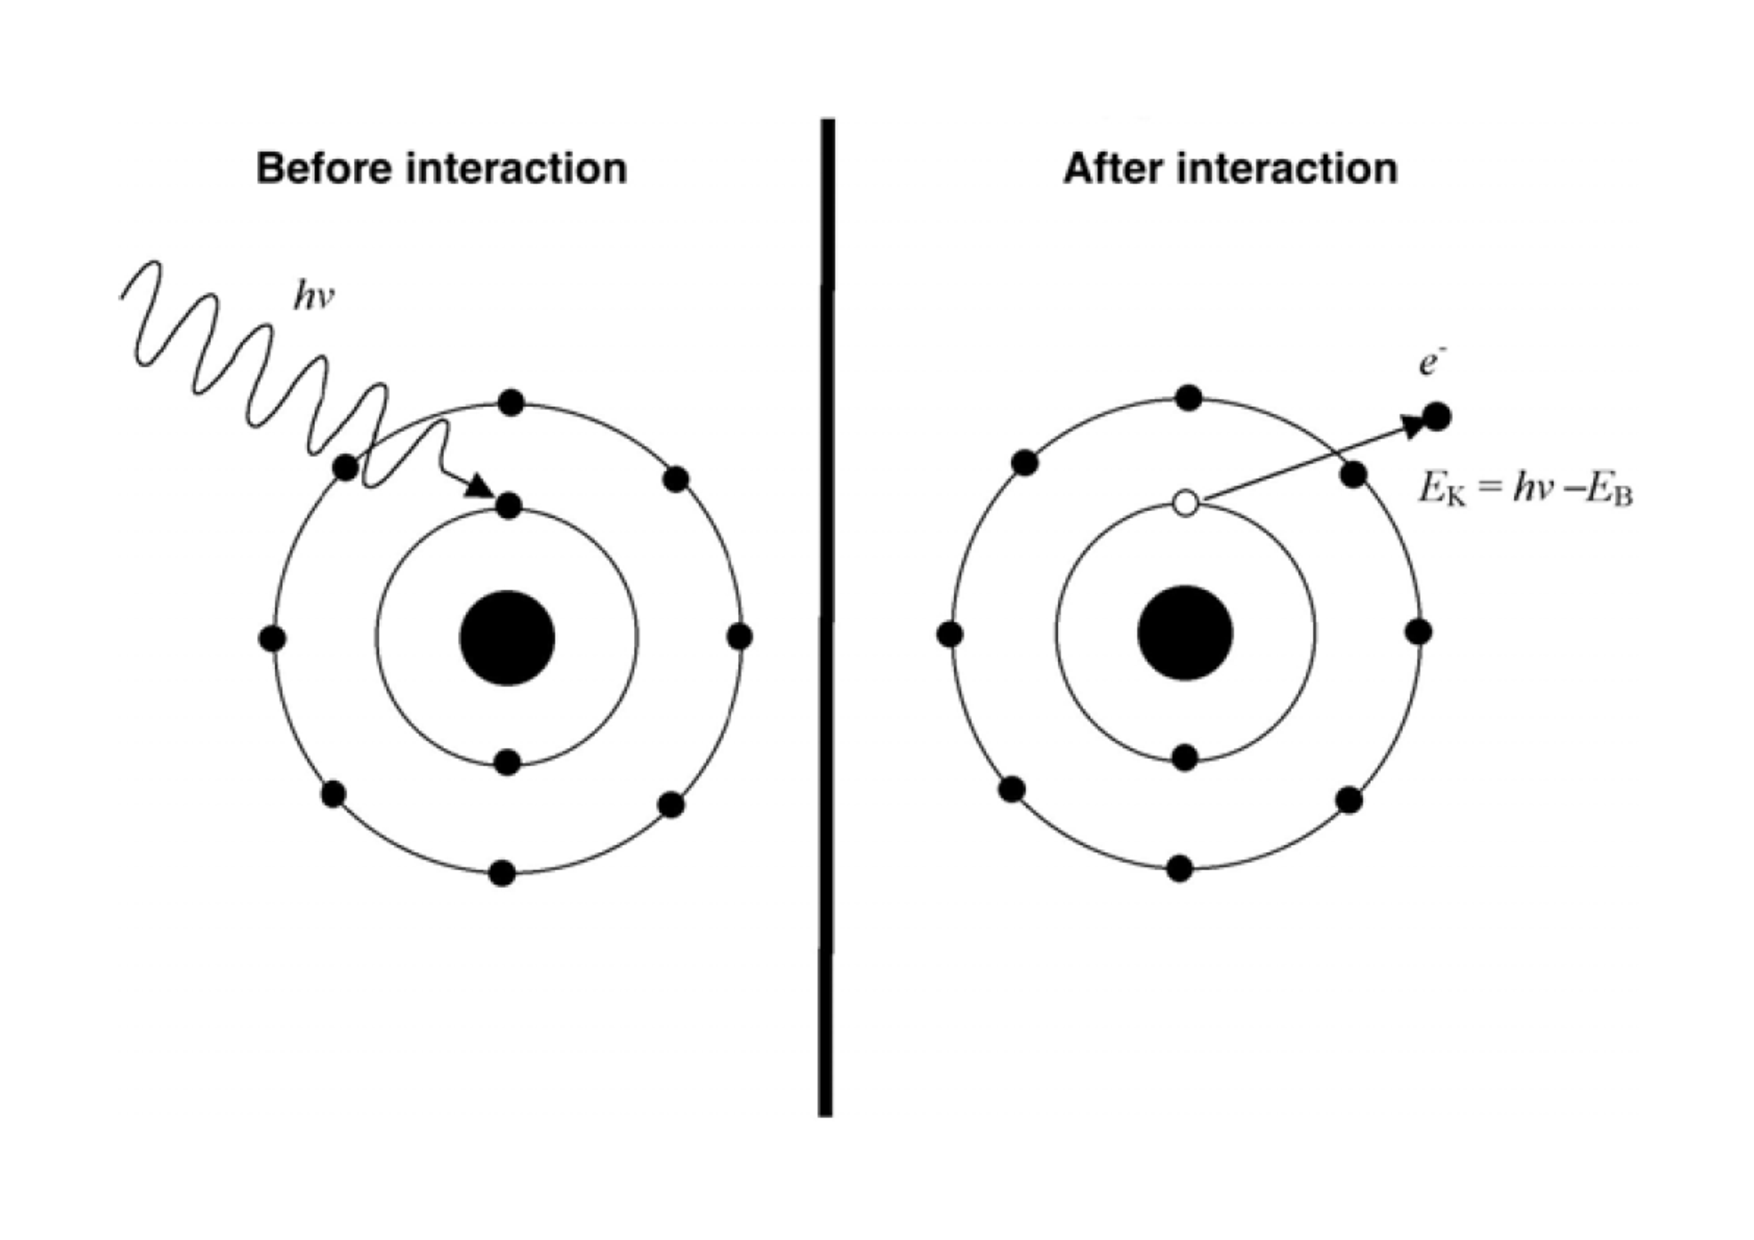
\includegraphics[width=0.8\textwidth]{03_GraphicFiles/chapter2_GammaCameras/photoelectric_abs.pdf}
\caption{Schematic diagram of the photoelectric effect. A photon with energy $h \nu$ interacts with a K-shell electron, which is ejected as photoelectron with kinetic energy $E_K$. In~\cite{Podgorsak2010}.}
\label{chap2::fig::photoel_abs}
\end{figure} 

The interaction is with the atom as a whole, and cannot take place with free electrons for conservation of energy and momentum constraints, although the whole photon energy is transferred to an atomic electron in one of the atom bound shells (tightly bound electron). Energy and momentum cannot be conserved simultaneously in a photon-free electron interaction: the momentum conservation requires a third object (the atom) involved in the interaction which must absorb the extra momentum. When the photon energy exceeds the K-shell binding energy of the absorber, about 80\% of all photoelectric absorption interactions occur with the K-shell electrons. If the energy transferred to the photoelectron is not below the binding energy threshold, it can be sufficient to raise it to a higher orbit, in a process of excitation. 
As a result of the photoelectric absorption, in addition to the ejected photoelectron, the absorber atom has a vacancy in one of its bound shells. This vacancy is quickly filled through capture of a free electron of the medium and/or rearrangement of electrons from other shells at higher energy level. Therefore, depending on the involved shells, one or more characteristics x-ray photons (fluorescent photons) may also be generated. Such photons are generally reabsorbed close to the original atom site through a further photoelectric absorption involving less tightly bound shells. In some fraction of the cases, the emission of an Auger electron may substitute for the characteristic x-ray in carrying away the atomic excitation energy. As the fluorescent photons, Auger electrons are generally reabsorbed very near the site of the original interaction.
The photoelectric process is the predominant mode of interaction for gamma rays of relatively low energy, and it is also enhanced for absorber materials of high atomic number Z. Even if a single analytic expression for the probability of photoelectric absorption over all ranges of photon energy $E_{\gamma}$ and Z, the probability ($\sigma_{PE}$)dependence on these two parameters can be approximated as shown in equation~\ref{chap2::eq::photoelProb}, where $n$ varies in the range [4,5] depending on the photon energy (4 for relatively low photon energies, 5 in the relativistic region)~\parencite{Knoll2000}.

\begin{equation}
\sigma_{PE} \varpropto \frac{Z^n}{E^{3.5}_{\gamma}} 
\label{chap2::eq::photoelProb}
\end{equation}  
 
In \figurename~\ref{chap2::fig::photonCrossSec} the cross section for the photoelectric absorption is compared to the one of the other photon interaction mechanisms for a copper absorber as a function of the photon energy. It exhibits a characteristic sawtooth structure in which the sharp discontinuities arise whenever the photon energy coincides with the binding energy of a particular electron shell. Except for the K shell, all other shells have a fine energy structure which reflect in the cross section curve.  

An interaction of a photon of energy $h\nu$ \myMarginnote{Compton scattering} with a loosely bound orbital electron of an absorber is called Compton scattering in honor of Arthur Compton who made the first measurements of photon-\enquote{free electron} scattering in 1923~\parencite{Compton1923}. Compton earned the Nobel prize for the discovery in 1927.  
In Compton scattering, the incoming gamma-ray photon is deflected through an angle $\theta$ with respect to its original direction, while transferring a portion of its energy to the electron, referred to as \enquote{recoil electron}. In theoretical studies of such an interaction mechanism, an assumption is made that the photon interacts with a free and stationary electron. As a result of the interaction, the photon, which had an initial energy $h\nu$, continue traveling in the new direction (angle $\theta$ with respect to the incident direction) with reduced energy $h\nu'$, and the recoil electron is ejected from the atom with a kinetic energy $E_K$ and a direction with an angle $\phi$ with respect the photon incident direction. A schematic view of the interaction is given in \figurename~\ref{chap2::fig::compton_principle}.
The expression that relates the energy transfer and the scattering angle for any given interaction can be derived by writing simultaneous equations for the conservation of energy and momentum. The obtained relationship is presented in equation~\ref{chap2::eq::Compton}, with the notation described above and $m_{0}c^2$ the rest-mass energy of the electron (511~keV). From the same calculation the kinetic energy of the recoil electron is also obtained from the expression in equation~\ref{chap2::eq::ComptonRecEnergy}.

\begin{equation}
h\nu' = \frac{h\nu}{1+\frac{h\nu}{m_{0}c^2}(1-\cos(\theta))}
\label{chap2::eq::Compton}
\end{equation} 

\begin{equation}
E_K = h\nu \frac{\frac{h\nu}{m_0c^2} (1-\cos(\theta))}{1+\frac{h\nu}{m_{0}c^2}(1-\cos(\theta))}
\label{chap2::eq::ComptonRecEnergy}
\end{equation} 

\begin{figure}[!htbp]
\centering
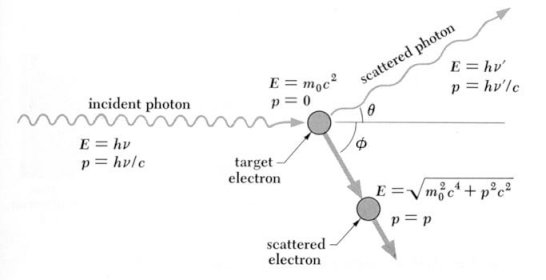
\includegraphics[width=0.8\textwidth]{03_GraphicFiles/chapter2_GammaCameras/ComptonPrinciple.jpg}
\caption{Schematic view of the Compton scattering principle. Image from https://universe-review.ca/R15-12-QFT10.htm.}
\label{chap2::fig::compton_principle}
\end{figure} 

From equation~\ref{chap2::eq::Compton} emerges how small scattering angles correspond to little energy transfers, and the other way around. In particular, for $\theta = 0$, no energy is transferred to the electron and the interaction becomes a classical Thomson scattering. For for $\theta > 0$ the energy of the scattered photon saturates at high values of the incident photon energy; the larger is the scattering angle, the lower is the saturation value of $h\nu'$ for $h\nu \lim \infty$
The relationship between the photon energy before and after the interaction is shown in \figurename~\ref{chap2::fig::ComptonEnergy} for various scattering angles $\theta$ between 0\textdegree (forward scattering) and $\pi$ (back-scattering.) 
The scattering angle $\theta$ and the recoil electron angle $\phi$ are related by equation~\ref{chap2::eq::ComptonAngles}.

\begin{equation}
\cot(\phi) = (1+\frac{h\nu}{m_{0}c^2})\tan\bigg(\frac{\theta}{2}\bigg)
\label{chap2::eq::ComptonAngles}
\end{equation} 

This relationship shows that for a given $\theta$, the higher is the incident photon energy $h\nu$, the smaller is the recoil electron angle $\phi$. In \figurename~\ref{chap2::fig::thetaphirel} the scattering and recoil angle dependence is plotted for different values of $\epsilon = h\nu / m_{0}c^2$.

\begin{figure}
\centering
\begin{subfigure}[t]{.49\textwidth}
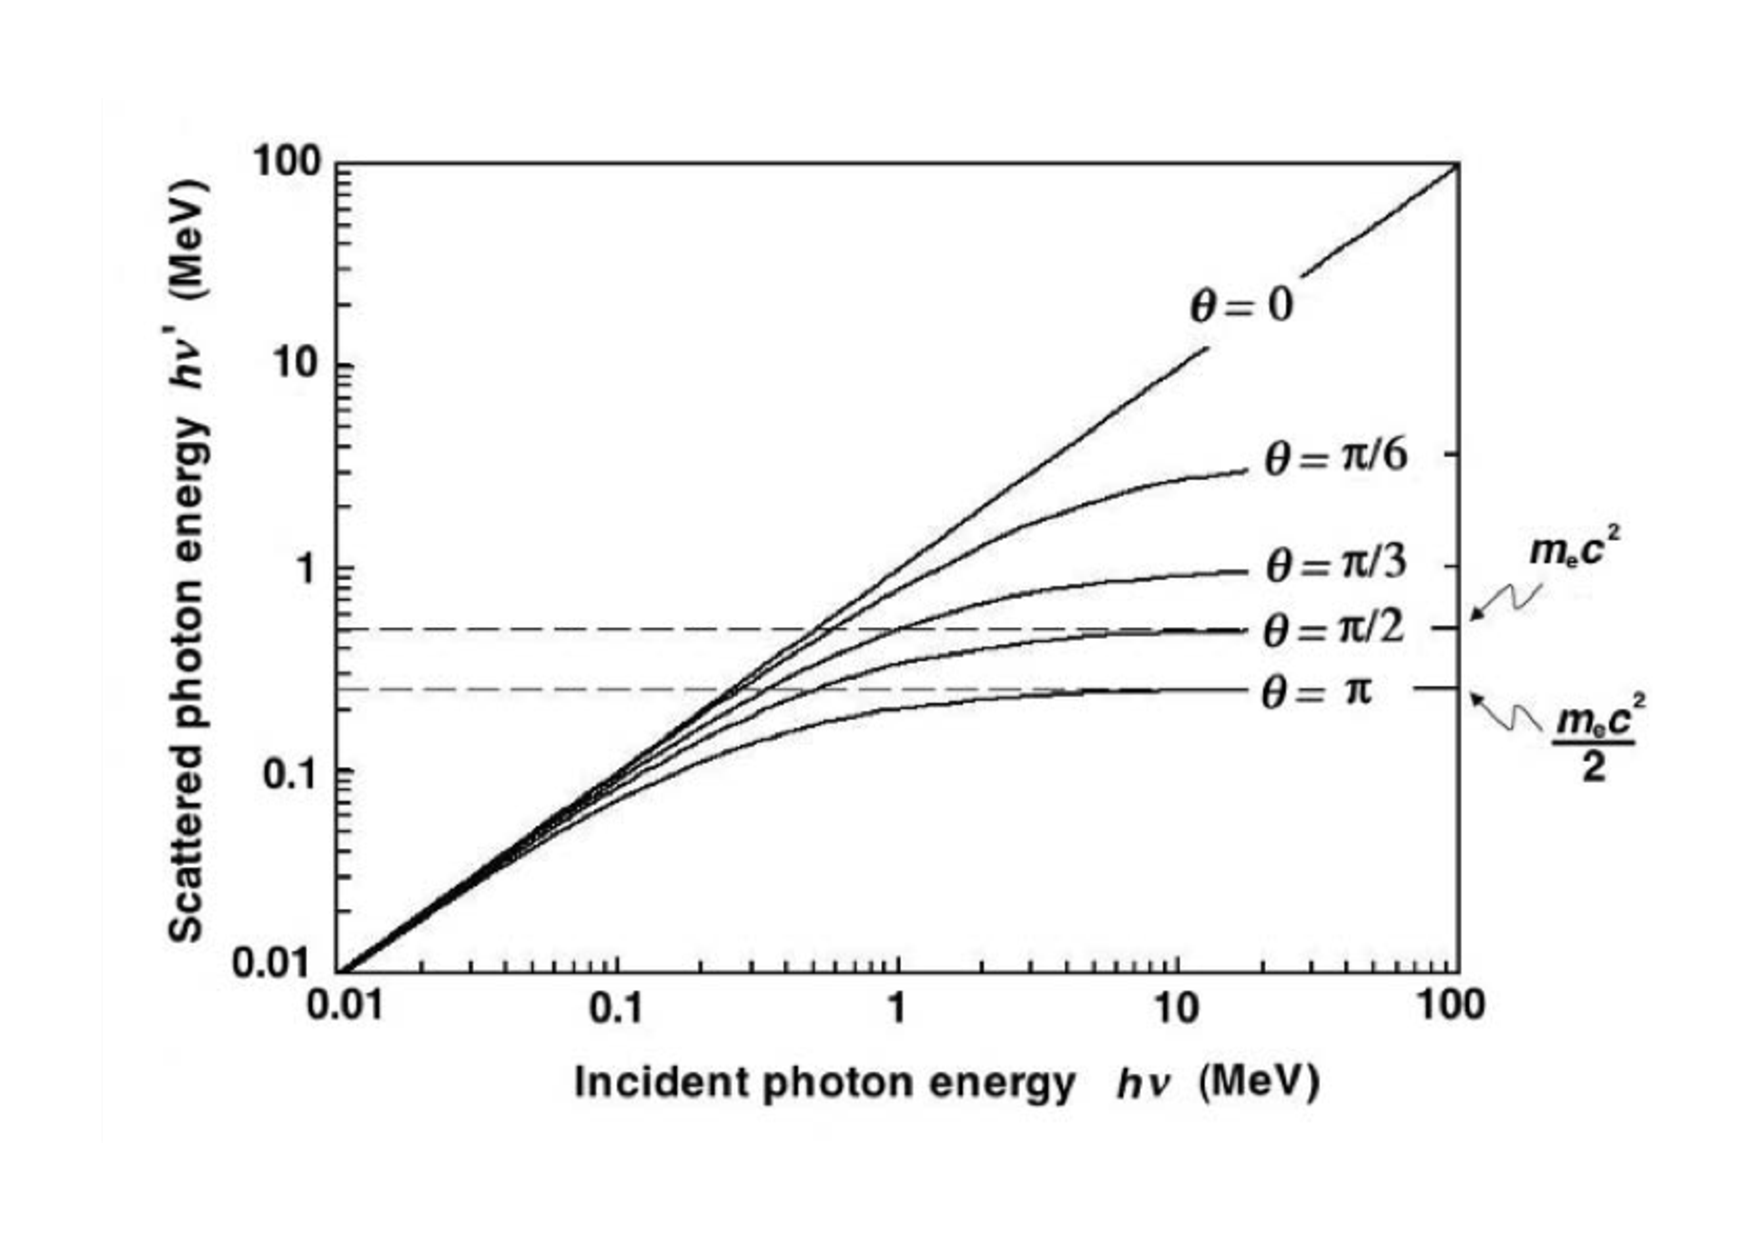
\includegraphics[width=1.1\linewidth]{03_GraphicFiles/chapter2_GammaCameras/ComptonEnergy.pdf}
\caption{Scattered photon energy against the incident photon energy for various Compton scattering angles in the range from 0\textdegree to $\pi$.}
\label{chap2::fig::ComptonEnergy}
\end{subfigure}
\begin{subfigure}[t]{.49\textwidth}
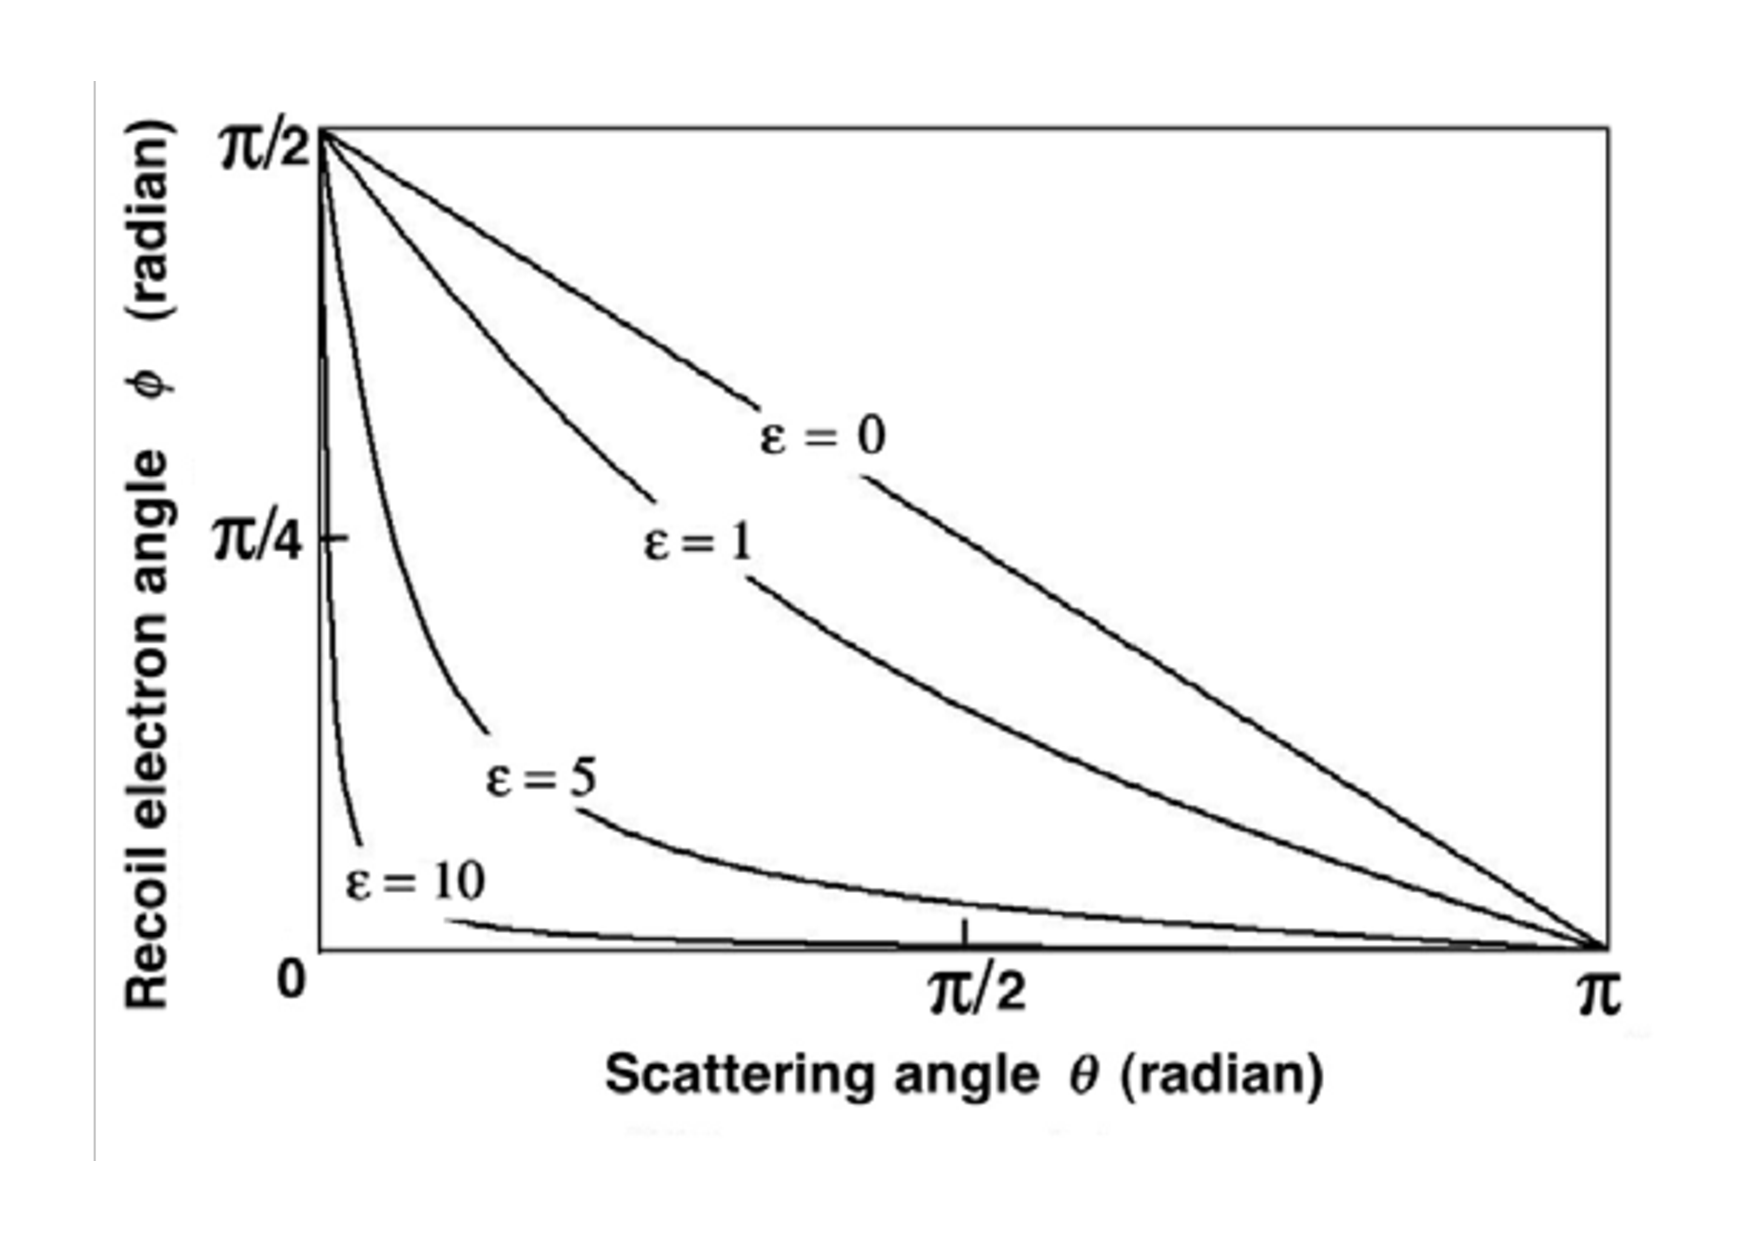
\includegraphics[width=1.1\linewidth]{03_GraphicFiles/chapter2_GammaCameras/scattRecoilAnglesCompton.pdf}
\caption{Relationship between the electron recoil electron $\phi$ and the photon Compton scattering angle $\theta$.}
\label{chap2::fig::thetaphirel}
\end{subfigure}
\caption{In~\cite{Podgorsak2010}}
\label{chap2::fig::ComptonAngular}
\end{figure}
   
The probability of Compton scattering per atom of the absorber depends on the number of electrons available as scattering targets and therefore linearly increases with the atomic number Z. In \figurename~\ref{chap2::fig::photonCrossSec} the probability energy dependence is shown for a copper target and compared to the other interaction channels probability. The differential cross section, or angular distribution of scattered gamma rays, is predicted by a formula derived by Oskar Klein and Yoshio Nishina in 1929, and reported in equation~\ref{chap2::eq::KleinNishina}~\parencite{Klein1929}.
 \begin{equation}
\frac{\mathrm{d}\sigma}{\mathrm{d}\Omega} = Zr_{e}\bigg(\frac{1}{1+\epsilon (1-\cos(\theta))}\bigg)^{2}\bigg( \frac{1+\cos^2(\theta)}{2} \bigg)\bigg(1+\frac{\epsilon^2(1-\cos(\theta))^2}{(1+\cos^2(\theta)[1+\epsilon(1-\cos(\theta))])} \bigg) 
\label{chap2::eq::KleinNishina}
\end{equation} 
where $r_{e}$ is the classical electron radius expressed in equation~\ref{chap1::eq::electronRad}. The distribution is shown graphically in \figurename~\ref{chap2::fig::ComptonAngCrossSection} and illustrates the strong tendency for forward scattering at high values of the gamma-ray energy. At low incident photon energies the probability for forward scattering and back-scattering are equal and twice as large as the probability for side scattering. As the incident photon energy increases, the scattering becomes increasingly more forward peaked and back-scattering rapidly diminishes.

\begin{figure}[!htbp]
\centering
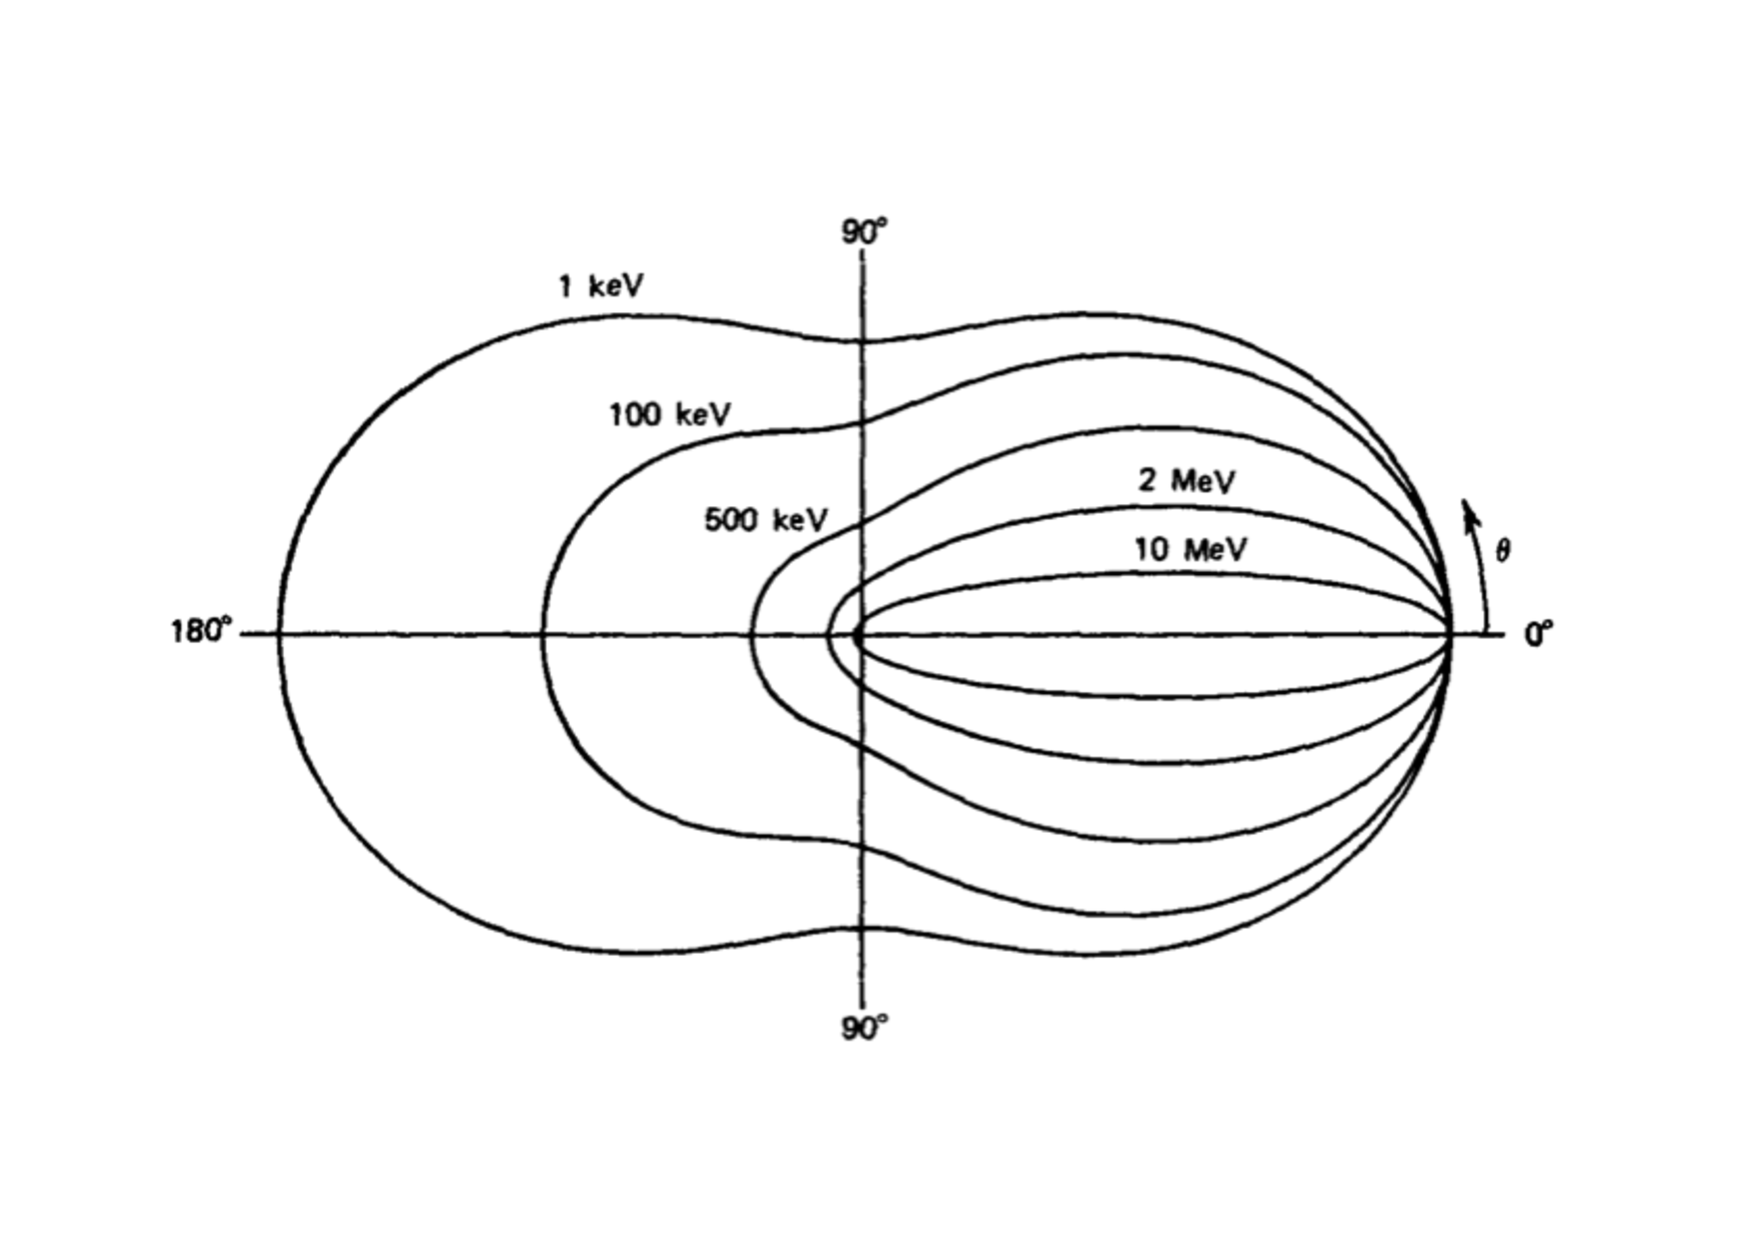
\includegraphics[width=0.8\textwidth]{03_GraphicFiles/chapter2_GammaCameras/ComptonPolar.pdf}
\caption{Polar plot of the number of photons (incident from the left side) Compton scattered into a unit solid angle at the scattering angle $\theta$, for the different indicated incident photon energies. In~\cite{Knoll2000}.}
\label{chap2::fig::ComptonAngCrossSection}
\end{figure}
 
As mentioned, the Compton cross section and energy transfer are calculated with the assumption of free electrons, but at very low incident photon energies such an assumption breaks down and the electronic binding energy $E_B$ affects the Compton interaction: the closer is the photon energy $h\nu$ to $E_B$, the larger is the deviation of the atomic cross section from the one calculated with the Klein-Nishina formula. Various theories have been developed to account for electronic binding energy effects and apply corrections on the Compton atomic cross sections~\parencite{Bergstrom1997}. It is worth to notice that for a given absorber Z, the binding energy correction is more significant at lower photon energies, and for a given initial energy $h\nu$, the binding energy correction is more significant at higher atomic number Z. The described binding energy effect is also referred to as \enquote{Doppler broadening}~\parencite{DuMond1928, DuMond1929}. 
   
If the photon incident energy exceeds twice the the rest-mass energy of and electron \myMarginnote{Pair production} $2m_ec^2 = $ 1.02~MeV, the production of an electron-positron pair in conjunction with a complete absorption of the photon becomes energetically possible. In practice, as shown in \figurename~\ref{chap2::fig::photonCrossSec},  the probability of such an interaction mechanism, referred to as pair production, remains very low until the gamma-ray energy approaches several MeV and therefore pair production is predominantly confined to high-energy photons. For $h\nu > 2m_ec^2$, energy and charge can be conserved even if pair production occurs in free space, but the conservation of linear momentum requires the Coulomb field of a collision partner (atomic nucleus or orbital electron). The photon, indeed, possesses momentum excess that is not absorbed by the electron-positron pair, and must be absorbed by the collision partner. When such an extra momentum is absorbed by the atomic nucleus, the recoil energy, as a result of the relatively large nuclear mass, is exceedingly small and the effect is described as the standard pair production: the incident gamma-ray disappears and is replaced by an electron-positron pair. When an orbital electron of the atom picks up the extra momentum, the recoil energy may be significant and determine the ejection of the orbital electron; in this case, the photon is absorbed and three particles leaves the interaction site, two electrons and a positron, in the so-called \enquote{triplet production}. A schematic representation of these two effects is given in \figurename~\ref{chap2::fig::pairprod}.

\begin{figure}[!htbp]
\centering
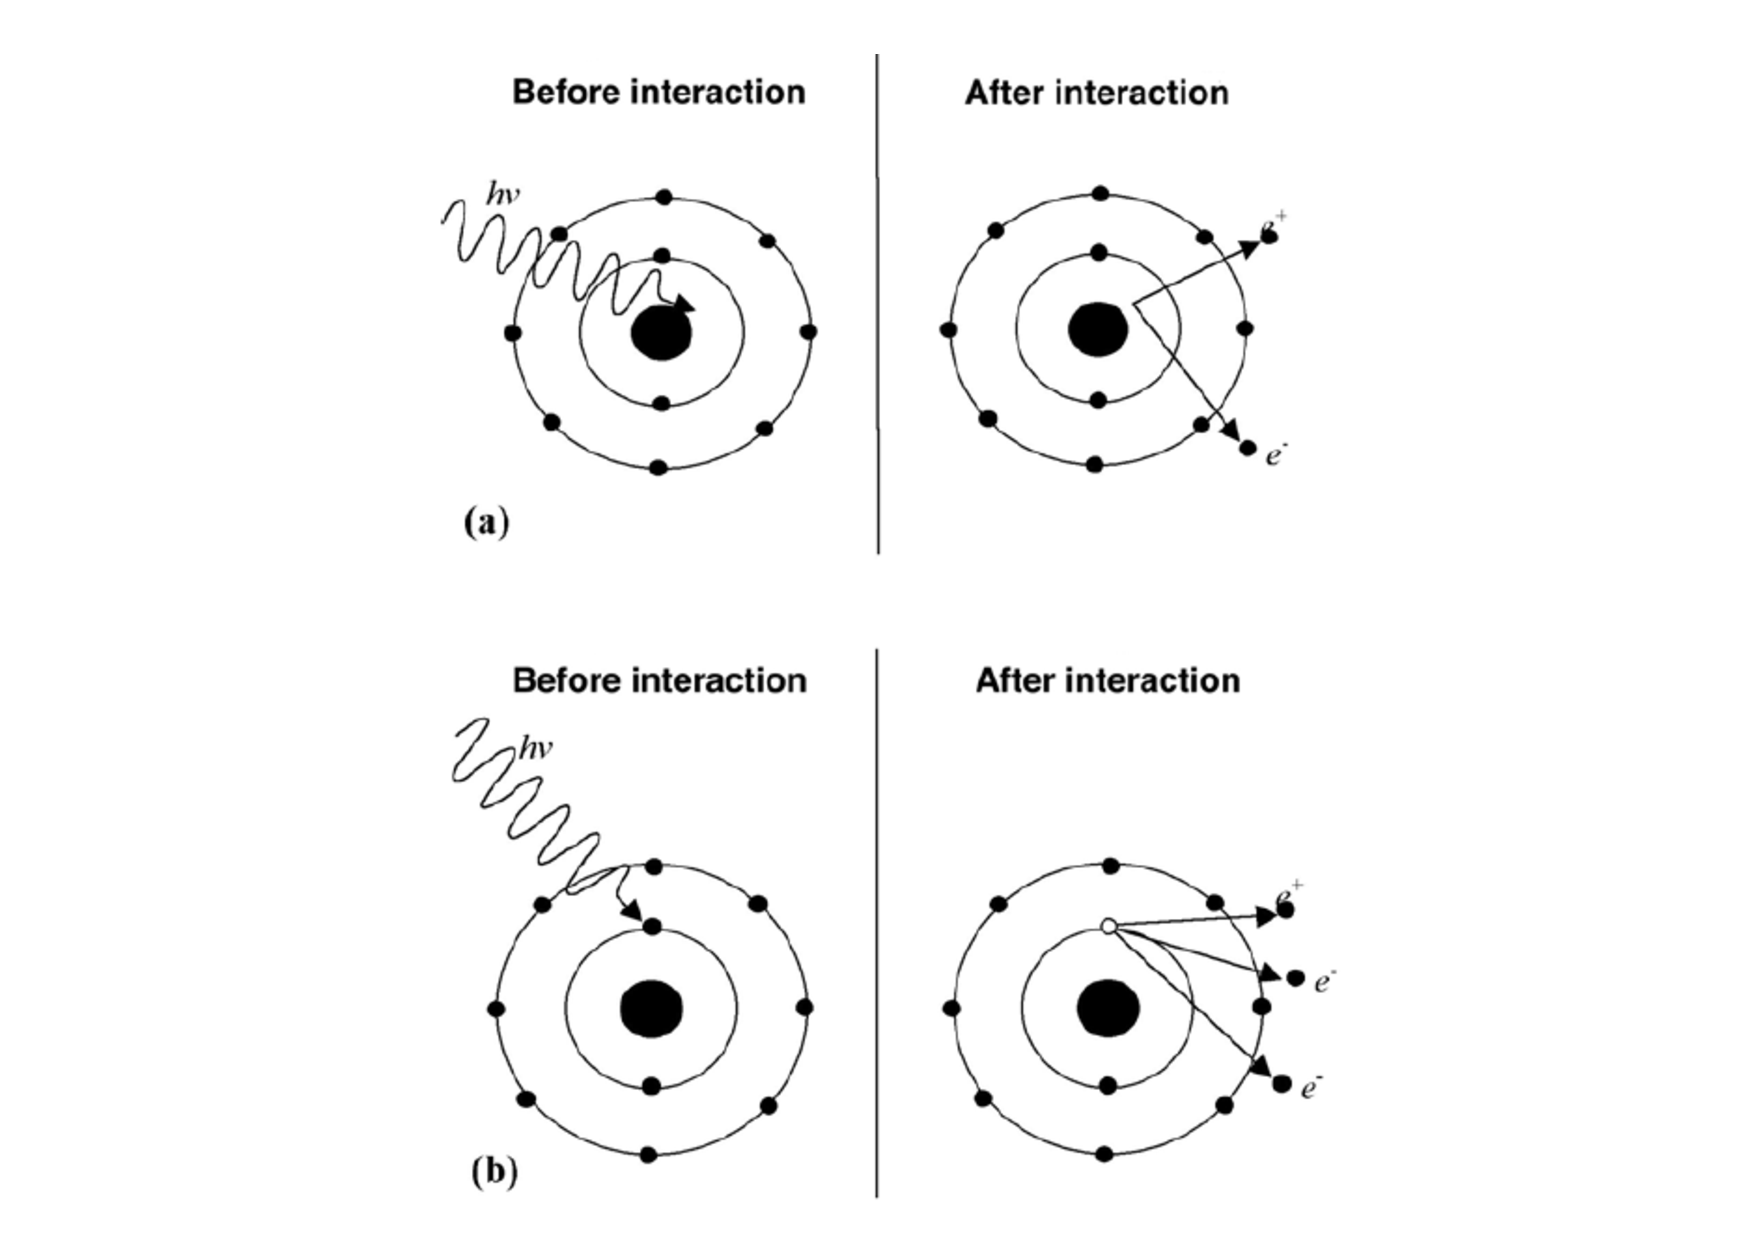
\includegraphics[width=0.9\textwidth]{03_GraphicFiles/chapter2_GammaCameras/pairProd.pdf}
\caption{Schematic representation of pari production (a) in the COulomb field of a nucleus and triplet production (b) in the Coulomb field of an orbital electron. In~\cite{Podgorsak2010}.}
\label{chap2::fig::pairprod}
\end{figure} 

The total kinetic energy transferred to the charged particles is the difference between the photon incident energy and twice the rest-mass energy of the positron-electron pair.
In both cases, because the positron will annihilate after slowing down in the absorbing medium, two annihilation photons are normally produced as secondary products of the interaction. 
No simple expression exists for the probability of pair production per nucleus, but its magnitude varies approximately as the square of the absorber atomic number Z, and it rises sharply with the photon energy. 

\begin{figure}[!htbp]
\centering
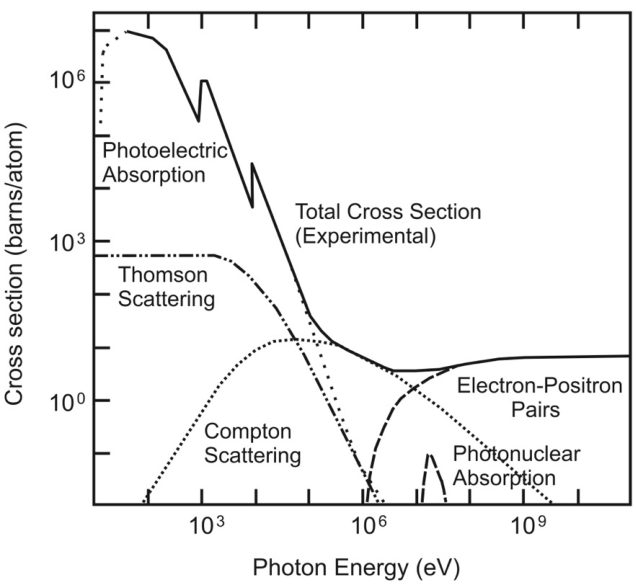
\includegraphics[width=0.8\textwidth]{03_GraphicFiles/chapter2_GammaCameras/Photon-energy-dependent-cross-sections-Cross-sections-of-the-photoelectric-absorption.png}
\caption{Cross sections of the photoelectric absorption, Thomson scattering, Compton scattering, pair production (electron-positron pairs), and photonuclear absorption for a copper absorber as a function
of the photon energy energy. In~\cite{Hermanss2013}.}
\label{chap2::fig::photonCrossSec}
\end{figure} 

The relative importance of the three described interaction processes for different absorber materials (Z) and gamma-ray energies ($h\nu$) are illustrated in \figurename~\ref{chap2::fig::relativePhotonInt}. Three areas are defined by the two solid lines in the plot, which indicates the energy/Z values for which the two neighboring effects have equivalent probability. 
 
\begin{figure}[!htbp]
\centering
\includegraphics[width=0.8\textwidth]{03_GraphicFiles/chapter2_GammaCameras/RelativePhotonInt.pdf}
\caption{Relative importance of the three major types of photon interaction in matter. The lines show the values of Z and $h\nu$ for which the two neighboring effects are just equal. In~\cite{Knoll2000}.}
\label{chap2::fig::relativePhotonInt}
\end{figure} 


If we now consider a photon beam interacting with a target, all the mentioned interaction processes removes gamma-ray photons from the beam either by absorption or by scattering away from the beam direction, and can be characterized by a fixed probability of occurrence per unit path length in the absorber. The sum of these probabilities is simply the probability per unit path length that the photon is lost and is referred to as \enquote{linear attenuation coefficient} $\mu$. Ther number of transmitted photons $I$ can be then expresses in terms of the number of incident photons in the beam $I_0$ as a function of the linear attenuation coefficient and the absorber thickness $t$, as shown by equation~\ref{chap2::eq::attenuation}.

 \begin{equation}
\frac{I}{I_0} = e^{-\mu t}
\label{chap2::eq::attenuation}
\end{equation} 

The average distance traveled by the a photon of the beam in the absorber before an interaction takes place is called \enquote{mean free path} $\lambda$, and is the reciprocal of the linear attenuation coefficient. In solids, for common gamma-ray energies, $\lambda$ can vary in the range between few millimeters to tens of centimeters. 
A more widely used parameter is the \enquote{mass attenuation coefficient} $\mu_{\rho}$, which normalize the linear attenuation coefficient to the absorber density $\rho$ (equation~\ref{chap2::eq::massAttenuation}).

\begin{equation}
\mu_{\rho} = \frac{\mu}{\rho}
\label{chap2::eq::massAttenuation}
\end{equation} 

If the mass attenuation coefficient is used, the convenient concept of mass thickness is also introduced, corresponding to the product of the absorber thickness $t$ by its density $\rho$ and generally measured in mg/cm$^2$. For compound and mixtures, the mass attenuation coefficient is approximated by a summation of a weighted average of its constituent, as expressed in equation~\ref{chap2::eq::massAttCoeffCompoud}.

 \begin{equation}
\mu_{\rho} = \sum_i{w_i\frac{\mu_i}{\rho}}
\label{chap2::eq::massAttCoeffCompoud}
\end{equation} 

with $w_i$ the proportion by weight of the i-th constituent, and $\mu_i/rho$ its mass attenuation coefficient. The attenuation coefficients have specific values for a given photon energy $h\nu$ and absorber atomic number Z, and are tabulated on the \gls{nist} database according to the calculations in~\cite{Seltzer1993}.


\section{Ion range monitoring with secondary gamma rays}\label{chap2::sec::GammaIonRange}

Among the secondary radiations produced during particle therapy treatments, gamma rays are probably the most extensively studied for range verification purposes. Gamma rays are emitted in relaxation processes of atoms excited by the beam nuclear interactions and as result of the annihilation of positrons produced by beam-induced positron emitting isotopes. In both cases, the emission profiles correlate to the ion path in matter, and the profile fall-off allows to locate the Bragg peak position. 

In the following, the developed methods exploiting these two ion range signatures are described.

\subsection{Range verification with Positron Emission Tomography}\label{chap2::subsec::PETrangeVerif}

As explained in section~\ref{chap1::subsubsec::ionInteractions}, the fragmentation processes involving target nuclei during proton therapy irradiation and both projectile and target nuclei in case of heavier ion beam therapy, can produce radioactive isotopes. In particular, $\beta^+$ emitting fragments are of significant interest for range verification purpose. Table~\ref{chap2::tab::petIsotopes} shows the main reaction channels and relative isotopes produced along a proton beam path in tissue. More details about the most relevant reaction channels and their characteristics (energy threshold, isotope decay constant, maximal kinetic energy of the emitted positrons), can be found in~\cite{Oelfke1996}. Additional channels and isotopes are produced during carbon ion irradiation, given the possible projectile activation. 

\begin{table}[!htbp]
\centering
\caption{Proton-nuclear reaction channels and relative positron emitters produced in human tissues. Table reproduced from~\cite{Espana2011b}.}
\label{chap2::tab::petIsotopes}
\resizebox{\textwidth}{!}{%
\begin{tabular}{llcc}
\toprule
\rowcolor{myColorMainA!20} 
\textbf{Target}& \textbf{Nuclear reaction channel} & \textbf{$\beta^+$ isotopes} & \textbf{Half-life} \\
\midrule
C & $^{12}$C(p, pn)$^{11}$C, $^{12}$C(p, p2n)$^{10}$C & $^{10}$C, $^{11}$C & 19.29~s, 20.33~min\\
N & $^{14}$N(p, 2p2n)$^{11}$C, $^{14}$N(p, pn)$^{13}$N, $^{14}$N(p,n)$^{14}$O & $^{13}$N ($^{11}$C, $^{14}$O) & 9.96~min \\
O & $^{16}$O(p, pn)$^{15}$O, $^{16}$O(p, 3p3n)$^{11}$C, $^{16}$O(p,2p2n)$^{13}$N, $^{16}$O(p,p2n)$^{14}$O, $^{16}$O(p,3p4n)$^{10}$C   &  $^{14}$O, $^{15}$O, ($^{11}$C, $^{13}$N)& 70.61~s, 122.24~s\\
P & $^{31}$P(p, pn)$^{30}$P&$^{30}$P & 2.50~min\\
Ca & $^{40}$Ca(p, 2pn)$^{38}$K & $^{38}$K & 7.64~min\\
\bottomrule
\end{tabular}}
\end{table}    

\begin{figure}[!htbp]
\centering
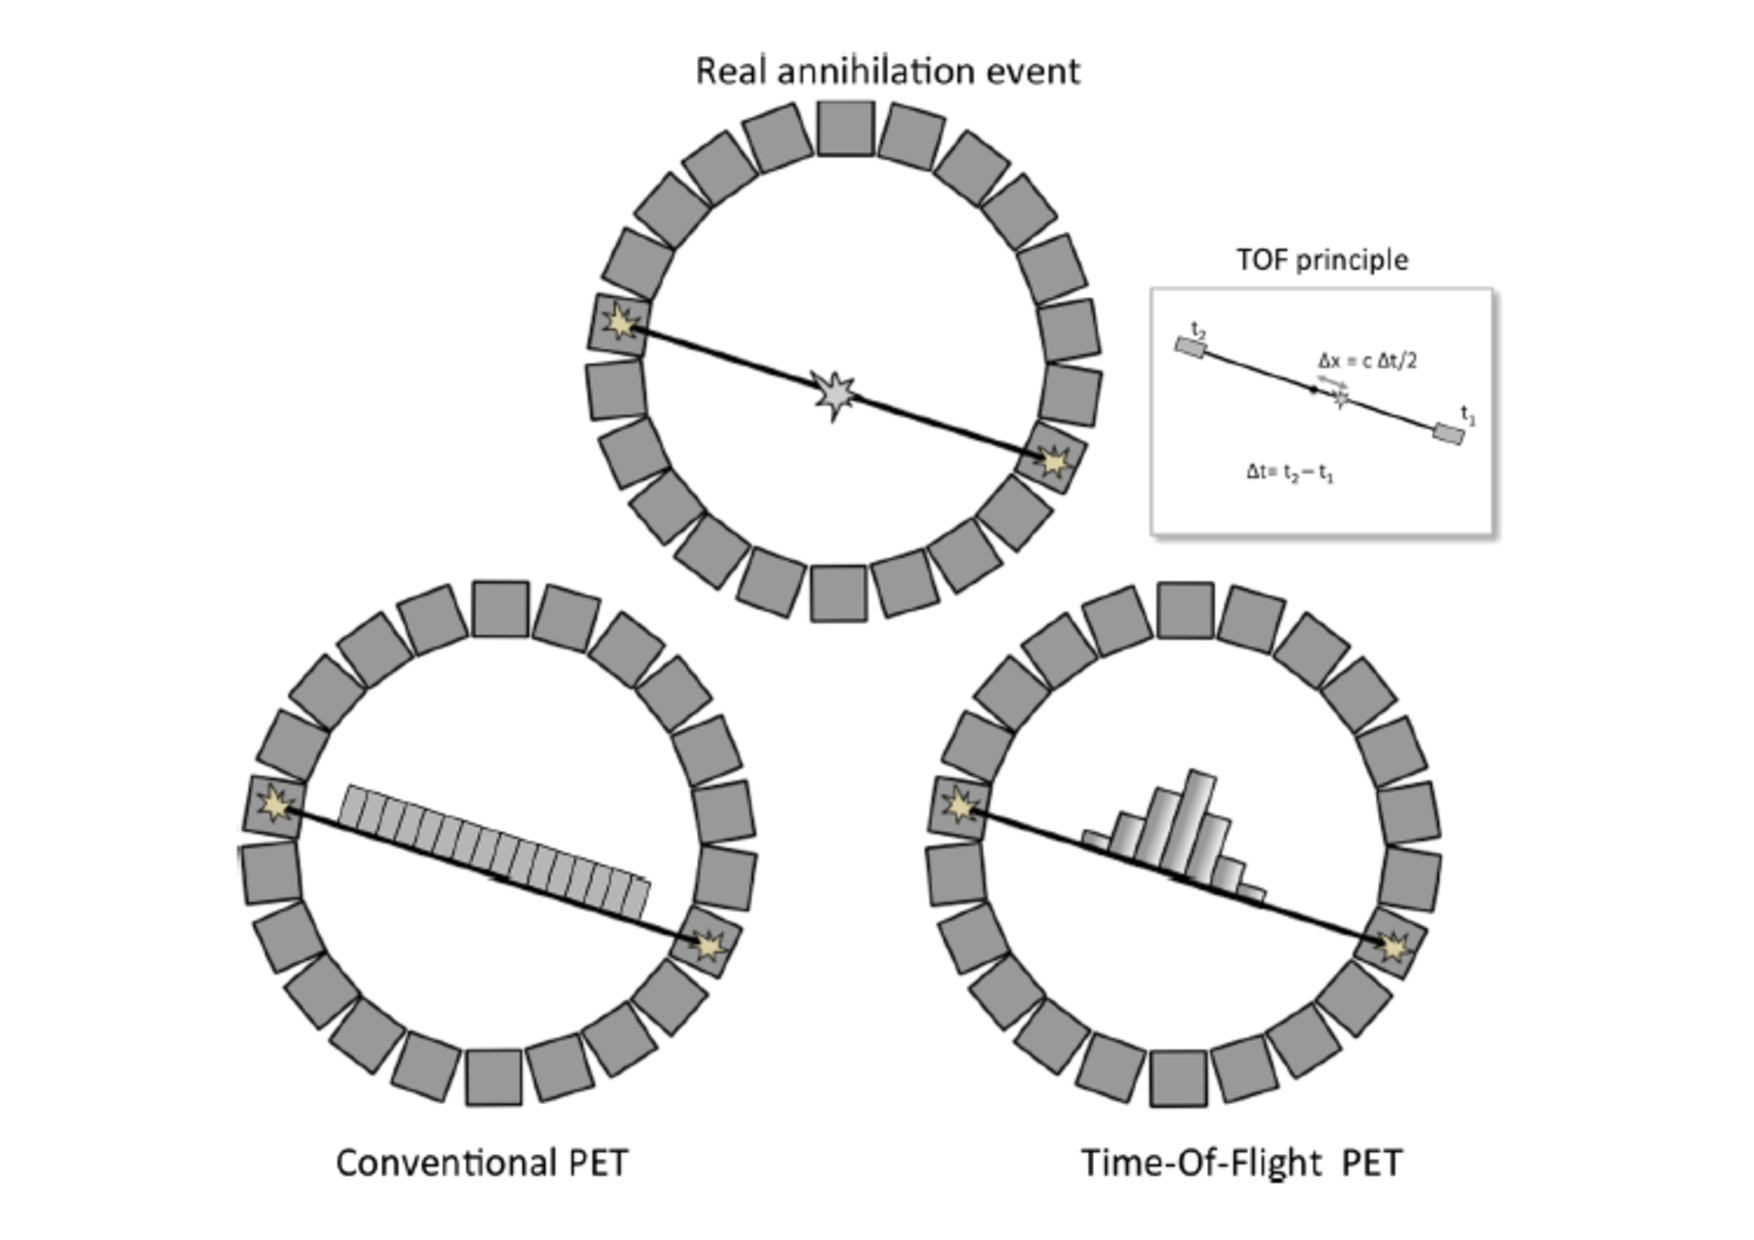
\includegraphics[width=0.8\textwidth]{03_GraphicFiles/chapter1_Introduction/PET_concept.pdf}
\caption{Schematic representation of the \gls{pet} technique principle. In the top figure, a standard real annihilation event is presented, while in the bottom line the principle of conventional and \gls{tof}-\gls{pet} are compared. In~\cite{Vandenberghe2016}.}
\label{chap2::fig::PETconcept}
\end{figure}   

\figurename~\ref{chap2::fig::PETconcept} (top) shows the concept of the \gls{pet} detection technque. The emitted positrons annihilate with human tissue electrons after traveling few mm distances, and 511~keV back-to-back photons are produced and can be detected in coincidence with \gls{pet} machines. The spatial distribution of the $\beta^+$ decay points can be then obtained via the reconstruction of the so-called \enquote{lines of response} connecting the two detected photons, and it correlates, even if not directly, to the dose profile. \figurename~\ref{chap2::fig::PETrangeProf} shows the one-dimensional $\beta^+$ activity profiles along the beam axis for various incident beam types impinging on a \gls{pmma} target. The positron emitter distribution dependence on the beam nature clearly emerges from these profiles, but a form of indirect correlation with the dose profile distal edge is always verified. In particular, a remarkable difference exists between light ions (protons, $^3$He and $^7$Li), for which the induced activity is almost only due to target residuals, and heavier ones ($^{12}$C and $^{16}$O), with a considerable contribution also coming from projectile fragmentation sub-products, which concentrate near the end of the range, explaining the activity peak. The investigation of the correlation between delivered dose and $\beta^+$ detected activity must face several issues, as highlighted in~\cite{Parodi2004}, mainly connected to the difficulty to retrieve quantitative information from \gls{pet} images and to wash-out effects. Long-lived positron emitters, indeed, can be transported away from the production point by blood flow and metabolic processes, affecting the precision of the obtained images. This effect has been deeply studied experimentally at \gls{himac} with rabbit tissues and Anger-type scintillation cameras~\parencite{Mizuno2003, Tomitani2003}, and, more recently, at \gls{gsi} with $^{12}$C beams~\parencite{Fiedler2008}. A reduction of a factor up to 1.5 in the precision of the range determination due to wash-out processes is reported, and a correlation between biological half-life and local dose has been verified and used in simulation to improve the quality of \gls{pet} images. Although several research efforts have been dedicated to improve the precision of the dose recovery from $\beta^+$-emitter distributions~\parencite{Parodi2006, Parodi2007, Parodi2010}, the only feasible solution for the monitoring of dose delivery is the comparison of measured distributions to simulated ones~\parencite{Ponish2004}. These Monte Carlo simulations are based on the planning \gls{ct} scan, the irradiation scheme, the detector geometry, the imaging procedure; deviations in the delivered dose caused by patient positioning or anatomical modifications can be detected, mainly because they are reflected in changes in the maximum particle range in the target tissues. Thus, the main quality criterion of the \gls{pet} monitoring method is the precision in the measurement of range shifts with respect to the predicted ones~\parencite{Fiedler2010}. The accuracy of the reference simulated activity distribution has advanced in the last years, but it is still limited by the lack of underlying cross-sectional data, the not perfect knowledge of the elemental composition of the patient and the complex prediction of metabolic wash-out processes. Complementary imaging modalities can give fundamental contributions to the simulation predictions: for example, the use of supplemental \gls{mri} data has been proposed to better analyze local wash-out effects. In addition to this, the implementation of hybrid \gls{pet}-\gls{ct} systems, preferably with dual-energy \gls{ct}, would improve the conversion of \gls{ct} information to the material composition needed for the \gls{pet} simulations~\parencite{Landry2013}.  

\begin{figure}[!htbp]
\centering
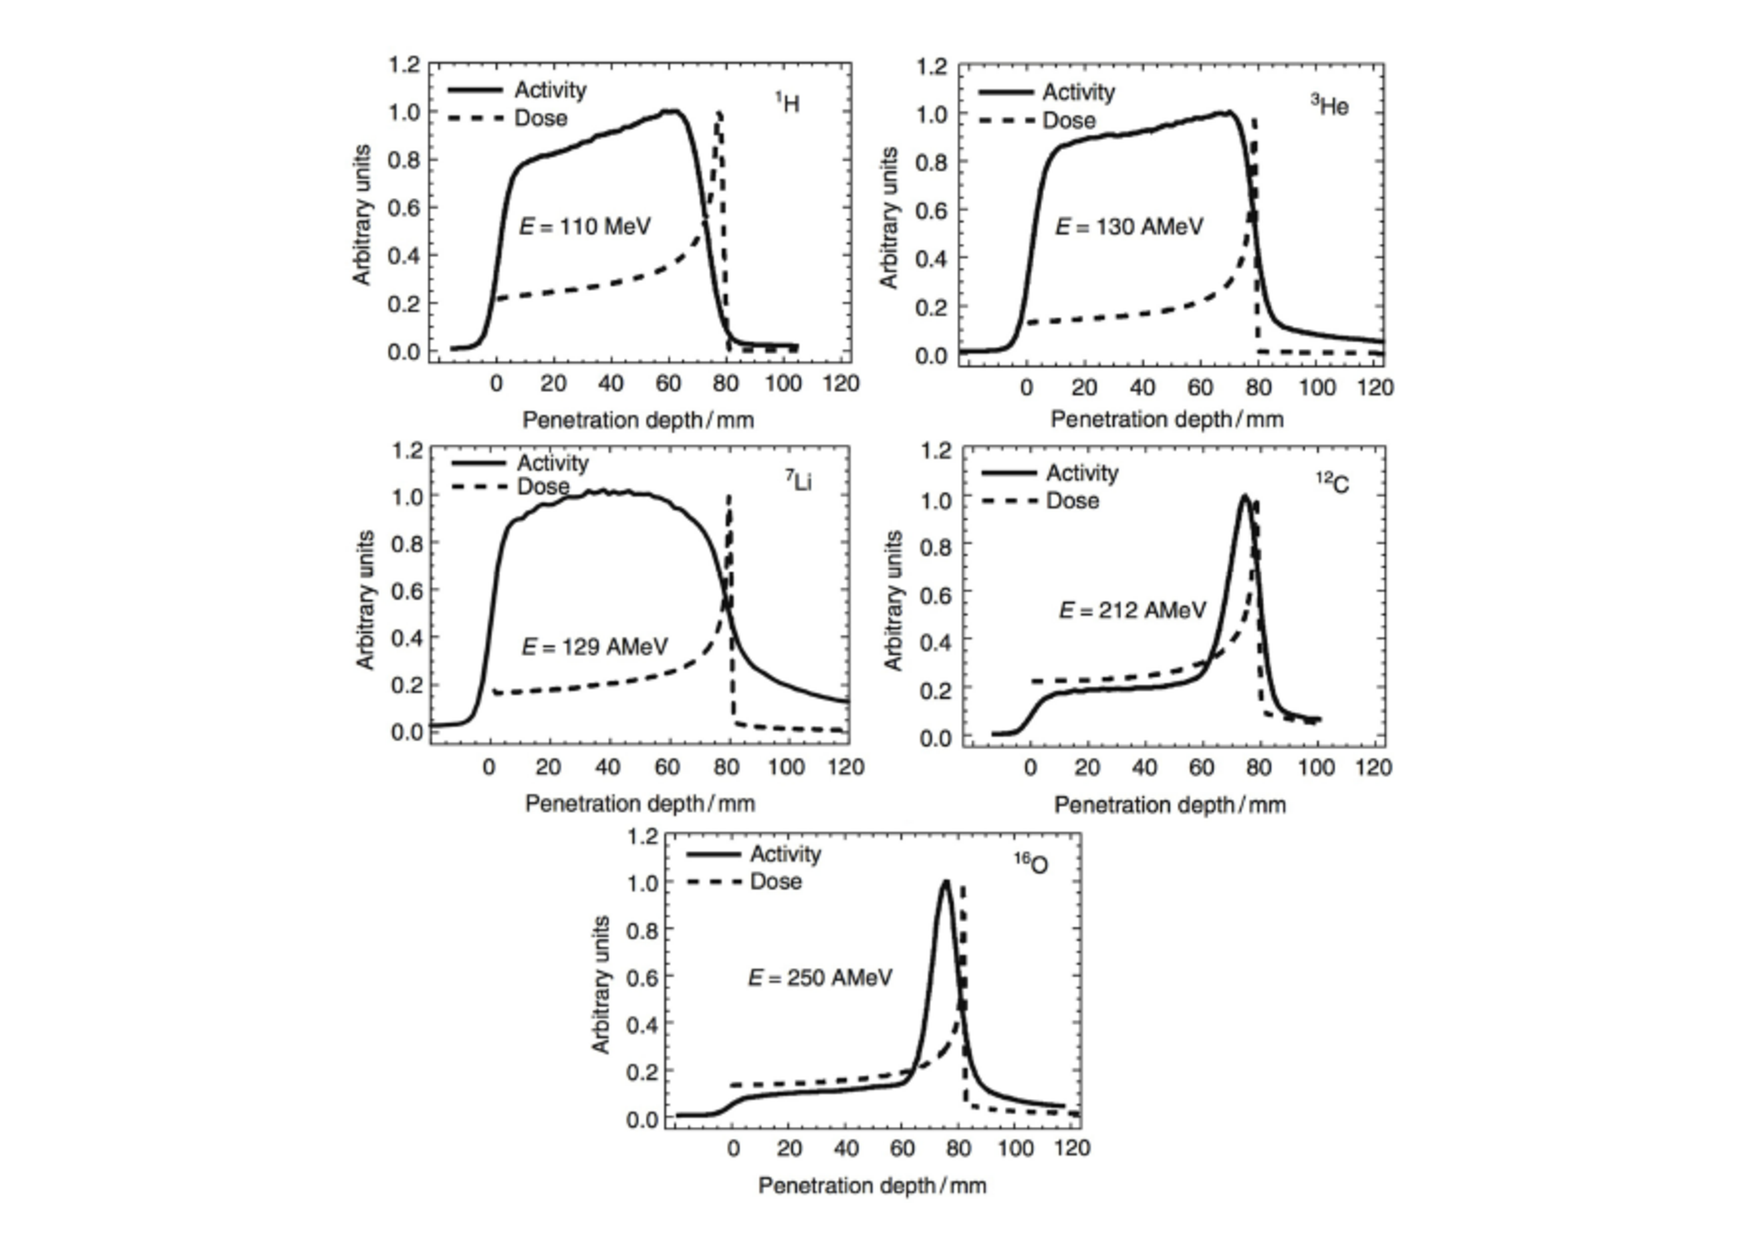
\includegraphics[width=0.98\textwidth]{03_GraphicFiles/chapter1_Introduction/PETrangeProf.pdf}
\caption{$\beta^+$ activity profiles for various ion beams impinging on a \gls{pmma} thick target. The depth-dose profiles are also shown in dashed lines for comparison. In~\cite{Fiedler2012}.}
\label{chap2::fig::PETrangeProf}
\end{figure}   

The \gls{pet} data acquisition can be performed following three main strategies:
\begin{itemize}
\item In-beam data acquisition: the \gls{pet} system is integrated in the beam delivery system and the data acquisition is performed during or immediately after irradiation in the treatment room. In synchrotron facilities, a further solution is represented by acquisitions in the time between different spills, while for cyclotrons data-taking during beam extraction has been explored and seems feasible~\parencite{Kraan2014}. On one hand, this method is advantageous because it allows detecting short-lived isotopes, thus increasing the available statistics, and reducing the effects of biological processes. Moreover, the patient position does not change with respect to the treatment. On the other hand, the integration of \gls{pet} scanners in the treatment site can be costly and cause limitations on the detector geometry affecting detection efficiency and, consequently, image quality. The scanner should not be directly exposed to the beam in order to avoid damage and activation of active modules and electronics, and at the same time it should allow enough degrees of freedom for the patient table. The need of an opening for the beam portal typically results in the choice of planar dual-head configurations.
\item In-room data acquisition: the installation of commercial full-ring \gls{pet} scanners in the treatment room, but not directly on the beam line, allows the so-called \enquote{in-room} data acquisitions quickly after the end of the treatment irradiation. This solution leads to longer treatment room occupation, because some minutes of imaging time is required to gain enough statistics, but allows one to use commercial machines, less expensive and more efficient than custom integrated scanners designed for in-beam applications. Moreover, patient positioning issues are minimized by the limited movements and signal wash-out is reduced.
\item Off-line data acquisition: if the patient has to be transported out of the treatment room for the \gls{pet} scan, the implemented strategy is classified as \enquote{off-line}. The limited cost and treatment occupation time are probably the only advantages of this method, which suffers from relevant signal decay and wash-out processes given the long time between the end of the irradiation and the beginning of the \gls{pet} scan. Off-line images predominantly show activity from isotopes whose half-life is comparable or longer then the transportation and setup time, thus it is mainly restricted to $^{11}$C (half-life longer than 20 minutes), produced in relative small amount in proton therapy, more abundant in carbon treatments. The reduced number of available decays requires longer acquisition time with respect to in-beam and in-room solutions, which further enhance the effect of metabolic processes. The patient repositioning issues also contribute to the image quality degradation. 
\end{itemize}
A schematic view of the three \gls{pet} acquisition modalities is presented in \figurename~\ref{chap2::fig::PETmodes}. As mentioned in the three data acquisition modality description, the counting statistics is one of the fundamental parameters to be studied for the design of \gls{pet} monitoring solutions. It can be estimated as the integral of the decay curve shown in \figurename~\ref{chap2::fig::PETactDistr}, where the time intervals corresponding to the three acquisition strategies are separated. The curve is based on measurements performed at \gls{gsi} during therapeutic irradiation with carbon ions; an in-beam solution has been adopted, with 40~s additional data taking time after the irradiation. The in-room selected window lasts 3 minutes, and for the off-line case, long-time measurements of one patient have been used~\parencite{Fiedler2008b}. If 100\% is assigned to the number of registered true events in the in-beam condition, 50\% is estimated for the in-room solution and 58\% for the off-line data taking~\parencite{Shakirin2011}. It is then clear that off-line solutions are severely challenged by the extremely low signal, considerably lower with respect to the standard application of the employed commercial scanners (down to average activity values of few tens of Bq/ml~\parencite{Bauer2013}).
The scanner geometry is another fundamental parameter to be considered: as mentioned, the chosen data-acquisition strategy determines the scanner design. In-room and off-line solutions can make use of commercial full-ring systems, with a complete field of view. In addition to this, modern combined \gls{pet}-\gls{ct} scanners enable an accurate co-registration of treatment and imaging position, so that the unavoidable patient movement due to transportation and repositioning can be partially corrected. The geometrical constraints imposed by in-beam integrated solutions cause reduced efficiency and restricted field-of-view, which are reflected in image artifacts~\parencite{Crespo2006}, particularly significant in the imaging of large tumor objects. Improvement can be provided by \gls{tof}-\gls{pet} detectors~\parencite{Crespo2007, Surti2011}, as discussed below.
In~\cite{Parodi2015} the author highlights how the first historical attempts to implement \gls{pet} particle therapy monitoring, described in the following, have not relied on optimized instrumentation for the peculiar application. Anyway, the promising results obtained by several groups encouraged dedicated investigations which are leading to substantial improvements of such a technique in the last years. In particular, the application of gamma detectors with depth-of-interaction capability, also studied for standard diagnostics applications, has demonstrated its effectiveness in correcting parallax artifacts in the reconstructed images; improvements in data acquisition and synchronization with the accelerator radio-frequency offer the possibility of including the signal detected during the beam-on time for in-beam solutions, thus increasing the counting statistics and reducing the acquisition time; new adapted geometries, such as the Japanese OpenPET system~\parencite{Tashima2012, Yamaya2008}, recently finalized in its upgraded version~\parencite{Yamaya2017}, offer higher-efficiency alternatives to standard dual-head systems. 
It is worth to dedicate particular attention to the already mentioned \gls{tof}-\gls{pet}, deeply studied in the last years, which already demonstrated improved imaging capabilities with respect to standard scanners. The measurement of the detection time of each of the two photons helps, through the calculation of the arrival time difference, in restricting the emission point along the reconstructed line of response and thus also in rejecting part of accidentals. In standard \gls{pet}, the three-dimensional reconstruction relies on the superposition of several lines of response and on filtered back-projection algorithms. The time information adds a second dimension to the line of response reconstruction, with the localization of the interaction point in a few cm along the line, depending on the detector time resolution. For example, a coincidence timing resolution of 600 ps \gls{fwhm} translates to a position uncertainty of 9 cm \gls{fwhm}. In~\figurename~\ref{chap2::fig::PETconcept} (bottom line), the \gls{tof}-\gls{pet} principle is sketched and compared to the conventional \gls{pet} detection scheme. 
The potential benefits of \gls{tof} information in \gls{pet} image reconstruction were already understood since the early stage of its development for diagnosis purpose, and the first \gls{tof}-\gls{pet} systems were built already in the 1980s in the US~\parencite{Gariod1982}. They were based on \gls{csf} or \gls{baf2} scintillators, the best available at the time in terms of time resolution, but their spatial performance and sensitivity were poor with respect to conventional \gls{pet} scanners. The improvements in scintillating material as well as in \gls{pm} performance and reliability allowed for the first commercial proposal of a \gls{tof}-\gls{pet} scanner only in 2006, by Philips~\parencite{Surti2007}. The development of \gls{tof}-\gls{pet} machines is strongly connected to their application in diagnosis, and further details will be given in section~\ref{chap2::subsec::PET_NM}. As for particle therapy monitoring application, the \gls{tof} technique applied to \gls{pet} can be used to partially reverse the effects caused by non-complete angles of in-beam data collection~\parencite{Crespo2006}, and in general to improve the image quality. Various groups are developing detector solutions for clinical implementation of such a technique; some of them have already been tested on beam with promising results. They will be described in more details in the following, after a brief historical overview of the \gls{pet} application in particle therapy quality assurance. 

\begin{figure}[!htbp]
\begin{subfigure}[t]{.49\textwidth}
\centering
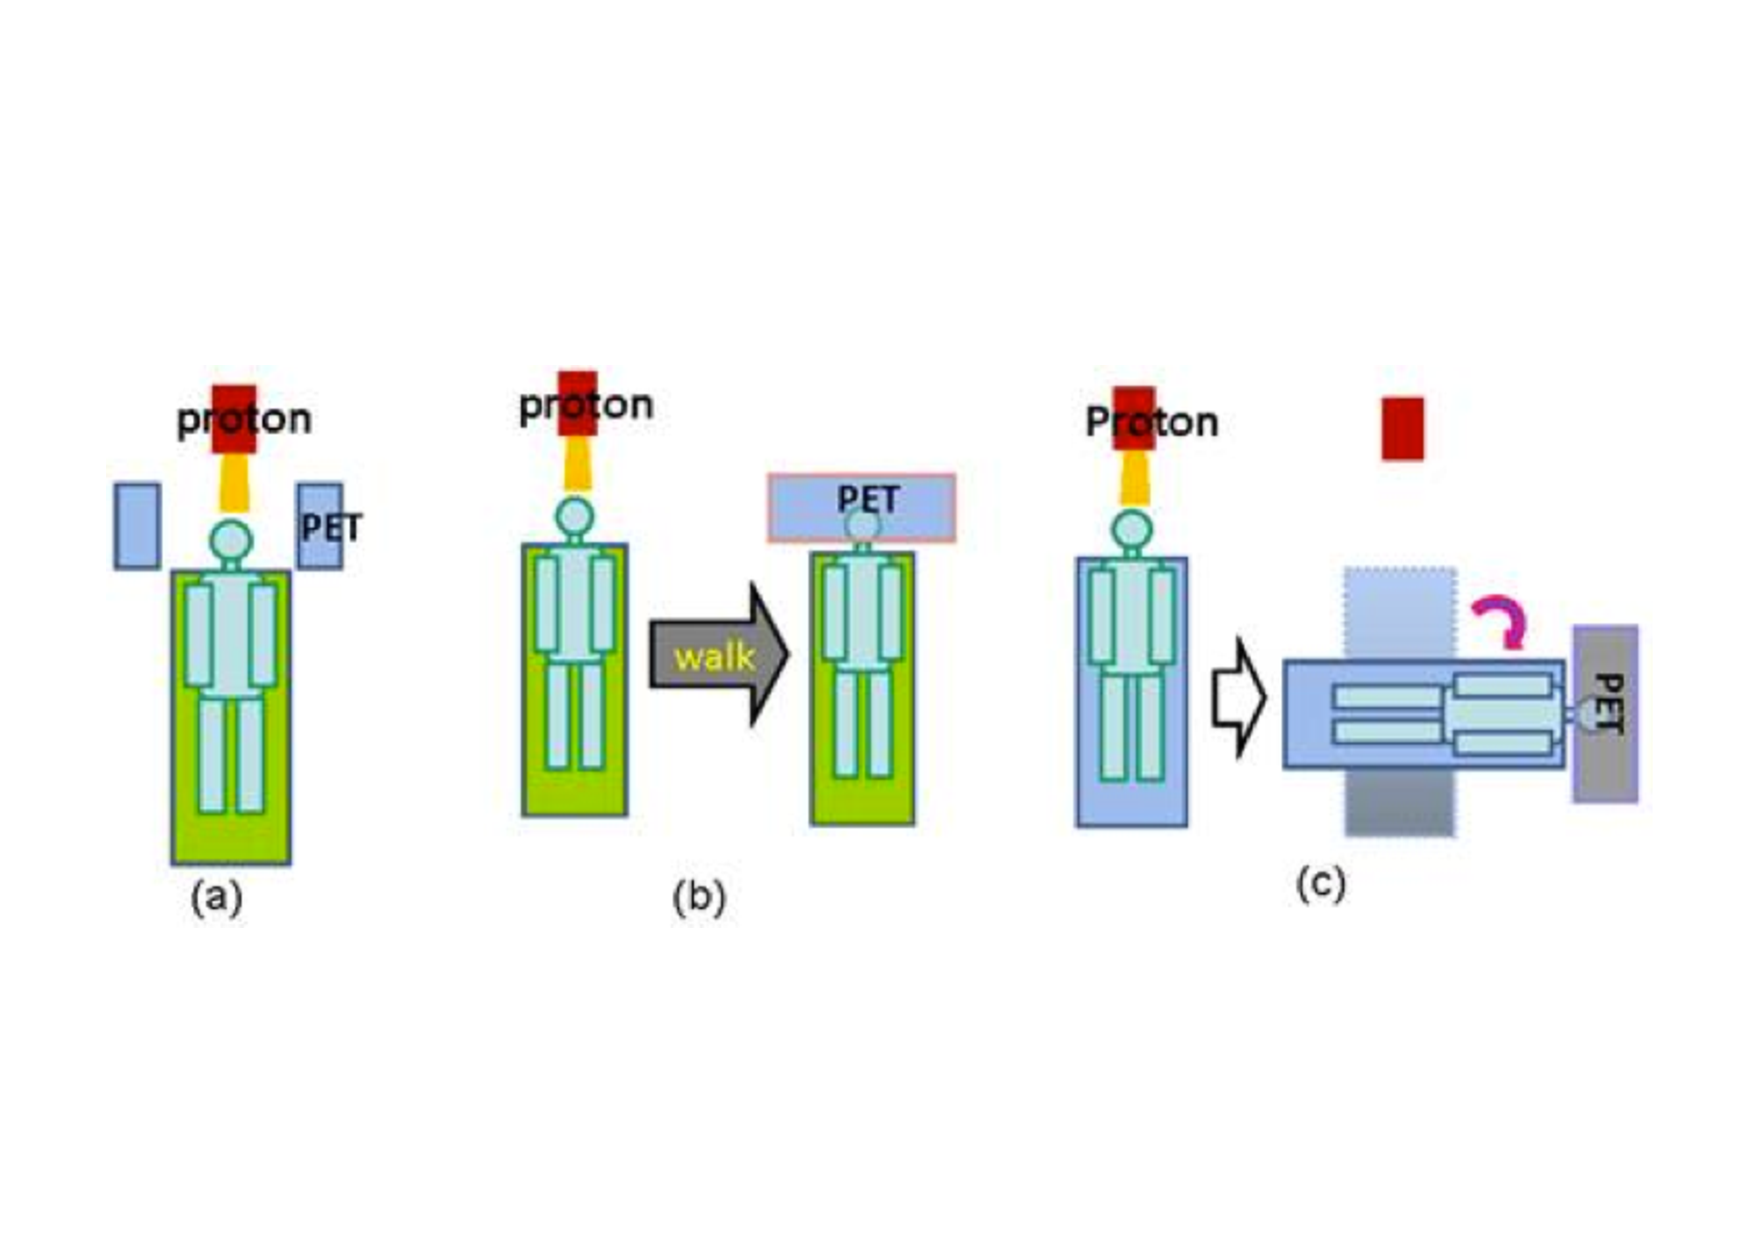
\includegraphics[width=0.98\linewidth]{03_GraphicFiles/chapter1_Introduction/PETmodes.pdf}
\caption{Schematic view of the three \gls{pet} configurations for the application in ion range monitoring. Form left to right: in-beam, off-line and in-room \gls{pet}. In~\cite{Zhu2013}.}
\label{chap2::fig::PETmodes}
\end{subfigure}
\begin{subfigure}[t]{.49\textwidth}
\centering
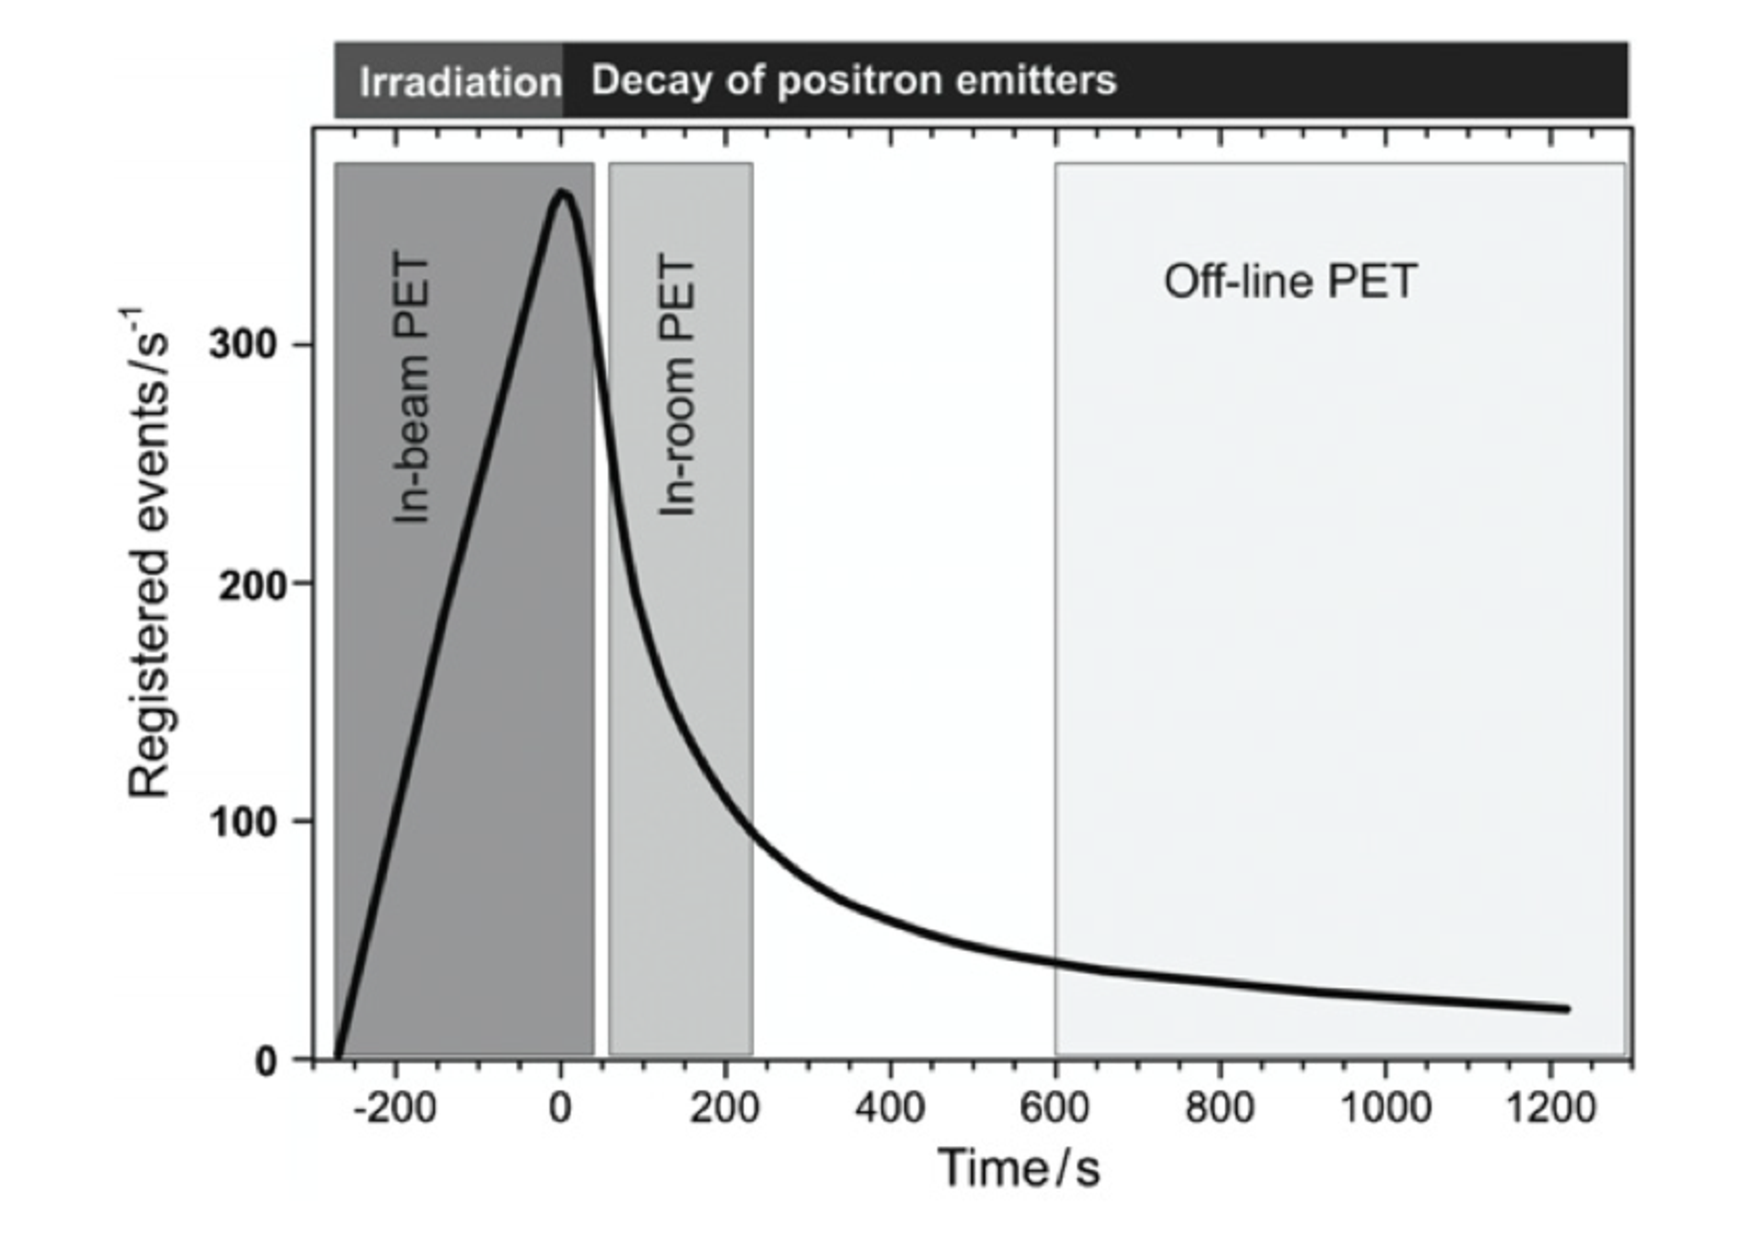
\includegraphics[width=0.92\linewidth]{03_GraphicFiles/chapter1_Introduction/PETactDistr.pdf}
\caption{\gls{pet} registered events as a function of time corresponding to the measurement of one field during
irradiation and up to 20 minutes after irradiation. The time intervals corresponding to  in-beam, in-room, and off-line \gls{pet} measurements are highlighted. In~\cite{Shakirin2011}.}
\label{chap2::fig::PETactDistr}
\end{subfigure}
\caption{The application of the \gls{pet} technique to the monitoring of ion range in particle therapy includes three possible modalities: in-beam, in-room and off-line \gls{pet}, represented in the scheme in (a). The amount of registered events depends on the created positron emitter half-life, and thus on the implemented modality, as shown by the histogram in (b).}
\label{chap2::fig::PETmodalities}
\end{figure} 

As emerges from the above paragraphs, \gls{pet} is probably the most extensively studied technique for online beam range verification and is at present the only method clinically implemented~\parencite{Enghardt2004, Yamaya2018}. The first published proposal of using \gls{pet} for range verification in particle therapy dates back to 1975~\parencite{Bennett1975}. In the next years, further suggestions were connected to pion~\parencite{Goodman1986, Shirato1989} and neutron therapy~\parencite{Vynckier1989}, but the actual clinical implementation was pioneered in the context of heavy ion therapy at \gls{lbl}~\parencite{Llacer1979, Chatterjee1981}. The original idea was to verify the correctness of $^{20}$Ne ion therapy treatment plans by delivering a low dose $\beta^+$ emitting ion beam (e.g. $^{19}$Ne) prior to the treatment and measuring its range via \gls{pet} imaging of the emitted photons; before the regular treatment with stable beams. Pilot experiments were conducted with a planar \gls{pet} camera based on two blocks of \gls{bgo} crystals, including measurements in a live dog~\parencite{Llacer1984b}. The experimental data showed interesting results, even if the use of a passive beam shaping system determined a significant activation of the \gls{bgo} camera (mainly due to neutrons) and, thus, a substantial noise level. Analog investigations using radioactive ion beams ($^{15}$O, $^{17}$F, $^{19}$Ne) were carried out in the nineties at \gls{gsi} with various \gls{pet} cameras~\parencite{Pawelke1996}, and further developments of this technique were obtained at the \gls{himac} facility~\parencite{Iseki2004, Kitagawa2006}, where a dedicated line was set up for radioactive beam based treatments~\parencite{Urakabe2001, Kanazawa2002}. The \enquote{autoactivation} process~\parencite{Tobias1971} described above (i.e. the production of radioactive nuclei in the target by incident beam of stable ions) makes anyway possible the implementation of \gls{pet} monitoring techniques on standard high-energy beams, and the first clinical implementation of such  technique was launched at \gls{gsi} in 1997, after the tests with radioactive beams mentioned above and fragmentation studies conducted with $^{12}$C, $^{16}$O, $^{20}$Ne beams on a \gls{pmma} target~\parencite{Enghardt1992}. An in-beam \gls{pet} system was designed and installed into the treatment room and has been employed routinely for monitoring the irradiation of more than 440 patients (mainly suffering from head-and-neck cancer), with data acquisitions performed in the pause of pulsed beam delivery. This experience proved how \gls{pet} is a valuable tool for particle therapy quality assurance~\parencite{Enghardt2004}. In parallel to these developments in Germany, an off-line solution was implemented at \gls{nirs} with a commercial full-ring volumetric scanner, but it was not used in clinics. As previously explained, notwithstanding the lacking peak structure in the activity profile (cf. \figurename~\ref{chap2::fig::PETrangeProf}), also proton irradiation therapy can be monitored by \gls{pet} scanners. Various detailed studies investigated its feasibility and performance in the nineties~\parencite{Litzenberg1992, Paans1993, Oelfke1996, Litzenberg1999}. Two groups worked in parallel on clinical studies of \gls{pet} monitoring in proton therapy. In Japan, a dual-head \gls{pet} scanner has been installed at the National Cancer Center, Kashiwa~\parencite{Nishio2006}: it is based on high-resolution \gls{bgo} detector components and integrated in the proton gantry. The measurements are collected immediately after irradiation (in-room solution), mainly due to the considerable radiation background during the continuous beam delivery and the passive beam shaping. The satisfactory results led to the implementation of a daily \gls{pet} workflow, which allowed the research group to follow the anatomical changes of the patient during the treatment progress and correct the treatment planning. The test of this method included 48 patients suffering from head-and-neck, liver, lung, prostate and brain tumors~\parencite{Nishio2010}. In the US, at the \gls{mgh}, Boston, a pilot clinical study was performed with an off-line solution which made use of a commercial full-ring scanner~\parencite{Parodi2007}. The \gls{pet} scan was performed about 20 minutes after proton irradiation. The off-line approach has been deeply studied in the same context in those years, and compared to in-beam \gls{pet} solutions in cyclotron and synchrotron based scenarios~\parencite{Parodi2008, Knopf2011}. The advantage in terms of available statistics for in-beam solutions has been measured: the ratios between the amount of physical decays available for in-beam and off-line detection range from 40\% to 60\% for cyclotron-based facilities, to 65\% to 110\% (carbon ions) and 94\% to 166\% (protons) at synchrotron-based facilities~\parencite{Parodi2008}. The in-room solution has also been explored at the same institution, with an acquisition time reduced to less than 5 minutes thanks to the higher sensitivity with respect to the off-line modality~\parencite{Zhu2011}.  
At \gls{hit}, in Germany, both an in-beam~\parencite{Sommerer2009}, and an off-line solution~\parencite{Bauer2013} have been tested, while alternative off-line solutions have been implemented in Japan~\parencite{Hishikawa2002} and US~\parencite{Hsi2009}. 
With the aim of extending the field of view and thus enhancing the sensitivity of in-beam \gls{pet} designs, Japanese researchers proposed the already mentioned OpenPET as a new geometrical solution. Its first-generation prototype is composed of two complete rings, with the beam port between the two~\parencite{Yamaya2008, Yamaya2009} and the possible implementation of an integrated \gls{ct}. A more efficient geometry has been proposed some years later, consisting of a single-ring which can provide an accessible and observable open space with higher sensitivity and reduced number of detectors compared to the previous generation one~\parencite{Tashima2012}. The ring is cut at a slant angle in order to be disposed at a certain angle with respect to the beam line, but maintain parallel detector modules orientation. A similar solution was proposed in~\cite{Crespo2006}, but with a conventional \gls{pet} ring with an oblique orientation with respect to the beam direction (\enquote{slant \gls{pet}}). A small prototype of single-ring OpenPET was produced, consisting of 4 layers (16$\times$16 array) of Zr-doped GSO scintillators with a size of 2.8$\times$2.8$\times$7.5~mm$^3$ read out by H8500 Hamamatsu \glspl{pm}~\parencite{Tashima2016}, and tested at \gls{himac} with radioactive $^{11}$C beam. The prototype can operate in open and closed mode, the second only adapted for acquisition in beam-off condition, and easily arranged in the two configurations. The tests, performed in the two modes, the spatial resolution and sensitivity were 2.6~mm and 5.1\% for the open mode and 2.1~mm and 7.3\% for the closed one. A rapid transformation to a closed arrangement is foreseen by the authors immediately after irradiation in order to minimize the decrease of resolution and sensitivity. After these encouraging results, a full-size whole-body  version of the single-ring OpenPET has been recently completed~\parencite{Yamaya2017}.    
Extensive studies about \gls{pet} monitoring have been and are being carried out also in Italy. An in-beam prototype consisting of two planar heads made of \gls{lyso} crystals~\parencite{Vecchio2007}, 5$\times$5~cm$^2$ active area, has been tested at the proton therapy center CATANA, in Catania, equipped with a 62~MeV beam line for ocular tumor treatments~\parencite{Cirrone2003}. The measurements validated the detector design~\parencite{Attanasi2008}, which has been called DoPET and also compared to the in-beam system installed at \gls{gsi} with simultaneous measurements of $\beta^+$ activity induced in a \gls{pmma} target~\parencite{Attanasi2009}, showing improved spatial resolution mainly due to the smaller crystals. The field of view of the first prototype was a major issue, so that an extended version with 10$\times$10~cm$^2$ active area per head has been realized and tested by the Italian collaboration at \gls{cnao}~\parencite{Rosso2013, Kraan2015} and in Catania~\parencite{Sportelli2014, Camarlinghi2014}. The comparison of the results with Monte Carlo simulated data showed good agreement; for treatment-like data taking, the ability of the system to give valuable feedback on particle range on homogeneous targets within 2~minutes after irradiation has been demonstrated, but the data collected during beam-on time were not satisfactory.
In the context of \gls{pet} data taking during beam-on time, several studies have been performed concerning short-lived isotopes, which has to be included in the total activity evalutation in case of in-spill acquisitions. Already mentioned in the DoPET related publications, they have been deeply studied experimentally. Defined as positron emitters with half-life below 19~s, the ones significant for in-vivo \gls{pet} monitoring have been identified in~\cite{Dendooven2015}: in particular, the author concludes that the contribution to the $\beta^+$ activity given by $^{12}$N isotopes in the first tens of seconds after irradiation can potentially lead to real-time range verification of proton therapy with the implementation of optimized knife-edge detectors, providing equal or superior information with respect to \gls{pg} detection (see sections~\ref{chap1::subsec::PGgeneral} and~\ref{chap2::sec::PGionRangeMonitoring}). A proof-of-principle experiment for the detection of such isotopes has been performed at the KVI-CART cyclotron with 90~MeV protons and a \gls{pet} system based on \gls{lyso} crystals coupled to  digital \glspl{sipm}~\parencite{Buitenhuis2017}.  A range shift of 5~mm could be measured with 3~mm accuracy using the $^{12}$N activity profile. 
Another \gls{pet} prototype based on \glspl{sipm} is the one developed by the Italian \gls{inside} collaboration~\parencite{Marafini2015}, and described in~\parencite{Bisogni2017}. The design is based on fast pixelated \gls{lfs} scintillators coupled one-to-one to \glspl{sipm}. The readout electronics has been developed to accept the count rate expected from synchrotron beams during the spill phase~\parencite{Rolo2013}. The whole system also includes a charged particle tracker (\enquote{dose profiler}), and its design has been studied for the installation on the \gls{cnao} beam line, where it has been tested and is at present in operation. The first characterization tests performed with \gls{pmma} and anthropomorphic phantoms demonstrated the capability of the system to operate in both beam-on and -off condition, and the comparison between in-spill and interspill data showed a substantial agreement in terms of distal fall-off. The results were also in agreement with Monte Carlo simulated data. In December 2016, the \gls{inside} \gls{pet} was also tested during a patient treatment, and the possibility of online monitoring of proton therapy in clinical conditions has been demonstrated~\parencite{Ferrero2018}. For carbon ion irradiation, in-spill measurments have not been satisfactory due to the large amount of random coincidences, but at treatment end, or at most 20 s afterwards, the range measurement has been verified to be reliable within 1–2 mm, when comparing both different experimental sessions and data with simulations~\parencite{Pennazio2018}. 
Digital photon counters have been the basis for the development of \gls{tof}-\gls{pet} prototypes, attractive solution for improved spatial reconstruction capabilities in both full-ring and dual head solutions. Within the European project ENVISION, two different configurations have been explored for in-beam \gls{tof}-\gls{pet} imaging: one of them relies on \gls{lyso} crystal read out by \gls{sipm}, and a \gls{tof} resolution of 235~ps \gls{crt} \gls{fwhm} have been obtained~\parencite{Morrocchi2012}. The alternative solution involved low-cost gas detectors (multigap \gls{rpc}), but it was less performing in terms of time resolution~\parencite{Watts2013}. Another small prototype based on \gls{lyso} crystal and digital photo-sensors, presented in~\parencite{Degenhardt2012}, has been tested for \gls{tof} application in clinical conditions at \gls{hit} with protons. The acquisitions were performed in the pauses between spills or after irradiation, providing relevant information for a future development of a clinical size detector~\parencite{CambraiaLopes2016}.    

The \gls{clarys} collaboration, in France, also included in its research project proposal the development of an in-beam \gls{pet} detector; the advancement of the study is at present limited to the \gls{lpc} research group. The prototype, called \gls{dpga} (French) or \gls{lapd} (English), is composed of 240 identical 13$\times$1$\times$315~mm$^3$ \gls{lyso} crystals glued to \glspl{pm}, assembled in groups of four (\enquote{quartets}) with similar gain \glspl{pm} for the read-out on a custom \gls{fe} board~\parencite{Montarou2016}. The system has been first tested in a hospital in Clermon-Ferrand with a \gls{pmma} phantom and \gls{fdg} injected radiotracer (some tenth of MBq of activity), and then with proton beams at \gls{hit}, in a reduced-size version. These first tests have been used to validate and characterize the detector, but limited acquisition rate capabilities have been verified with the preliminary \gls{vme}-based solution. The prototype is now installed at the \gls{cal} in Nice, on the 65~MeV line, and the new acquisition system based on \gls{utca} is at the test stage.  

\gls{pet} is at present the only applied solution for ion range monitoring in clinical conditions~\parencite{Enghardt2004, Yamaya2018}, and, as described, the research is ongoing to provide real-time control capabilities with improved image quality. Its principle can also be applied to hybrid systems, investigated in the last years and briefly mentioned in section~\ref{chap1::subsec::rangeComplTechniques}, including the detection of $\beta^+$ activity in combination with \glspl{pg} (see sections~\ref{chap1::subsec::PGgeneral} and chapter~\ref{chap2::sec::PGionRangeMonitoring}) or additional single photon emission. This implementation will probably imply compromises in the individual technique performance, but their complementary information can open new perspectives for in vivo ion range verification.  

\subsection{Ion range monitoring with prompt-gamma radiation}\label{chap2::sec::PGionRangeMonitoring}

As introduced in chapter~\ref{chap::1}, the high ballistic precision of particle therapy is advantageous because it provides high dose selectivity while sparing the healthy tissues surrounding the tumors, but at the same time it makes such a cancer care modality quite sensitive to any source of uncertainty and deviation with respect to the treatment planning: patient mispositioning, organ motion or anatomical between fractions (such as tumor shrinking, weight loss, cavity filling). A reduction of the safety margins presently applied to the \gls{ptv} to account for such uncertainties would be only possible with the availability of a real-time range monitoring system. As the primary beam stops inside the patient, the range control should be based on secondary radiations issued from nuclear reactions. In particular, the work presented in this thesis is focused on range monitoring techniques relying on the detection of \gls{pg} rays.
 
\subsubsection{Prompt-gamma emission during particle therapy}\label{chap2::subsec::PGproduction}

The \gls{pg} range monitoring techniques rely on the emission of photons due to the relaxation of excited nuclei within about one nanosecond after the nuclear interaction. The \glspl{pg} are emitted in the whole solid angle around the patient and in a wide energy range (from some hundreds of keV up to 10 MeV). Such a prompt radiation has been demonstrated to be correlated to the ion range for both protons and carbon ions. It can be exploited via single photon detection systems to provide a real-time feedback in case of major deviations of the measured range with respect to the planned one, and eventually trigger a treatment emergency stop.

\begin{figure}
\centering
\begin{subfigure}[t]{.49\textwidth}
\hspace{-1cm}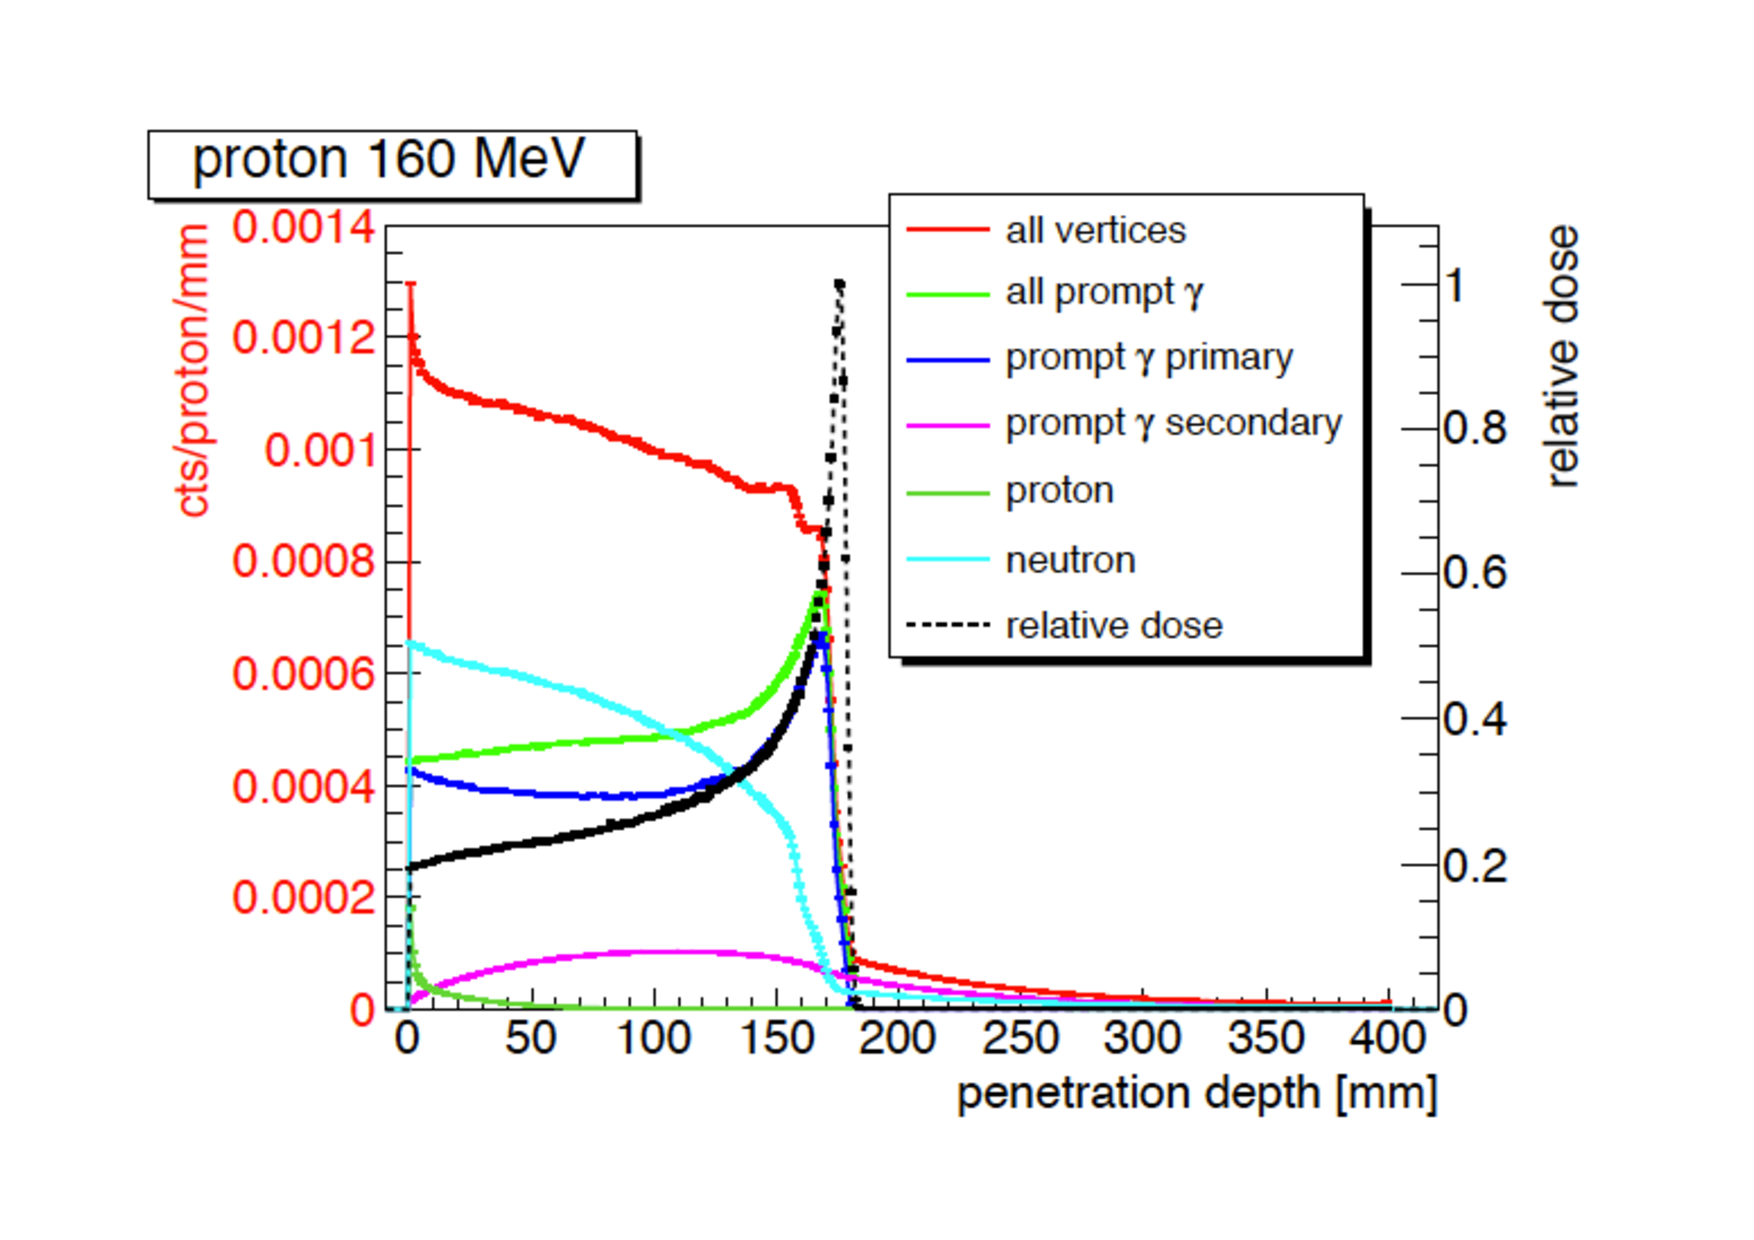
\includegraphics[width=1.3\linewidth]{03_GraphicFiles/chapter2_GammaCameras/PG_secPartDistr_p.pdf}
\caption{Emission vertices of secondary particles emerging from a cylindrical water target (15~cm diameter, 40~cm length) irradiated by a 160~MeV proton beam. An energy lower threshold of 1~MeV has been applied.}
\label{chap2::fig::PGsecDistrp}
\end{subfigure}
\begin{subfigure}[t]{.49\textwidth}
\hspace{-1cm}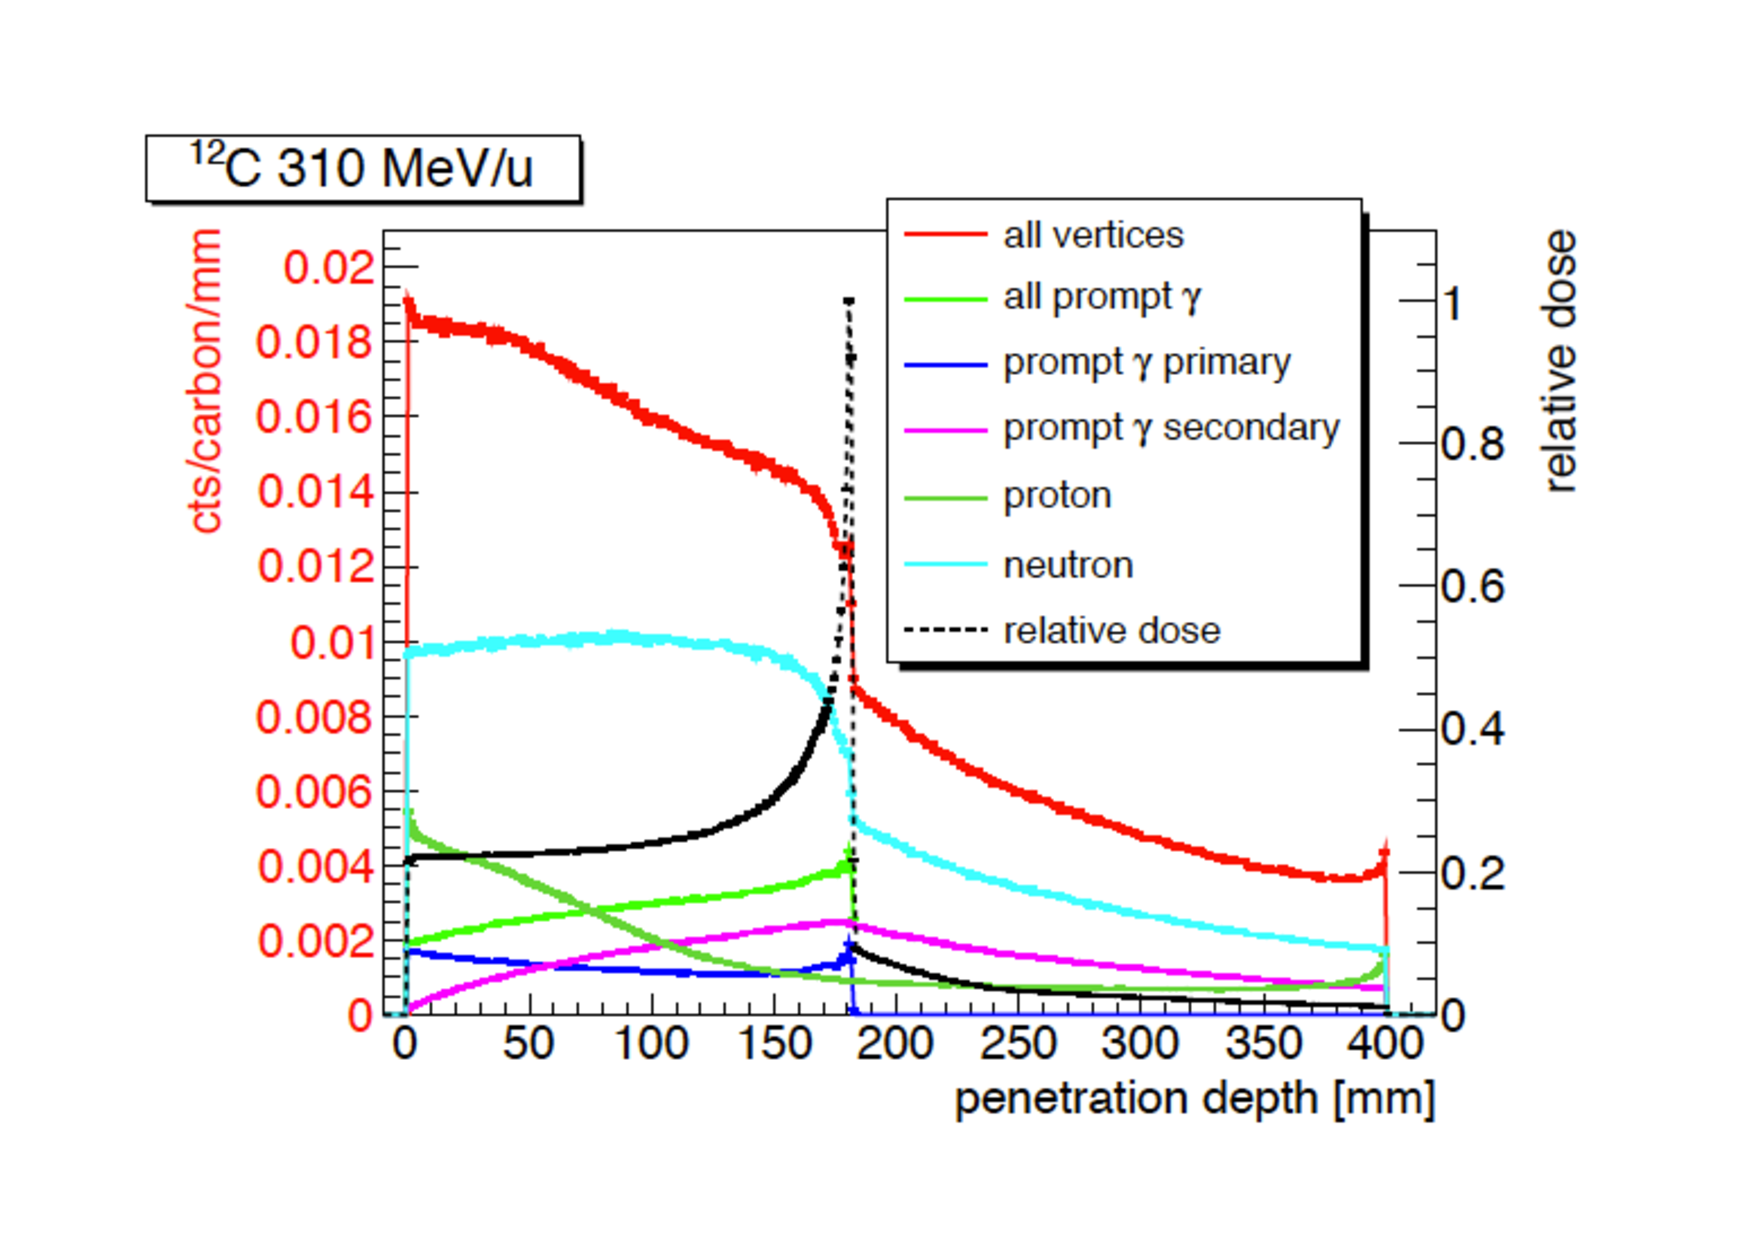
\includegraphics[width=1.3\linewidth]{03_GraphicFiles/chapter2_GammaCameras/PG_secPartDistr_C.pdf}
\caption{Emission vertices of secondary particles emerging from a cylindrical water target (15~cm diameter, 40~cm length) irradiated by a 310~MeV/u carbon ion beam. An energy lower threshold of 1~MeV has been applied.}
\label{chap2::fig::PGsecDistrC}
\end{subfigure}
\caption{In~\cite{Krimmer2017}.}
\label{chap2::fig::PGsecDistr_gen}
\end{figure}

\figurename~\ref{chap2::fig::PGsecDistr_gen} shows the distribution of emission vertices \myMarginnote{PG spatial features} of secondary radiation emitted by an homogeneous water phantom (cylinder of 15~cm diameter and 40~cm length) in the beam direction, together with the dose profile. The simulated data have been obtained by irradiating the phantom with 160~MeV protons (\figurename~\ref{chap2::fig::PGsecDistrp}) and 310~MeV/u carbon ions (\figurename~\ref{chap2::fig::PGsecDistrp}), having the same expected range in water. All the secondary particle vertex distributions are correlated to the primary ion range, and in particular \glspl{pg} appear as the best candidates for range monitoring purpose, given the significant emitted statistics. Also neutrons are produced in considerable fraction, mainly in carbon ion irradiation, but the spatial information about their production vertex is hardly retrievable.  The correlation between longitudinal \gls{pg} and dose profiles can be exploited for \enquote{imaging} monitoring approaches lo locate the Bragg peak position. Physically and electronically collimated prototypes are used to access the spatial information carried by the emitted photons, and will be described in following sections. 
In addition to the spatial information, also energy and timing \gls{pg} specific features can be used as tools to retrieve the Bragg peak position with the so-called \enquote{non-imaging techniques}. The wide energy spectrum of the produced \gls{pg} rays \myMarginnote{PG energy distribution} depends on the composition of the target material, and it is characterized by discrete lines. In \figurename{chap2::fig::PGEdistr}, the \gls{pg} energy spectrum is shown for the simulated irradiation of \gls{pe}, \gls{pmma} and water targets with a 160~MeV proton beam. The discrete spectroscopic lines are clearly visible: in particular, three lines are highlighted, corresponding to the de-excitation of $^{16}$O (6.13~MeV), $^{12}$C (4.44~MeV), and deuterium (2.22~MeV). The latter is the result of neutron capture by hydrogen, and the produced photon distribution is not correlated to the primary particle range. The comparison of the measured \gls{pg} energy spectrum to the expected one can be used to access information about the material traversed by the primary beam and estimate the proton range: such a technique is referred to as \gls{pgs}~\parencite{Verburg2014}, and will be further discussed in following sections. To be noticed that the \gls{pg} yields are not only depending on the traversed material composition, but also on the beam energy; a global enhancement is observed as the energy decreases~\parencite{Krimmer2017}.  

\begin{figure}
\centering
\begin{subfigure}[t]{.49\textwidth}
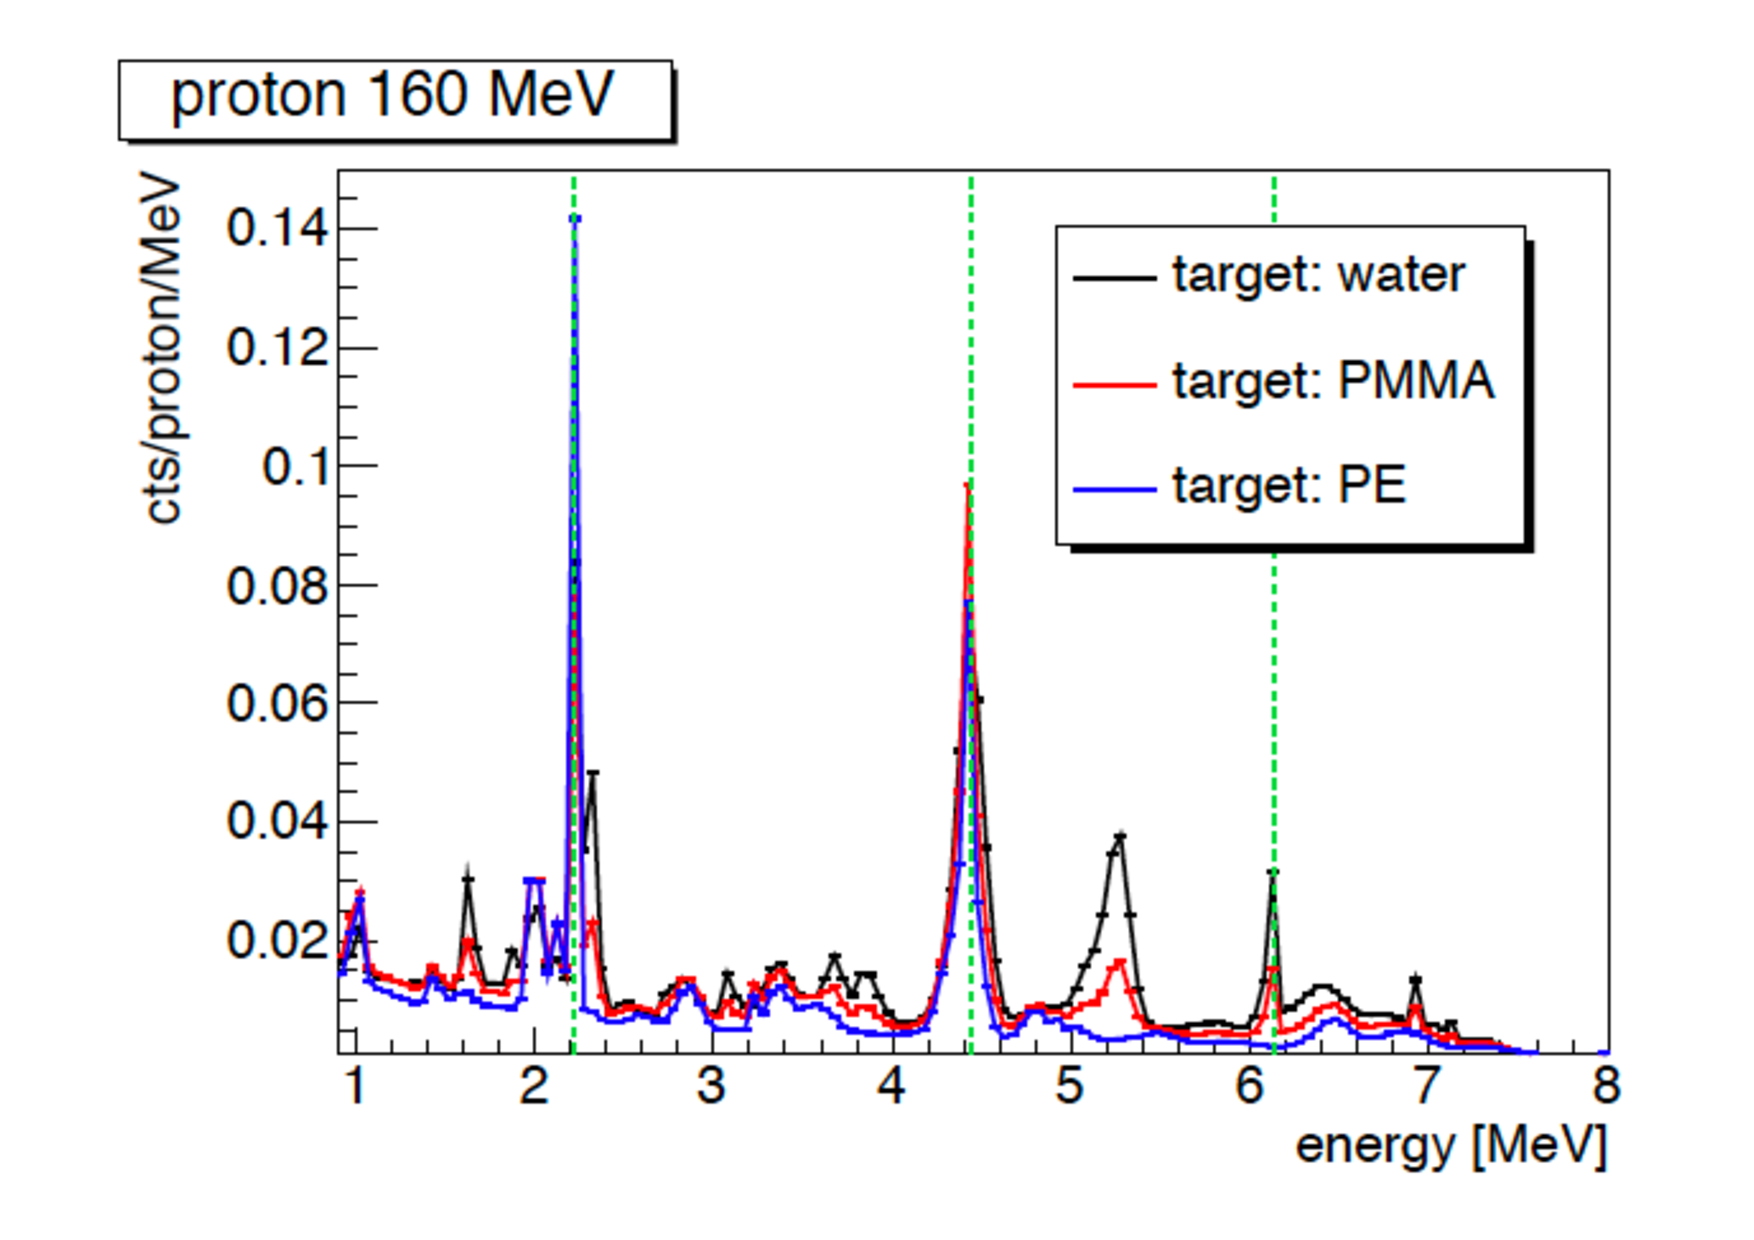
\includegraphics[width=1.\linewidth]{03_GraphicFiles/chapter2_GammaCameras/PG_E_targets.pdf}
\caption{\gls{pg} energy spectra resulting from the irradiation of \gls{pe}, \gls{pmma} and water targets (cylinders 15~cm diameter, 25~cm length) with 160~MeV protons. The vertical lines highlight specific spectroscopic transitions.}
\label{chap2::fig::PGEdistr}
\end{subfigure}
\begin{subfigure}[t]{.49\textwidth}
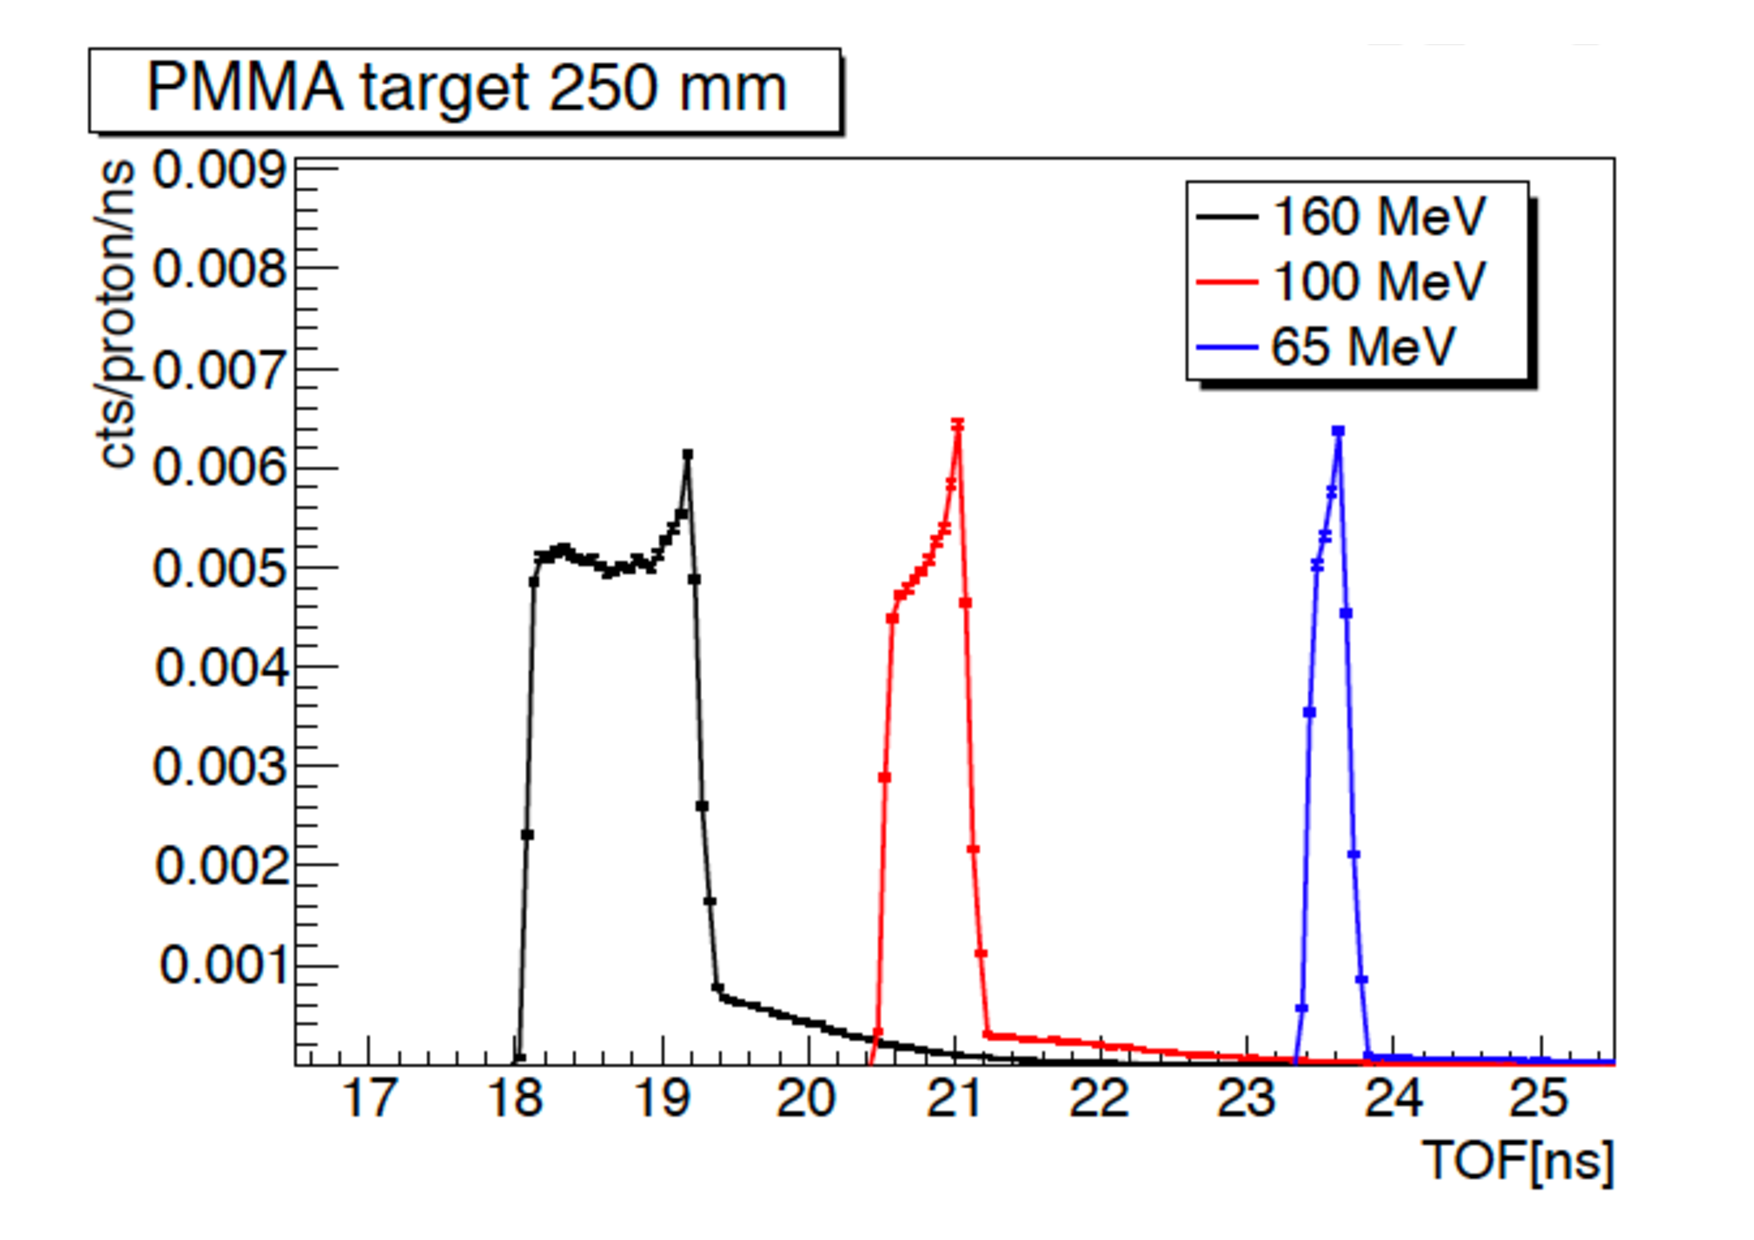
\includegraphics[width=1.\linewidth]{03_GraphicFiles/chapter2_GammaCameras/PG_TOF_PMMA.pdf}
\caption{\gls{tof} spectra of \glspl{pg} emerging from a \gls{pmma} cylindrical target (cylinders 15~cm diameter, 25~cm length) for 65~MeV, 100~MeV and 160~MeV proton beam irradiation.}
\label{chap2::fig::PGTdistr}
\end{subfigure}
\caption{In~\cite{Krimmer2017}.}
\label{chap2::fig::PG_ET}
\end{figure}

As mentioned, also time information can be used for range monitoring purpose. \myMarginnote{PG TOF distribution} \figurename~\ref{chap2::fig::PGTdistr} shows the \gls{tof} distribution of \glspl{pg} emerging from a \gls{pmma} target (15~cm diameter, 25~cm length) irradiated with 65~MeV, 100~MeV and 160~MeV proton beams. The influence of proton energy (range) on the spectrum peak position, width and integral is clear, and is the basic idea for two proposed monitoring techniques: \gls{pgt}, which is based on the \gls{tof} spectrum peak position and width~\parencite{Golnik2014}, and \gls{pgpi}, additionally exploiting the \gls{tof} spectrum integral to verify beam position and total dose, thus apporaching in vivo dosimetry~\parencite{Krimmer2017b}. 

All monitoring techniques based on \glspl{pg} must commonly deal with some specific \gls{pg} features. As a starting point, \gls{pg} production yields must be considered when designing monitoring prototypes. 
Specific measurements are needed for particle therapy, with peculiar beam energies, targets and irradiation fields, even if some data of \gls{pg} production by proton and carbon ions are available in the literature for general nuclear physics and astrophysics purposes~\parencite{Dyer1981, Kiener1998}.
In~\cite{Pinto2015} the authors studied the absolute \gls{pg} production yields in ten single-slit experiments with the irradiation of \gls{pmma} and water targets with proton and carbon ion beams, and the results are shown in \figurename~\ref{chap2::fig::PG_yields} for proton (left) and carbon ion beams (right) and summarized in table~\ref{chap2::tab::PG_yields_tab}, reproduced from the same publication. 

\begin{figure}
\centering
\begin{subfigure}[t]{.49\textwidth}
\hspace{-0.7cm}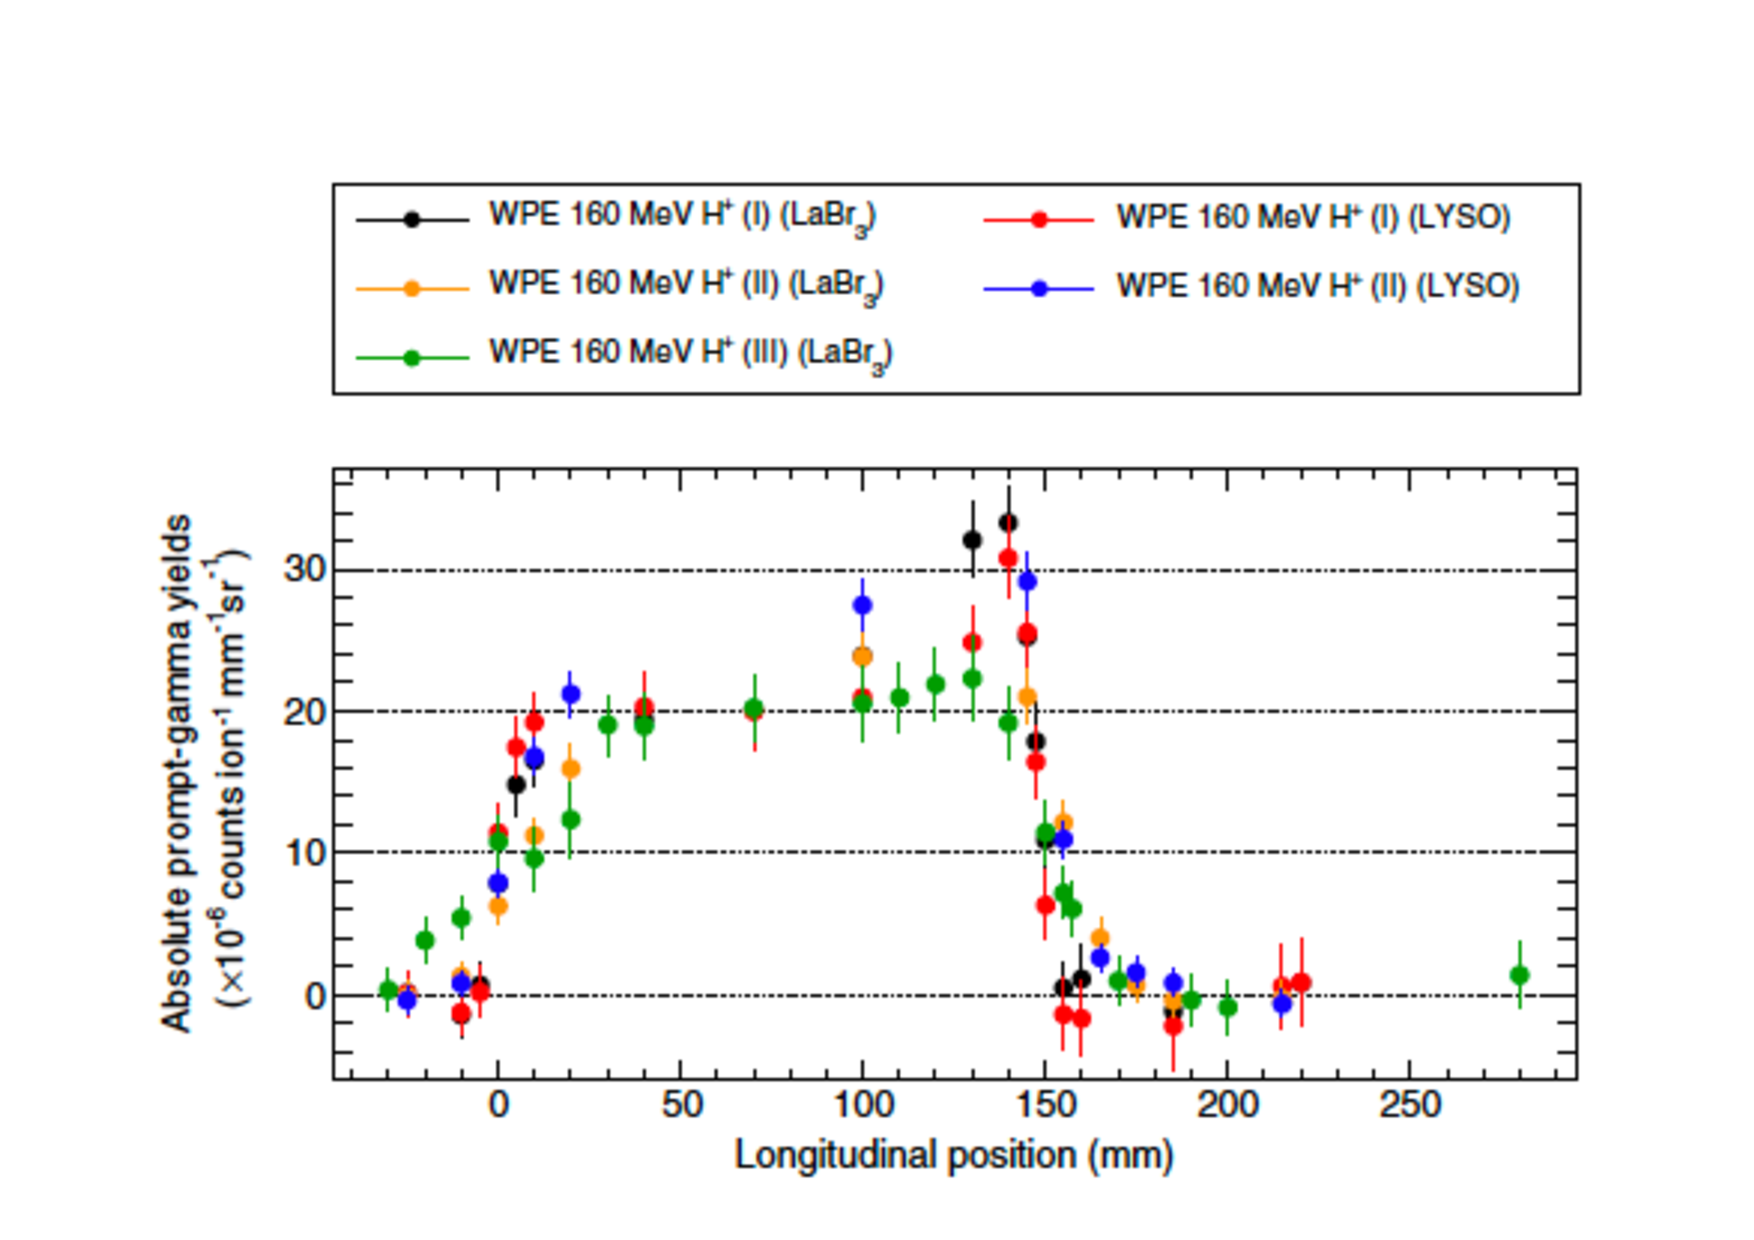
\includegraphics[width=1.2\linewidth]{03_GraphicFiles/chapter2_GammaCameras/PG_absYields_p.pdf}
\caption{Absolute \gls{pg} yields profiles for 160~MeV proton beam irradiation of a \gls{pmma} target. The different colors represent 5 different data sets, 3 obtained with \gls{labr3} detector, 2 with \gls{lyso} detector.}
\label{chap2::fig::PG_absYields_p}
\end{subfigure}
\begin{subfigure}[t]{.49\textwidth}
\hspace{-0.7cm}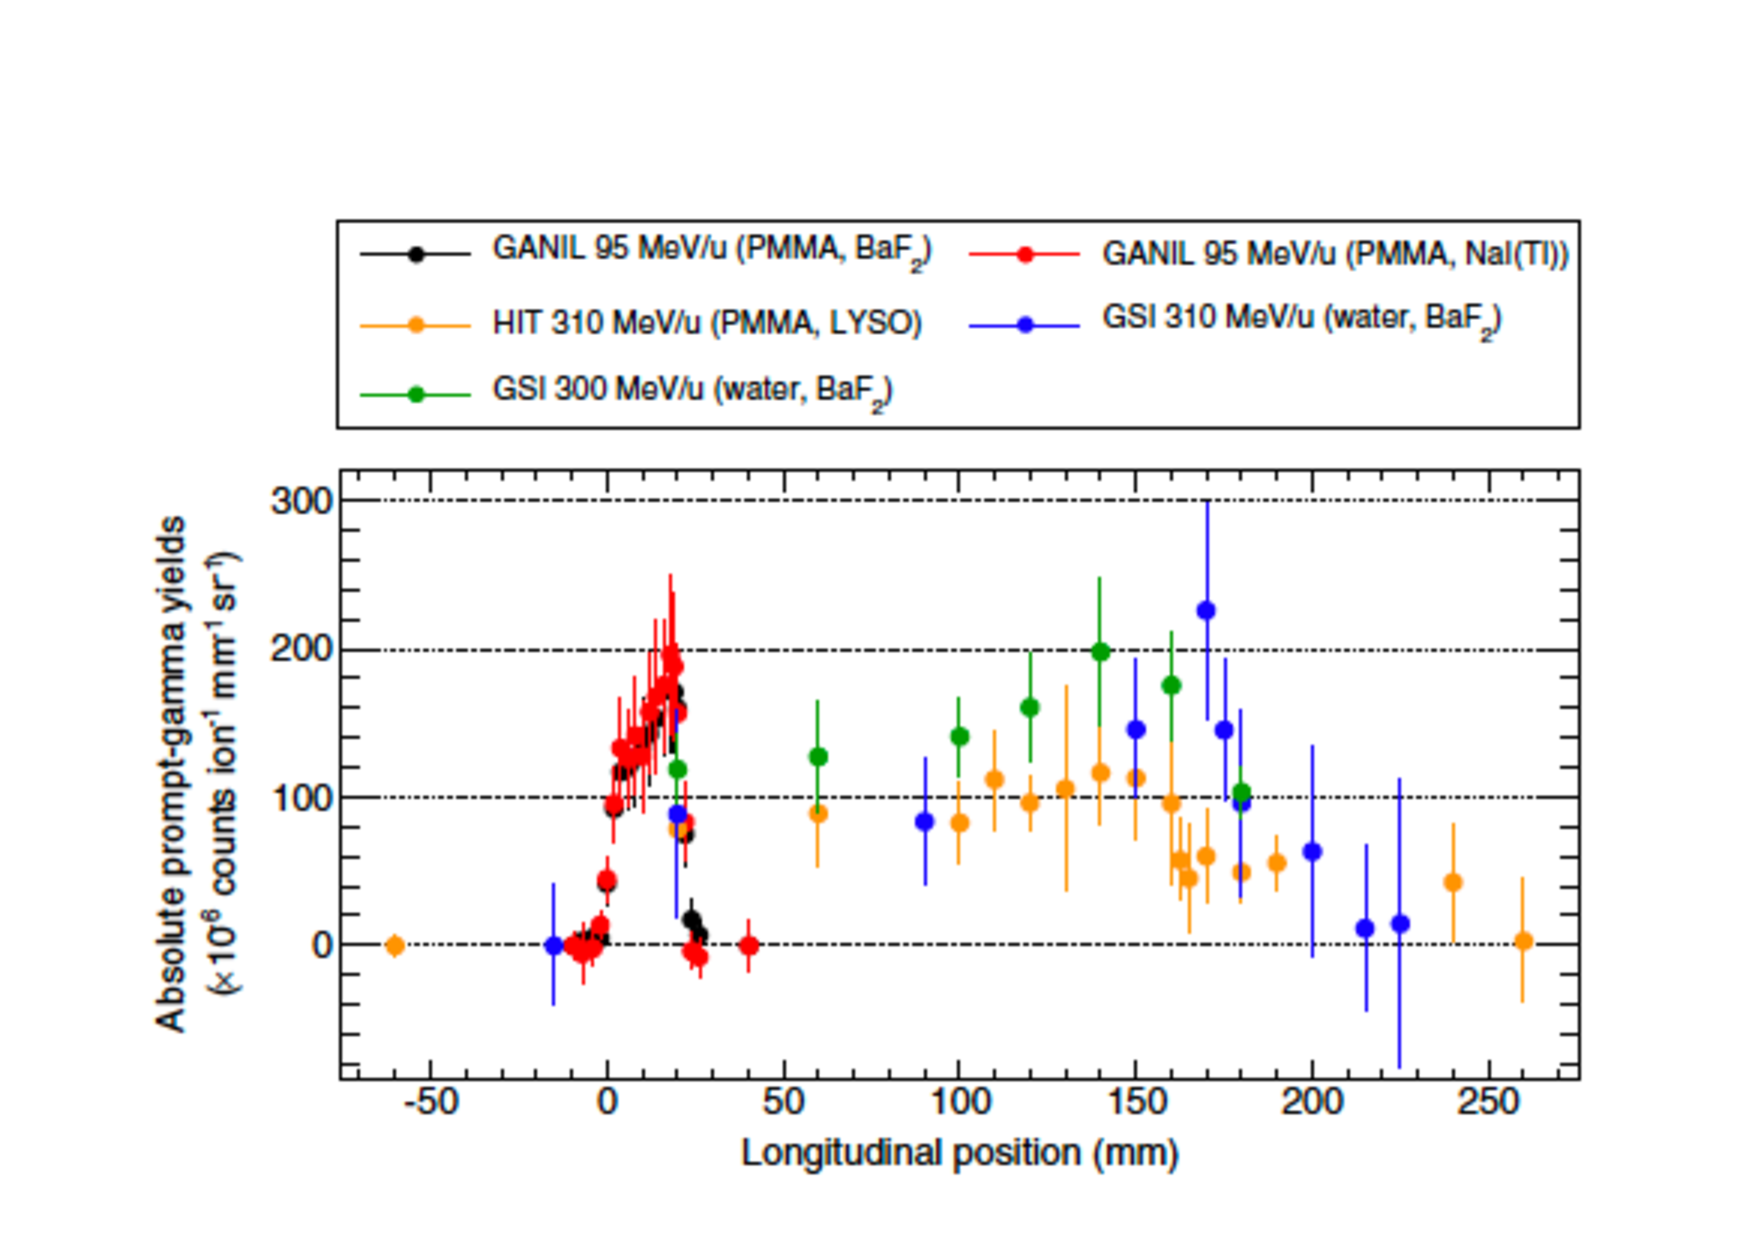
\includegraphics[width=1.2\linewidth]{03_GraphicFiles/chapter2_GammaCameras/PG_absYields_C.pdf}
\caption{Absolute \gls{pg} yields profiles for carbon ion beam irradiation of a \gls{pmma} target. The different colors represent 5 different data sets, collected at \gls{ganil}, \gls{hit} and \gls{gsi} with 95~MeV/u, 310 MeV/u adn 300~MeV/u carbon ion beams respectively. \gls{pmma} and water targets have been employed, and the \gls{pg} detection has been performed with \gls{baf2}, \gls{lyso} and gls{naitl} detectors.}
\label{chap2::fig::PG_absYields_C}
\end{subfigure}
\caption{In~\cite{Pinto2015}.}
\label{chap2::fig::PG_yields}
\end{figure}

\begin{table}[!htbp]
\centering
\caption{Absolute \gls{pg} yields measured in the first point after the \gls{pg} profile entrance rise. The energy range shows the energy range of the primary particles inside the \gls{fov} of the measurement point estimated in simulation. Table reproduced from~\cite{Pinto2015}.}
\label{chap2::tab::PG_yields_tab}
\resizebox{\textwidth}{!}{%
\begin{tabular}{llcc}
\toprule
\rowcolor{myColorMainA!20} 
\textbf{Material}& \textbf{Energy range (MeV/u)} & \textbf{Ion species} & \textbf{Absolute yield [$\times$10$^{-6}$ counts ion$^{-1}$mm$^{-1}$sr$^{-1}$]} \\
\midrule
\gls{pmma} & [77-90] & Carbon ions & 124 $\varpm$ 0.7 $_{\mathrm{stat}} \varpm$ 30 $_{\mathrm{sys}}$\\
\gls{pmma} & [272-310] & Carbon ions & 79 $\varpm$ 2 $_{\mathrm{stat}} \varpm$ 23 $_{\mathrm{sys}}$\\
Water          & [264-292] & Carbon ions & 112 $\varpm$ 1 $_{\mathrm{stat}} \varpm$ 22 $_{\mathrm{sys}}$\\
\gls{pmma} & [139-156] & Protons & 16 $\varpm$ 0.07 $_{\mathrm{stat}} \varpm$ 1 $_{\mathrm{sys}}$\\
\bottomrule
\end{tabular}}
\end{table}    

The comparison of \gls{pg} yields for proton and carbon ion beam irradiation with the same range in water, i.e. 160~MeV protons and 310~MeV/u carbon ions, shows a value approximately five times greater for the latter with respect to the former. Such an increased emission is due to the contribution of both projectile and target nuclei, while only the target nuclei can emit \glspl{pg} in proton irradiation. For carbon ions irradiation at different energies, an increased \gls{pg} emission has been verified for the lowest energy ions, as expected from published cross sections. Moreover, if comparing the \gls{pmma} and water targets for the same primary ion features, water results in an enhanced prompt photon emission. 
Other experimental results are reported in~\cite{Agodi2012, Agodi2013}: the authors measured \gls{pg} yields of 80~MeV/u carbon ions impinging on a \gls{pmma} target considering the full ion range, while in~\cite{Pinto2015} the results are normalized to the path length unit (1~mm). The found yield is (2.32$\varpm$0.01$_{\mathrm{stat}} \varpm$ 0.15 $_{\mathrm{sys}}$) $\times$ 10$^{-3}$ counts ion$^{-1}$sr$^{-1}$, which is compatible to the results in~\cite{Pinto2015} if the proper normalization is considered. Higher energy carbon ion beams (220~MeV/u) and \gls{pmma} targets have been employed to produce the results presented in~\cite{Mattei2015}. More recently, the same authors studied the prompt photon production of $^{4}$He, $^{12}$C and $^{16}$O beams interacting in \gls{pmma} target at \gls{hit}, showing good agreements with the aformentioned results (for carbon ions), and providing additional information about new ion species~\parencite{Mattei2017}. 
Furthermore, detailed information about specific \gls{pg} spectroscopic lines are reported in~\cite{Verburg2014, Verburg2013}, and have been recently published in~\cite{Kelleter2017}.

In order to resume the present knowledge about \gls{pg} production and give reference values for clinical applications, as reported in~\cite{Krimmer2017}, a rough estimate of the \gls{pg} yields per projectile for 15~cm range in water is 0.05 per proton and about 0.3 per carbon ion. These yields results to be similar to the one of the total amount of $\beta^{+}$ emitters~\parencite{Pinto2015, Robert2013}. However, Secondary radiation attenuation is another fundamental parameter to be considered, since only a fraction of the emitted photons will be able to emerge from the patient body and, at the same time, keep the information on the creation vertex. The higher energies of prompt photons (1-10~MeV) with respect to positron annihilation ones (511~keV) lead to an improved transmission through the patient body (factor 5), thus an increased expected detection rate~\parencite{Moteabbed2011}. 
The available \gls{pg} statistics for beam range monitoring can be assessed by considering the absolute yields measurements presented above (including attenuation considerations) and the average clinical beam intensities. In particular, 10$^{10}$ protons per second and 10$^{[7-8]}$ carbon ions per second are typical clinical values. For a monitoring on a single spot basis, which is highly desirable, the most important spot (generally in the distal region of the \gls{ptv}) can be chosen as reference: the number of incident ions in such a spot is approximately 10$^8$ and $10^6$ for protons and carbon ions, respectively~\parencite{Kramer2000, Grevillot2012}. For these kinds of spots, in the whole solid angle, about 10$^7$ (for protons) and 10$^5$ (for carbon ions) \gls{pg} rays are emitted in the spot duration. This number is then reduced by the detection device efficiency and \gls{fov}. 

\subsubsection{Simulation of prompt-gamma emission and detection}\label{chap2::subsec::PGsimulation}

The general objective of \gls{pg} control of particle therapy treatment is the ion range on-line monitoring, which is performed via a comparison between measured and predicted \gls{pg} distributions, in accordance with the treatment planning. The prediction of \gls{pg} emission profiles relies on simulations, which are based on the experimental data described in the previous paragraph, and must include the prediction of the detector response. Precision and accuracy of the physical models and the reference data are crucial in the simulation process, also given the complex dependency of \gls{pg} yields to parameters such as beam features (ion species, energy, spatial distribution) and target composition. 

Monte Carlo simulation approaches are generally time consuming~\parencite{Robert2013, Dedes2015, Schumann2015}, and several approaches are being studied to reduce the calculation time and allow for direct translation to clinics. \gls{gpu}-oriented implementations highly improves the simulation efficiency, and some solutions have been successfully tested. Clinically acceptable dose calculation accuracy has been achieved with few tens of seconds of calculation time required, but electron and neutron transport have been disabled in the code described in~\cite{Qin2017}. With respect to standard Monte Carlo codes, an improvement in efficiency of three orders of magnitude is reported for the clinical validation of the code gPMC (\gls{gpu}-based \gls{mc} code for proton dose calculation ) in~\cite{Giantsoudi2015}. 
Alternative approximate methods are based on the \gls{vrt}, already implemented, for example, for in-beam \gls{pet} predictions~\parencite{Sommerer2009}. It has been shown that computation time can be reduced by about three orders of magnitude for the prediction of full three-dimensional \gls{pg} maps with respect to standard \gls{mc} codes~\parencite{Huisman2016, ElKanawati2015}. The calculation can be achieved in about two hours on a single core computer; this makes the clinical implementation possible, even if further improvements are still needed.  
As a general remark, it must be noticed that \gls{mc} tool-kits have not been conceived for the energy range of interest in particle therapy, thus a fine tuning of the model parameters is necessary. The comparison of different \gls{mc} codes often results in large differences in the \gls{pg} simulated yields~\parencite{Bohlen2010, Verburg2012, Schumann2015}, and the hadronic models still have to be improved, ideally with the availability of differential cross-sections and \gls{pg} yields further measurements in the clinical energy range~\parencite{Newhauser2015}. However, substantial enhancement have been achieved in the \gls{qmd} model~\parencite{Dedes2014}, and quantitative characterization of \gls{pg} emission yields have been performed~\parencite{Schumann2015, Pinto2016}.

In addition to \gls{mc}-based approaches, also the implementation of analytic models is efficient~\parencite{Sterpin2015, Russo2016}, even if they are based on pre-computed \gls{pg} profiles obtained with \gls{mc} calculations, thus they suffer from the aforementioned uncertainties.
Finally, the pre-computation of \gls{pg} profiles is not required by filtering approaches, which make use of the dose distribution maps, available form the treatment planning, and directly get the expected \gls{pg} distribution~\parencite{Kroniger2015}.  
  
\subsection{PG ion range monitoring devices: state of the art}\label{chap2::sec::PGdevices}

The detection of \gls{pg} rays for particle therapy monitoring has been proposed already in 2003~\parencite{Stichelbaut2003}, and since then several approaches have been investigated by developing adapted detection devices. The specificity of particle therapy range control techniques based on \glspl{pg} requires the design of dedicated detectors, adapted to a wide photon energy spectrum and able to cope with the background level expected during particle therapy treatments. Standard medical imaging cameras, like the Anger cameras employed for \gls{spect} examinations, cannot be adapted to such requirements. 
The explored solutions to create clinical prototypes can be classified, as proposed in~\cite{Krimmer2017} and already mentioned in this chapter, in imaging devices, based on the spatial information provided by each collected prompt photon, and non-imaging ones, which exploit integrated prompt photon yields. In table~\ref{chap2::tab::PGmodalities_tab}, reproduced from~\cite{Krimmer2017}, the main features exploited by the developed modalities are summarized.

\begin{table}[!htbp]
\centering
\caption{Characteristics of the \gls{pg} monitoring modalities. The star symbol represents mandatory measurements, the star in brackets means auxiliary but not mandatory measurements. Table reproduced from~\cite{Krimmer2017}.}
\label{chap2::tab::PGmodalities_tab}
\resizebox{\textwidth}{!}{%
\begin{tabular}{l | ccccc}
\toprule
\rowcolor{myColorMainA!20} 
\textbf{PG} & \multicolumn{2}{c}{\textbf{Imaging systems}} & \multicolumn{3}{c}{\textbf{Non-imaging systems}} \\ 
%\rowcolor{myColorMainA!20} 
%\cmidrule(lr){2-3}\cmidrule(lr){4-6}
\rowcolor{myColorMainA!20} 
 \textbf{features}   & Physical & Electronic & PG timing & PG peak integral & PG spectroscpy\\
\rowcolor{myColorMainA!20} 
    & collimation & collimation & (PGT) & (PGPI) & (PGS)\\    
\midrule
Position & $\star$ & $\star$&  & &  \\
Energy & ($\star$) & ($\star$) & ($\star$) &  ($\star$) & $\star$\\
TOF & ($\star$) & ($\star$) & $\star$& $\star$& ($\star$) \\
\bottomrule
\end{tabular}}
\end{table}      

In the following sections, the state of the art of the various \gls{pg} monitoring modalities is present following the proposed classification.

\subsubsection{Non-imaging prototypes}\label{chap2::subsec::PGdevices_nonImaging}

Non-imaging \gls{pg} monitoring solutions are based on the integrated measurement of time or energy resolved photon spectra, and exploit the indirect relation between the characteristics of such spectra and the primary ion range to verify the conformity of the delivered treatment to the planned one. The objective of such techniques is not to retrieve spatial information from the collected photons, thus less demanding detectors are required with respect to imaging solutions, and the footprint in the treatment room is minimized, as well as the device cost. 

As the primary ion beams interacting in the patient during treatments \myMarginnote{PGT} cause nuclear excitation and, thus, the emission of prompt photons along their path, until they are stopped, the total transit time depends on the total ion range. The width of the \gls{pg}-\gls{tof} spectrum can be then correlated to the ion range. Such a monitoring method has been first proposed in 2014 by Golnik and colleagues~\parencite{Golnik2014} and tested with 150~MeV protons at the AGOR cyclotron, KVI-CART. The proton beam irradiated a homogeneous graphite target (10$\times$10$\times$30~cm$^3$, density 1.7~g~cm$^{-3}$), with an expected range of 10.3~cm; the target has been set in three different positions (20~mm between each position), and the gamma detection has been performed with a \gls{gaggce} cylindrical detector.  The setup is shown on the left side of \figurename~\ref{chap2::fig::PGT_shifts}, and the resulting spectra are shown  on the right side.

\begin{figure}[!htbp]
\centering
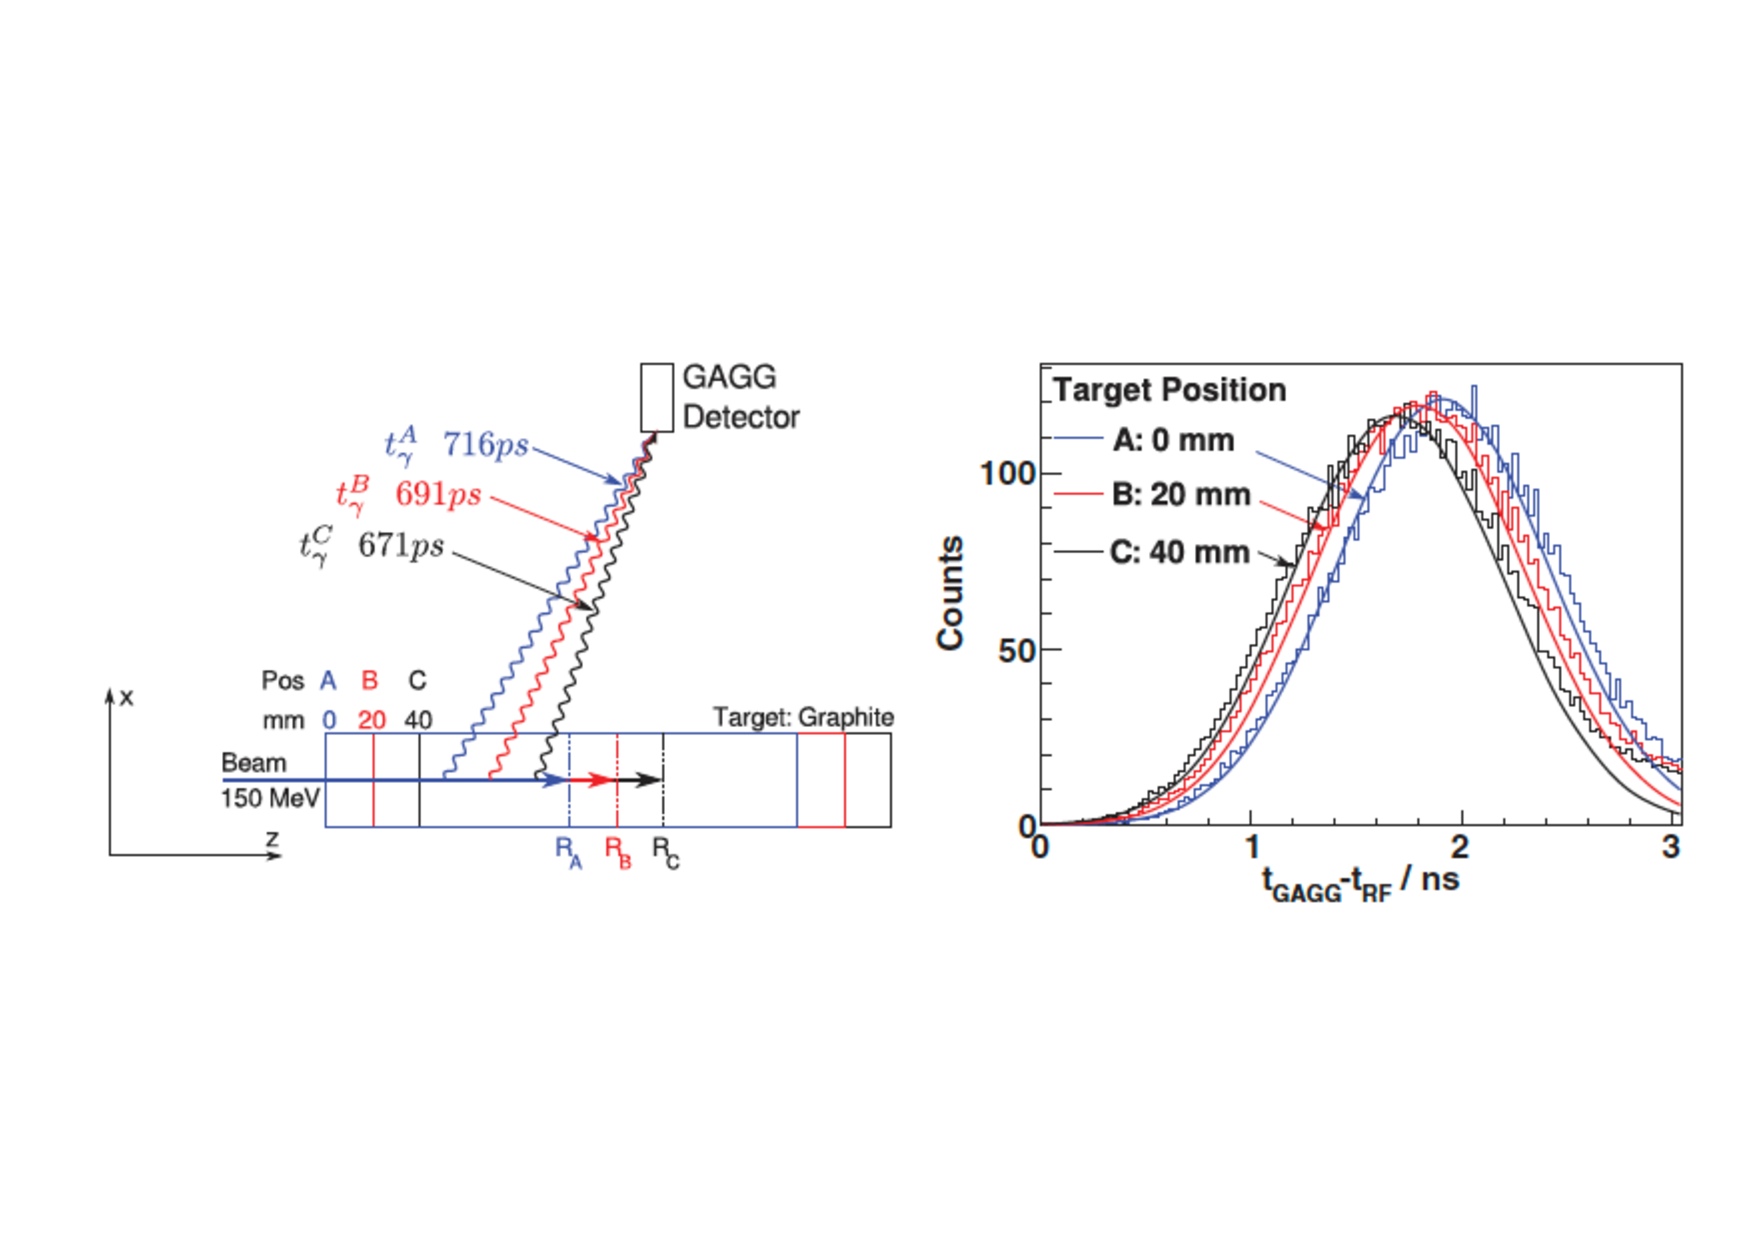
\includegraphics[width=0.9\textwidth, trim = {1cm 5cm 1cm 5cm}, clip]{03_GraphicFiles/chapter2_GammaCameras/PGT_shifts.pdf}
\caption{(Left) Setup for the irradiation of a graphite target with 150~MeV proton beams. The target was set in three different positions, with successive 20~mm shifts. (RIght) Resulting \gls{pg}-\gls{tof} spectra; the photon measurements has been performed with a \gls{gaggce} cylindrical detector. The experimental data are normalized to 10$^9$ incident protons. In~\cite{Golnik2014}.}
\label{chap2::fig::PGT_shifts}
\end{figure}  

The shift of the average spectrum position, corresponding to the target shift, is clearly visible.In the same work, the authors also present the results of the irradiation with the same proton beam (150~MeV) of \gls{pmma} target at increasing thickness, from 5 to 15~cm. The detection has been performed with the same \gls{gaggce} detector. The resulting \gls{tof} spectra are shown in \figurename~\ref{chap2::fig::PGT_PMMA}.

\begin{figure}[!htbp]
\centering
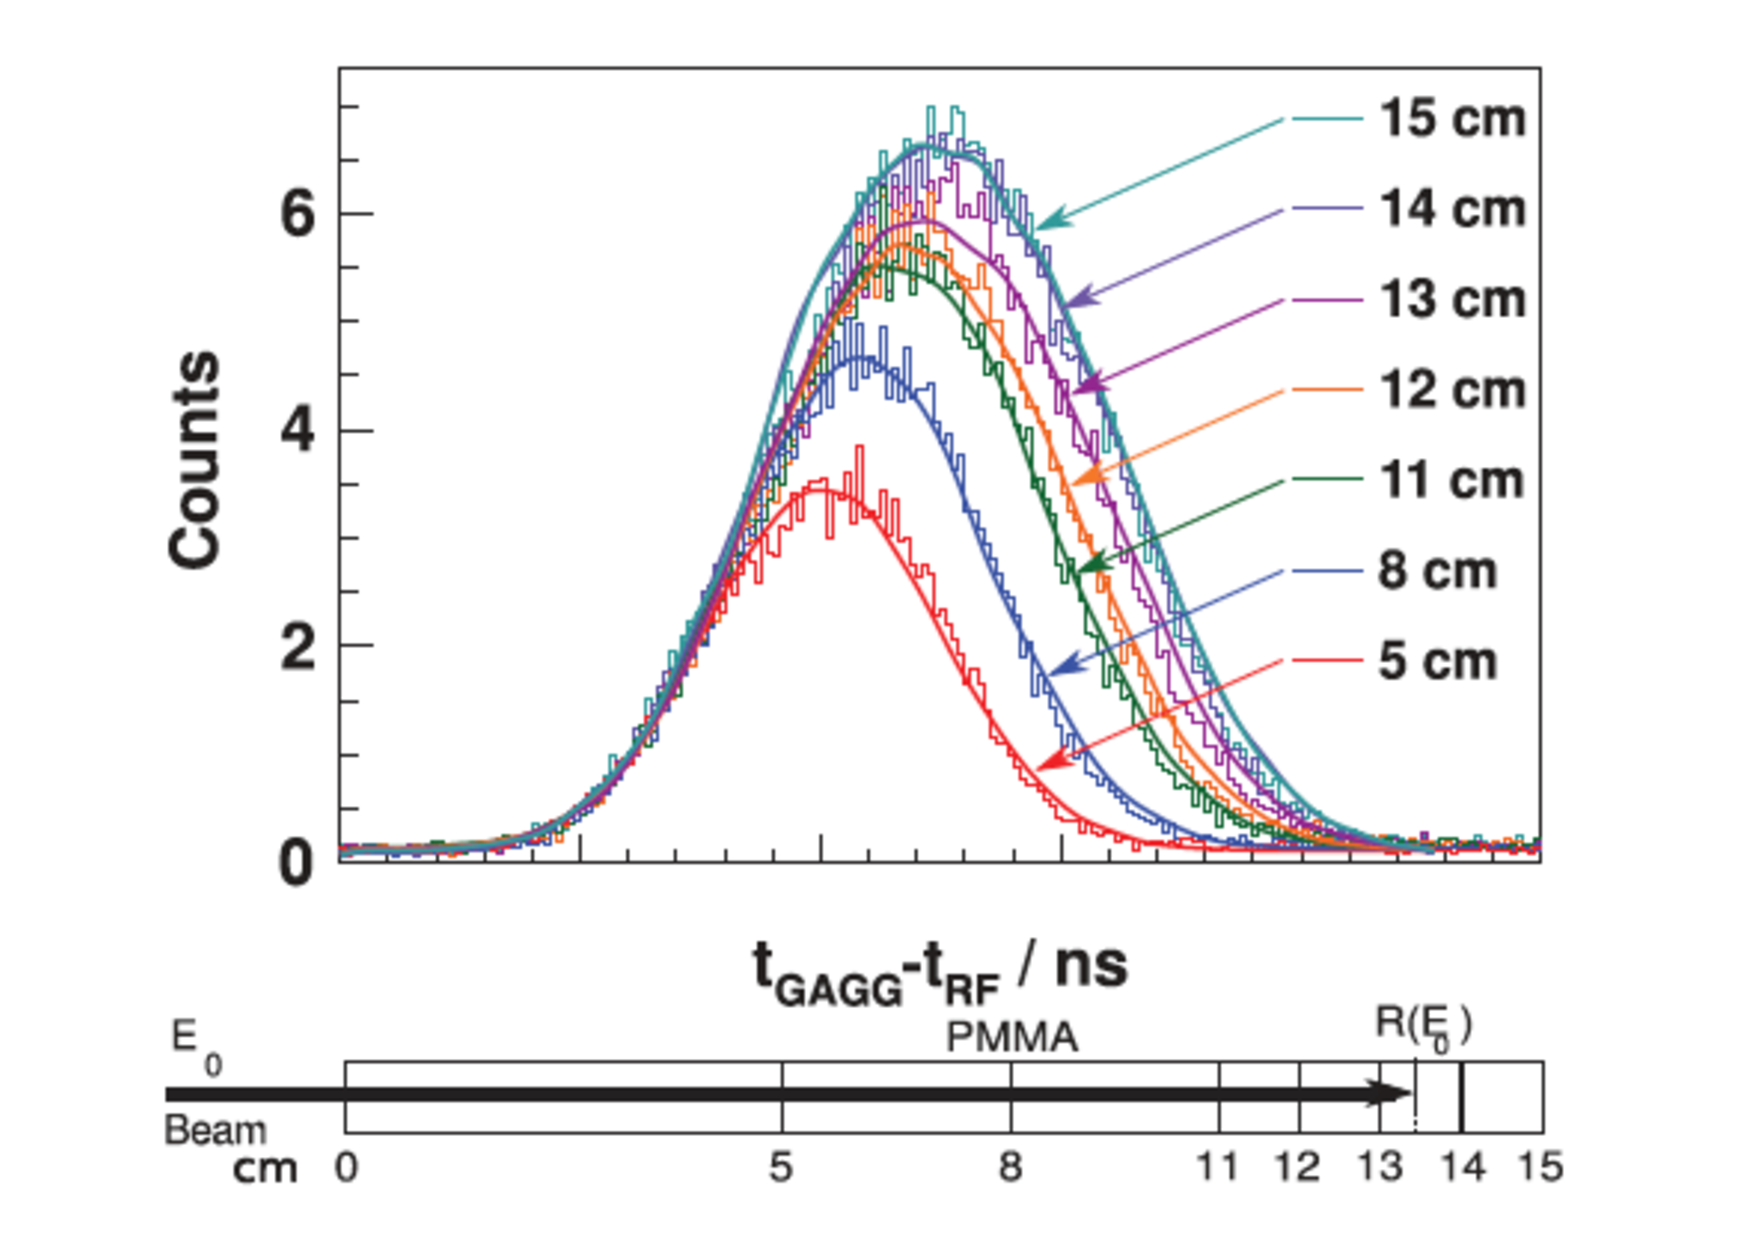
\includegraphics[width=0.8\textwidth]{03_GraphicFiles/chapter2_GammaCameras/PGT_PMMA.pdf}
\caption{Comparison of simulated and experimental \gls{pg}-\gls{tof} profiles obtained with the irradiation of \gls{pmma} targets with increasing thickness. The \gls{pg} detection is performed with a \gls{gaggce} detector. In~\cite{Golnik2014}.}
\label{chap2::fig::PGT_PMMA}
\end{figure}  

The beam expected range was 13.6~cm, so that it stopped in the target only for 14 and 15~cm thick \gls{pmma} blocks. \figurename~\ref{chap2::fig::PGT_PMMA} shows the good agreement between simulated (solid lines) and experimental data (histograms), and the shift and broadening of the \gls{pg}-\gls{tof} spectra with the increasing target thickness. Similar results have been also obtained by simulating proton beams at increasing energies, from 50 to 230~MeV, corresponding to a range change in the range [2-17]~cm. Simulation studies also included the irradiation of heterogeneous targets, and the experimental clinical verification was performed at the proton treatment center in Essen, equipped with an \gls{iba} C230 cyclotron, with several phantoms and detectors. The range variations in a stacked \gls{pmma} target, as well as the effect of air cavities and bone inserts have been verified, and the \gls{pgt}-based range verification showed the ability to detect 5~mm range shifts in heterogeneous targets for clinical relevant doses, but the strong influence of the accelerator \gls{rf} signal stability has also been highlighted~\parencite{HuesoGonzalez2015b}. The \gls{tof} measurement was actually based on the accelerator \gls{rf} signal, and a phase variation on the time-scale of hours caused shifts in the \gls{tof} spectrum equivalent to the one provoked by the shift of the target of a few centimeters. The author pointed out the need of a beam monitoring system to provide the time reference for the \gls{tof} measurement; such a beam monitor has been developed and tested to characterize the bunch structure of the clinical C230 cyclotron of the Oncoray center in Dresden~\parencite{Petzoldt2016}. 
In \figurename~\ref{chap2::fig::PGT_stats} the authors show the ability of this monitoring method to detect range shifts due to target in-homogeneity for decreasing amount of primary protons: shifts due to bone and air inserts in an homogeneous \gls{pmma} can be detected for primary statistics down to 10$^8$ primary protons, with increasing uncertainty for decreasing number of primaries.  

\begin{figure}[!htbp]
\centering
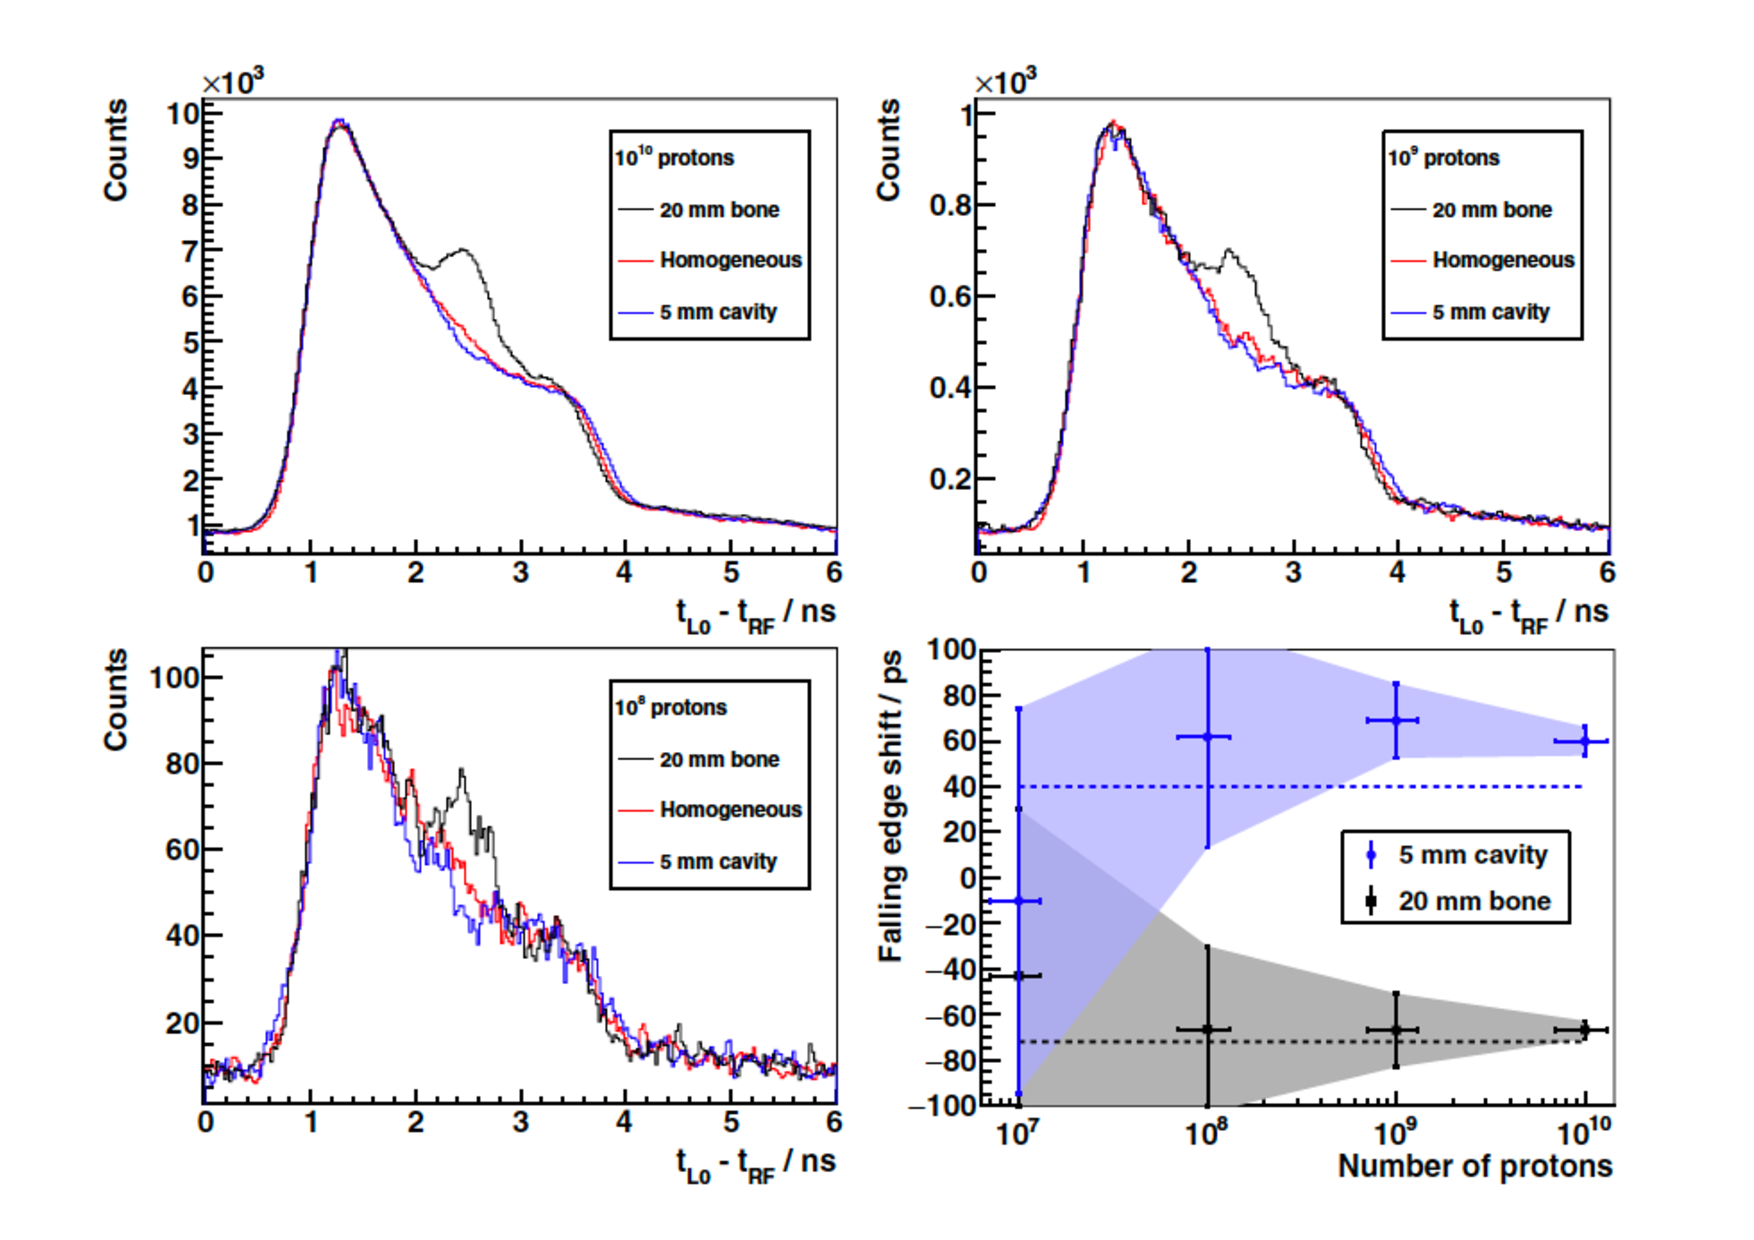
\includegraphics[width=0.9\textwidth]{03_GraphicFiles/chapter2_GammaCameras/PGT_stats.pdf}
\caption{First three panels: \gls{pg}\gls{tof} spectra obtained with the 230~MeV proton irradiation of an homogeneous \gls{pmma} target and two targets with air and bone inserts are compared for increasing number of primary protons. The \gls{pg} detection is performed with an \gls{labr3} detector (L0). The bottom right panel shows the shift of the spectra falling edge with respect to the homogeneous target case as a function of the number of incident protons. In~\cite{HuesoGonzalez2015b}.}
\label{chap2::fig::PGT_stats}
\end{figure}  

It has been estimated in~\cite{Pausch2016} that 10$^4$ detected \gls{pg} rays are needed to reveal a 5~mm range shift, with a bunch width of 2~ns.This is a fundamental requirement to be taken into account when designing a prototype for this application, together with the expected data throughput, which is significant given the absence of collimation system. However, with energy selected gamma rays of several MeV, a timing resolution of 200~ps have been obtained with optimized detector configurations (\gls{cebr3} scintillators coupled to compact U100 energy and timing spectrometer specifically developed for this application), and throughput rates of about 600 kcps (kilo counts per second) have been handled~\cite{Pausch2016}. 

The time resolved measurement of \gls{pg} rays\myMarginnote{PGPI} is also exploited in the \gls{pgpi} monitoring method. The integral of the \gls{pg} peak in the \gls{tof} spectrum measured with various detectors located at different positions around the target is used to control the ion range. After preliminary studies at the in Arronax cyclotron in Nantes, experimental tests have been performed at the \gls{cal} in Nice, following previous results published in~\cite{Carnicer2012} and obtained with the same accelerator. 65~MeV protons at an intensity of 3$\times$10$^9$ protons per second have been used to irradiate an homogeneous \gls{pmma} target, and the \gls{pg} rays have been collected with \gls{labr3} scintillators read-out with a dedicated card developed at the \gls{ipnl}. The accelerator \gls{rf} signal or a beam monitoring system have to be used to provide the time reference for the \gls{tof} measurement. For this first study, the data have been synchronized to the positions of the modulator wheel used for passive beam delivery, provided via a photosensor. In \figurename~\ref{chap2::fig::PGPI_spectra} the \gls{pg} spectra collected for two different positions of the modulator (corresponding to the maximum thickness and the hole) are shown~\parencite{Krimmer2017b}. The integral is calculated after background subtraction and the selection of the \gls{tof} proper window for the \gls{pg} selection, and compared for different detectors in various positions. The ratios of the integrals measured in different positions are able to show few percent variations in the \gls{pg} emission rate, corresponding to few millimeter range deviations, with simple and quick analytic data processing.

\begin{figure}[!htbp]
\centering
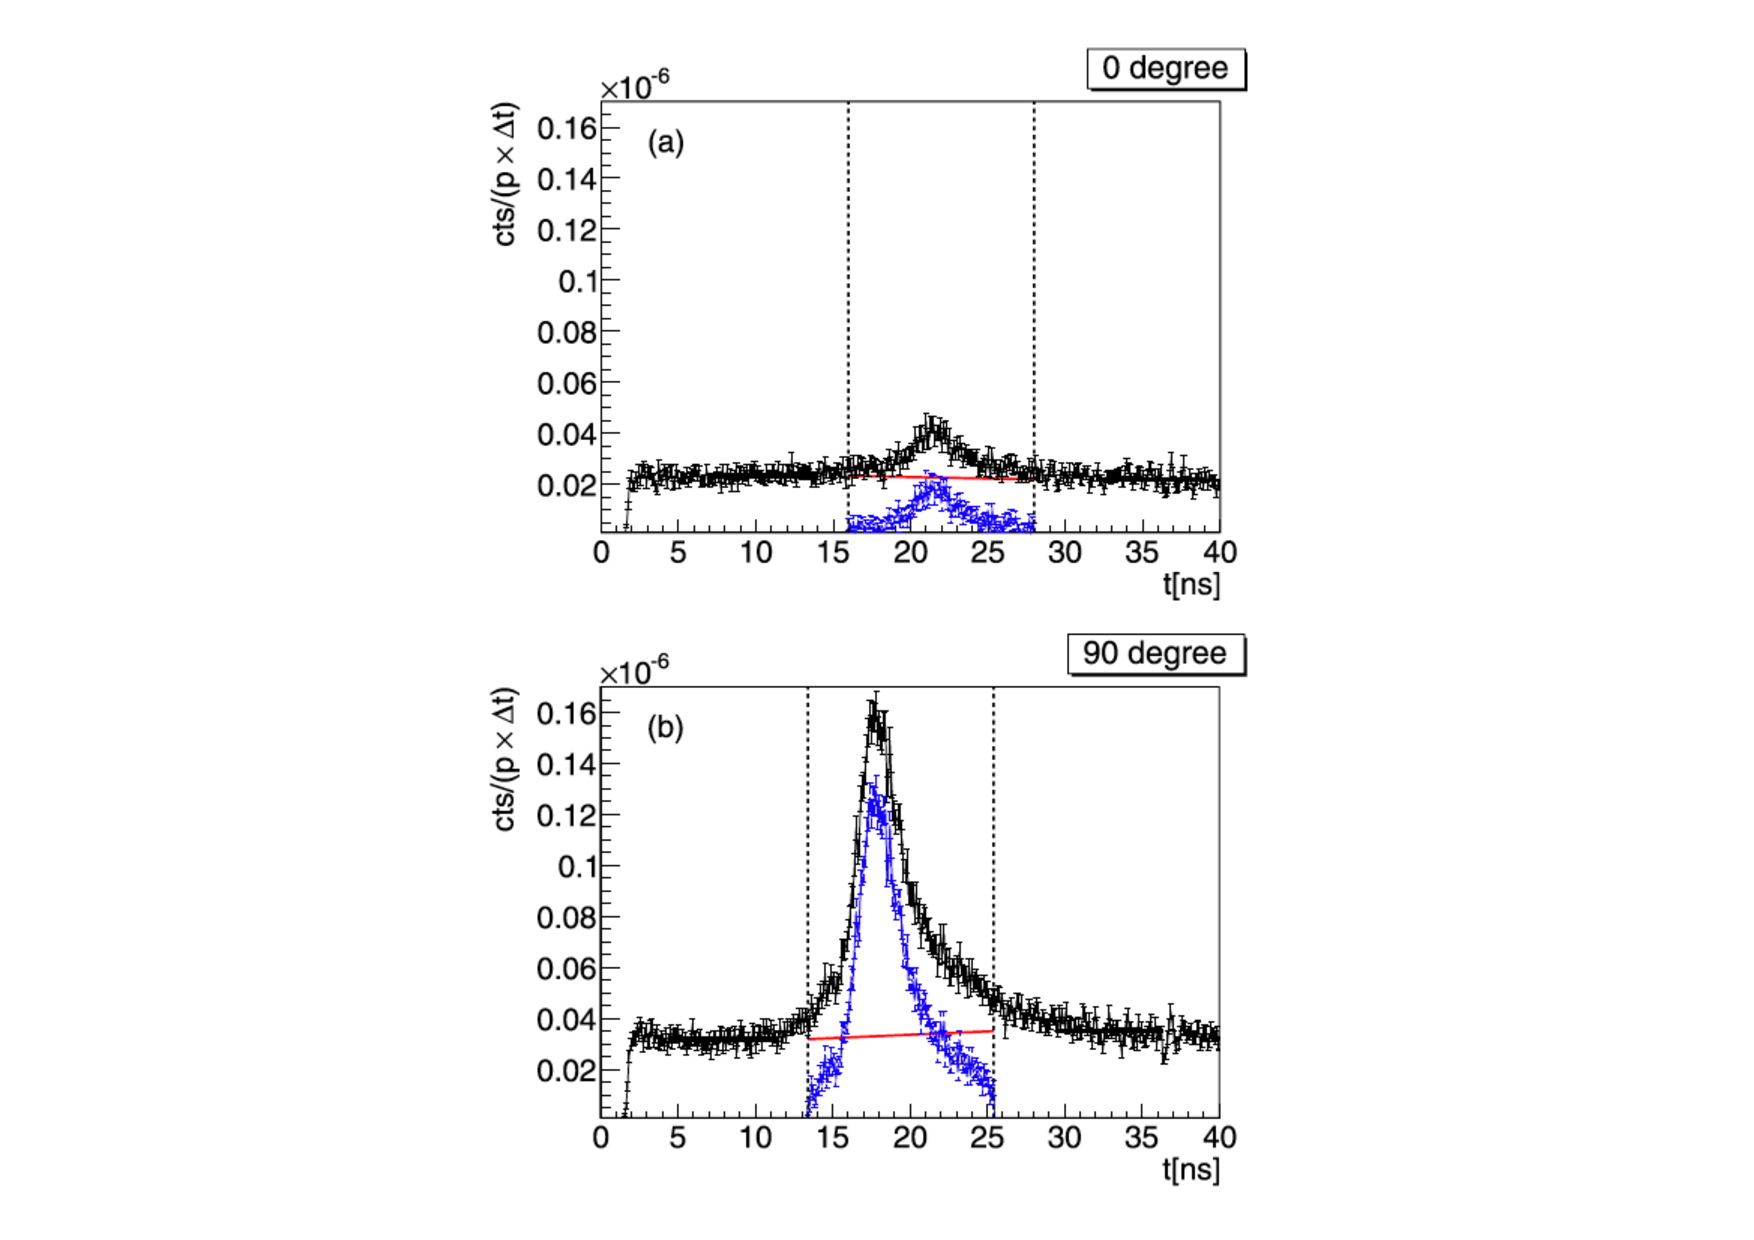
\includegraphics[width=0.9\textwidth]{03_GraphicFiles/chapter2_GammaCameras/PGPI_spectra.pdf}
\caption{\gls{tof} spectra measured for two positions of the modulator wheel, corresponding to the maximum thickness (0\textdegree) amd the hole (90\textdegree). An energy threshold of 1~MeV have been applied for the gamma detection. After background subtraction (red line), the integral is calculated in the range delimited by the vertical dashed lines. In~\cite{Krimmer2017}.}
\label{chap2::fig::PGPI_spectra}
\end{figure}  

In the case of 65~MeV protons, such a method has been verified to be able to detect 3~mm range shifts in \gls{pmma}. In addition, the authors also highlight that absorption in the target can determine similar effects on the \gls{pg} spectra, so that with the combination of signals from several detectors placed around the target, its position can be retrieved~\parencite{Krimmer2017b}.

As an alternative to time-resolved measurements\myMarginnote{PGS}, spectroscopic \gls{pg} analysis can provide indirect information about the ion range in matter through the direct estimate of the target composition. Initial studies Further studies on the \gls{pg} energy spectra have been performed in simulation and with experimental measurements with germanium detectors~\parencite{Polf2009, Polf2009b}, and the relative content of specific oxygen and carbon isotopes in a target could be identified via quantitative analysis of the related spectroscopic lines~\parencite{Polf2013}. This principle was then developed by Verburg, preliminarily in simulation~\parencite{Verburg2012}, then experimentally with a shielded cerium doped \gls{labr3} detector: the composition of the target could be retrieved by the energy spectrum obtained with a single detector placed close to the end of the ion range (see \figurename~\ref{chap2::fig::PGS_composition}), and at the same time the residual proton range could be estimated~\parencite{Verburg2013, Verburg2014}. To do so, the energy dependence of the differential cross sections is accurately modeled, and the data are compared to such models. The method is adapted to both measure the absolute ion range, with an obtained accuracy of 1~mm, and to detect relative range shifts, with a precision below half a millimeter fro 5$\times$10$^8$ delivered protons. 

\begin{figure}
\centering
\begin{subfigure}[t]{.49\textwidth}
\hspace{-0.7cm}\includegraphics[width=1.2\linewidth, trim = {0 0 0 4cm}, clip]{03_GraphicFiles/chapter2_GammaCameras/PGS_spectrum.pdf}
\caption{Energy spectrum of \gls{pg} rays integrated in a 2~ns time window, measured 9~mm before and after the position of the 80\% of the dose fall-off level in water.}
\label{chap2::fig::PGS_spectrum}
\end{subfigure}
\begin{subfigure}[t]{.49\textwidth}
\hspace{-0.7cm}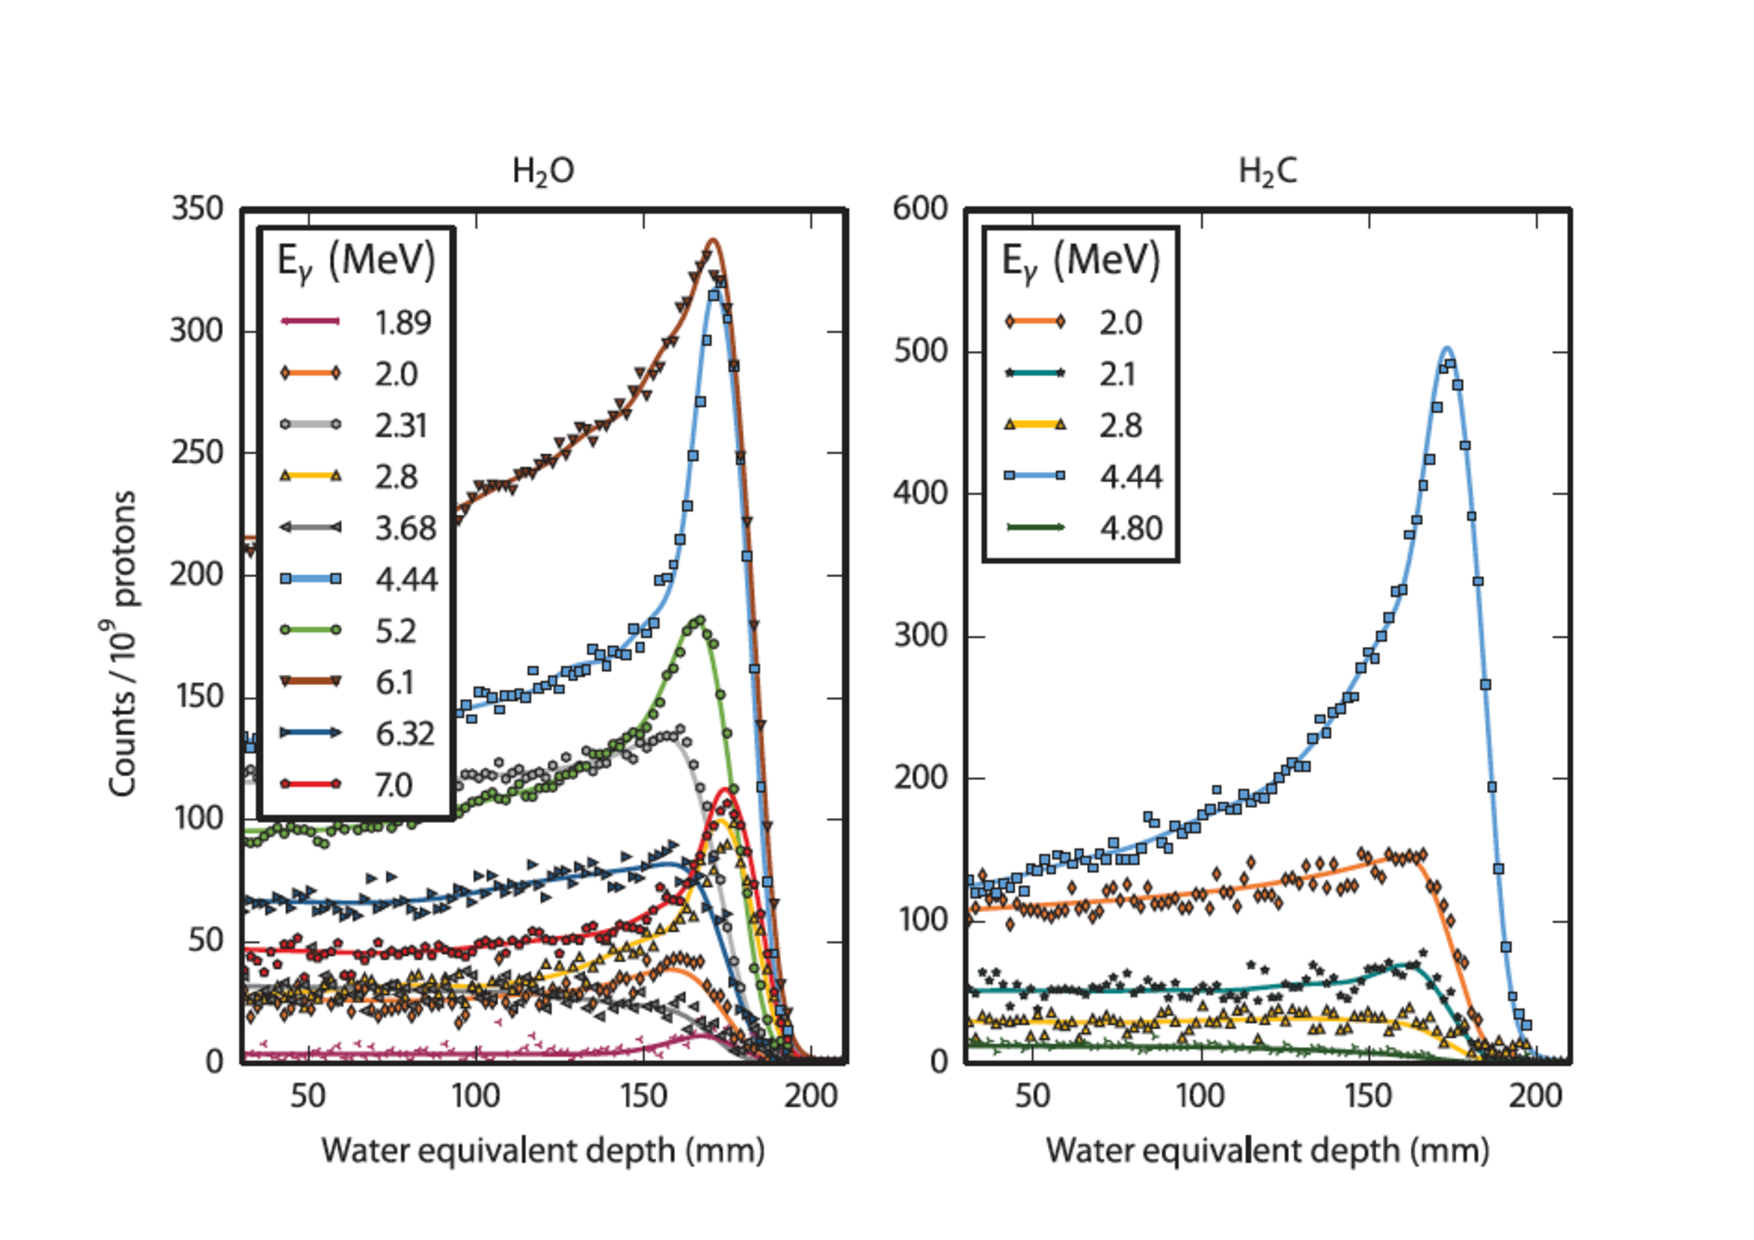
\includegraphics[width=1.2\linewidth]{03_GraphicFiles/chapter2_GammaCameras/PGS_range.pdf}
\caption{Discrete \gls{pg} spectroscopic lines along 165~MeV proton  beam stopped in water and polyethylene. The lines model the experimental data.}
\label{chap2::fig::PGS_range}
\end{subfigure}
\caption{In~\cite{Verburg2013} (left) and \cite{Verburg2014} (right).}
\label{chap2::fig::PGS_composition}
\end{figure}

A full-scale clinical prototype based on eight \gls{labr3} scintillators and an enhanced collimator design has been recently developed~\parencite{HuesoGonzalez2018}. The prototype has been tested with phantom on a proton \gls{pbs} gantry, and satisfactory performance has been obtained for a clinical beam current of 2nA incident on the phantoms. 1.1~mm precision in the measurement of the absolute proton range is stated, and tests on a ground-truth anthropomorphic head phantom~\parencite{Wohlfahrt2018} are foreseen for final validation.   

Non-imaging devices represent cost-effective solutions for range verification in particle therapy, and an extended clinical application of these methods can be expected in the next future. 

\subsubsection{Imaging prototypes}\label{chap2::subsec::PGdevices_Imaging}

With respect to non-imaging detection systems, imaging prototypes are more complex since the objective is the direct measurement of the spatial information carried by the prompt photons about their emission point. Collimation strategies are needed to retrieve spatial information, and the devices developed for particle therapy monitoring applications can be divided into mechanically and \enquote{electronically} collimated cameras. In addition to this, image reconstruction methods are needed, and are briefly presented in section~\ref{chap2::sec::Image_reconstruction}. 

\subsubsection{Mechanical collimation}\label{chap2::subsubsec::PGI_mechColl}

Mechanical collimation systems are intended to select the photons approaching the detector according to their direction, by absorbing or scattering away the undesired ones. The spatial distribution of the \gls{pg} emission points is directly retrieved along the beam path in matter, according to the specific camera \gls{fov}. The design is somehow similar to Anger cameras employed in nuclear medicine, but the collimator design has to be adapted to the \gls{pg} energy range, and the selection is generally made on a single dimension, parallel to the beam direction. As for Anger cameras, the collimator is generally coupled to high-density scintillator detectors read-out by photo-sensors.  
Several collimator geometries, with various degrees of complexity, have been tested since the beginning of the investigation of \gls{pg} as a tool for particle therapy range monitoring.
In the first \gls{pg} studies, which allowed to verify the correlation of the emission profile to the distal fall-off region, simple scintillator detectors have been placed behind parallel slit collimators~\parencite{Min2006, Min2007}. The collimator is also effective in capture fast neutrons thus reducing neutron background contamination, more pronounced with carbon-ion beams. In this case, \gls{tof} information has been used during measurements performed by the \gls{ipnl} group at \gls{ganil}, in addition to the mechanical parallel slit collimation~\parencite{Testa2008, Testa2009}. 

Parallel multi-slit configurations \myMarginnote{Multi-slit collimators} represent an improvement of such first approaches, but will require multiple or position sensitive detectors. As for Anger cameras, the presence of a passive selection system always imposes a trade-off between detection efficiency and spatial resolution, and dedicated simulation studies have been performed by the already cited groups to optimize multi-slit collimator designs~\parencite{Min2012, Pinto2014}. The collimator studied in~\cite{Pinto2014} is available at the \gls{ipnl} and composes, together with a \gls{bgo}-detector array, the collimated camera under development by the \gls{clarys} collaboration, object of this thesis work and described in details in chapter~\ref{chap::3}. The first tests on beam of a basic camera configuration has been recently performed at the \gls{cal} in Nice with 65~MeV proton beams, and the results are presented in chapter~\ref{chap::6}.   

Alternative designs include pinhole and knife-edge cameras\myMarginnote{Pinhole / Knife-edge cameras}. The pinhole design is directly derived from classical optics, and consists in a thick collimator with a tiny hole, allowing for two-dimensional imaging. The concept is adapted for the detection of \gls{pg} rays, and the collimator must be customized for the \gls{pg} energy range. Kim and colleagues designed via \gls{mc} simulations and constructed a pinhole camera based on thallium-doped \gls{csi} scintillation detectors, which has been tested with 50~MeV proton beams irradiating a water target~\parencite{Kim2009}. The camera aperture was located in proximity to the expected end point of the proton range, and 1~mm proton range variations could be detected in water. Such a collimation strategy strongly impacts the detection efficiency; for range monitoring, mono-dimensional imaging in the beam direction is sufficient, and the pinhole aperture can be extended to a knife-edge configuration, a single slit perpendicular to the beam direction and parallel to the detector plane~\parencite{Bom2012}. A knife-edge camera prototype has been optimized via \gls{mc} simulations and developed~\parencite{Smeets2012}; the tests performed on 100 and 160~MeV proton beams showed few millimeters standard deviation in the range estimate. Following these first studies, a second prototype with \gls{lyso} scintillation slabs and \glspl{sipm} have been constructed in collaboration with \gls{iba}. With such a device, shown in \figurename~\ref{chap2::fig::KE_IBA}, experimental studies have been performed with 100, 160 and 230~MeV protons on an homogeneous \gls{pmma} target, with beam currents at the nozzle exit of several nA. If compared to simulation expectations, the measured \gls{pg} profiles and a precision of 2$\sigma$ in retrieving 4~mm range shifts has been reported, with an \gls{pg} energy selection in the range 3-6~MeV~\parencite{Perali2014}. An extensive experimental study has also been performed to assess the camera performance in presence of target in-homogeneity, by using tissue equivelent inserts in a \gls{pmma} target to mimic ribs, lung air cavities and skin (adipose tissue). In most of the considered cases, the detectability of 2~mm shifts has been verified, bu the system failed in detecting range shifts in close proximity to large density gradients (for example, near air cavities or low density lung tissue)~\parencite{Priegnitz2015}. The beam must stop more than 7~mm after the cavity to detect range variations.   

\begin{figure}[!htbp]
\centering
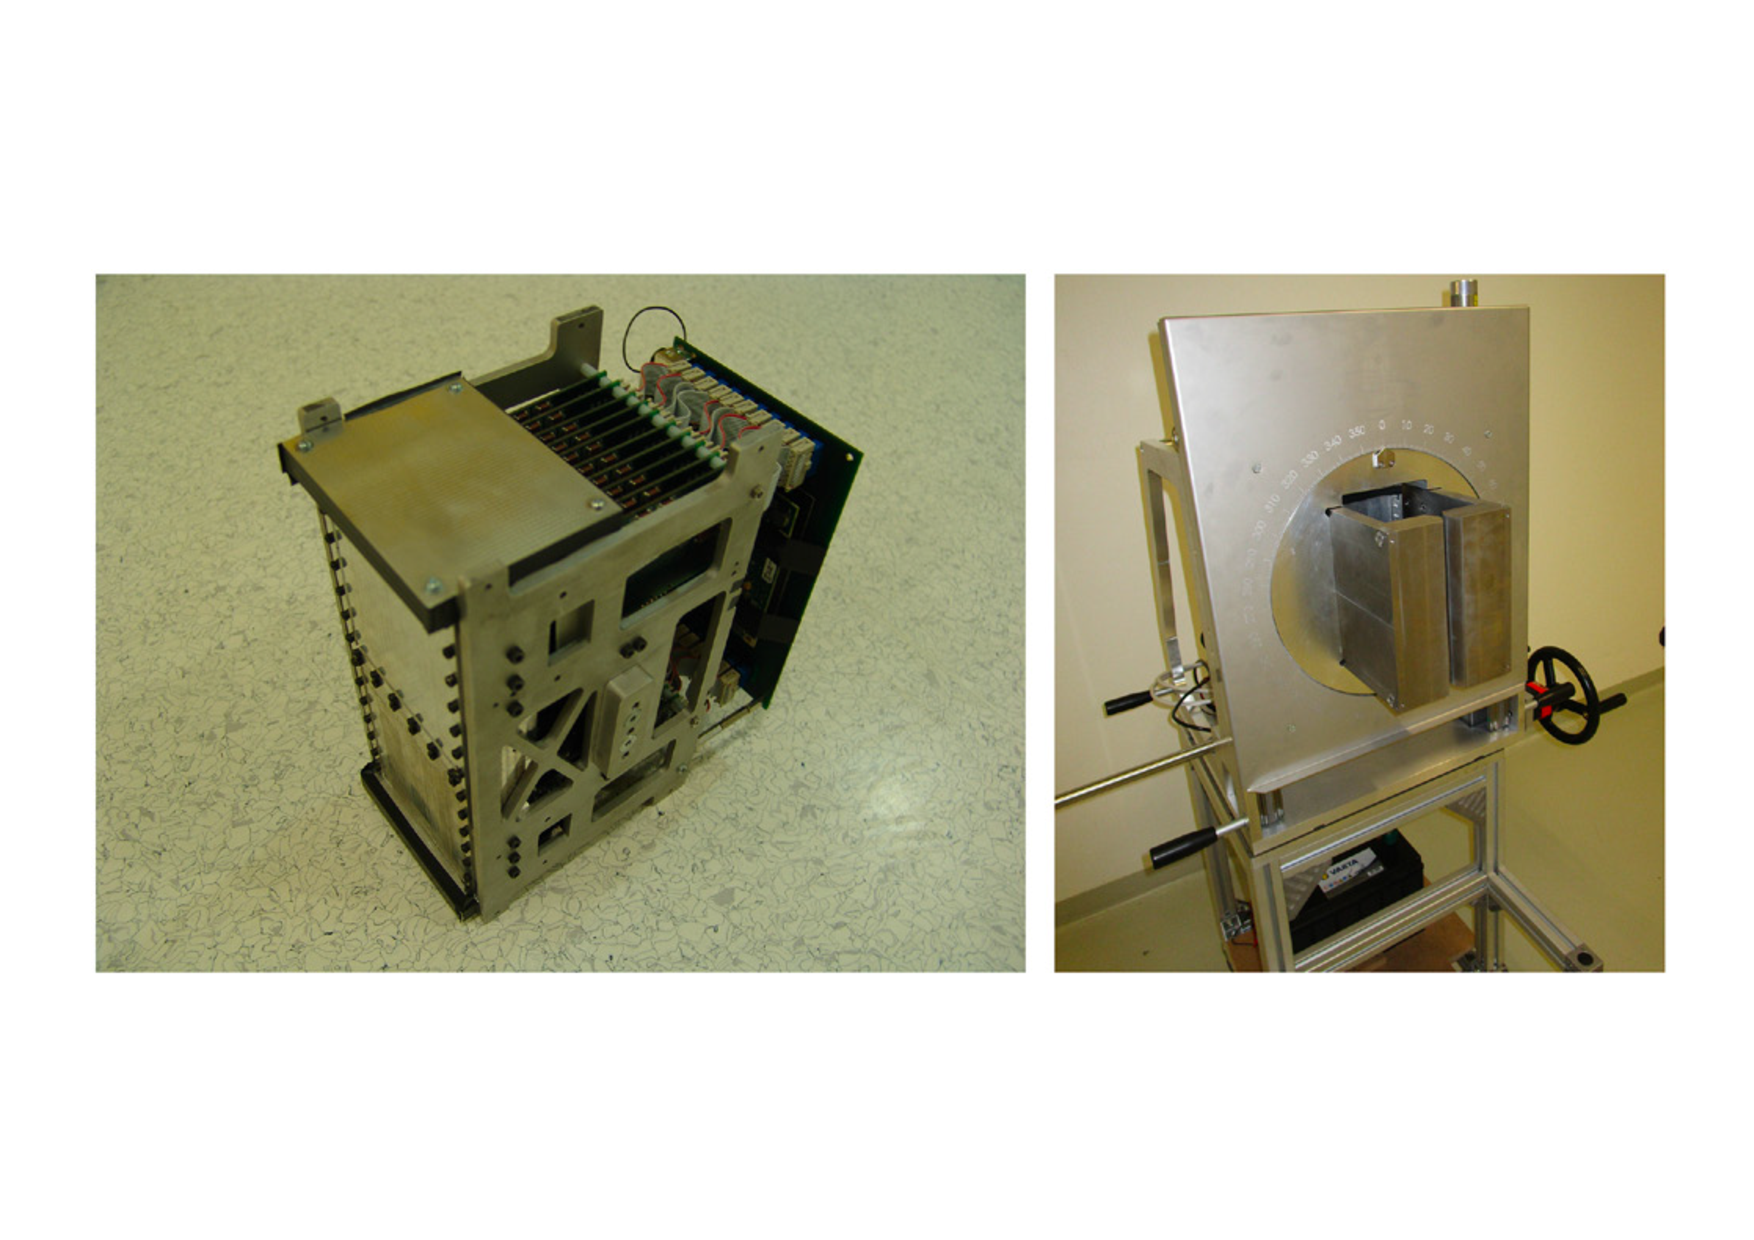
\includegraphics[width=0.9\textwidth, trim={0 3cm 0 3cm}, clip]{03_GraphicFiles/chapter2_GammaCameras/knife_edge_IBA.pdf}
\caption{\gls{lyso} slabs of the knife-edge camera (left) and complete camera with the knife-edge-shaped slit collimator mounted on a trolley. In~\cite{Priegnitz2015}.}
\label{chap2::fig::KE_IBA}
\end{figure}  

The described study only included in-homogeneity in the beam direction, but laterally in-homogeneous targets can lead to range mixing which further complicate the range detection. As highlighted in~\cite{Priegnitz2016}, in such cases the detection of range deviations strongly depends on the target composition. The combination of range deviation detection with an analysis of the slope of the distal edge of the measured \gls{pg} profile is proposed by the authors to identify the origin of the range deviation if it is due to range mixing, because range mixed \gls{pg} profiles exhibit less steep distal slopes with respect to beams traversing laterally homogeneous targets. In a further study aiming to test the clinical applicability of the knife-edge camera, it has been showed that 2-5~mm range shifts can be detected also for passive beam delivery, with the proper neutron background rejection based on preliminary un-collimated data acquisition with water targets~\parencite{Priegnitz2016}. The \gls{lyso}-\gls{sipm} detector composing the knife-edge camera have been also tested with the \gls{ipnl} multi-slit collimator (see chapter~\ref{chap::3} and ~\cite{Pinto2014}), and comparison measurements of the two configuration have been performed at the \gls{wpe} with a C230 \gls{iba} cyclotron and a \gls{pbs}-dedicated nozzle. A \gls{pmma} target has been exposed to 100, 160 and 230~MeV proton beams, and \gls{pg} profiles have been collected with the two collimator setups. The knife-edge-shaped collimator was found to be better adapted to the used camera device, because twice less protons were needed to reach a given precision in the range measurement~\parencite{Smeets2016}.
All the presented study led to the first clinical implementation of the system and, more generally, of a \gls{pg}-based monitoring device~\parencite{Richter2016}. The knife-edge camera has been used to monitor an head-and-neck tumor treatment with passive beam delivery, with the setup shown in \figurename~\ref{chap2::fig::KE_IBA_clinical}. In \figurename~\ref{chap2::fig::KE_IBA_clinical_results} the \gls{pg} profiles obtained for three iso-energy layers of the treatment, corresponding to three steps of the modulator wheel, are shown. The capability to derive spatial information of the proton range during a real treatment has been demonstrated.

\begin{figure}
\centering
\begin{subfigure}[t]{.49\textwidth}
\hspace{-0.7cm}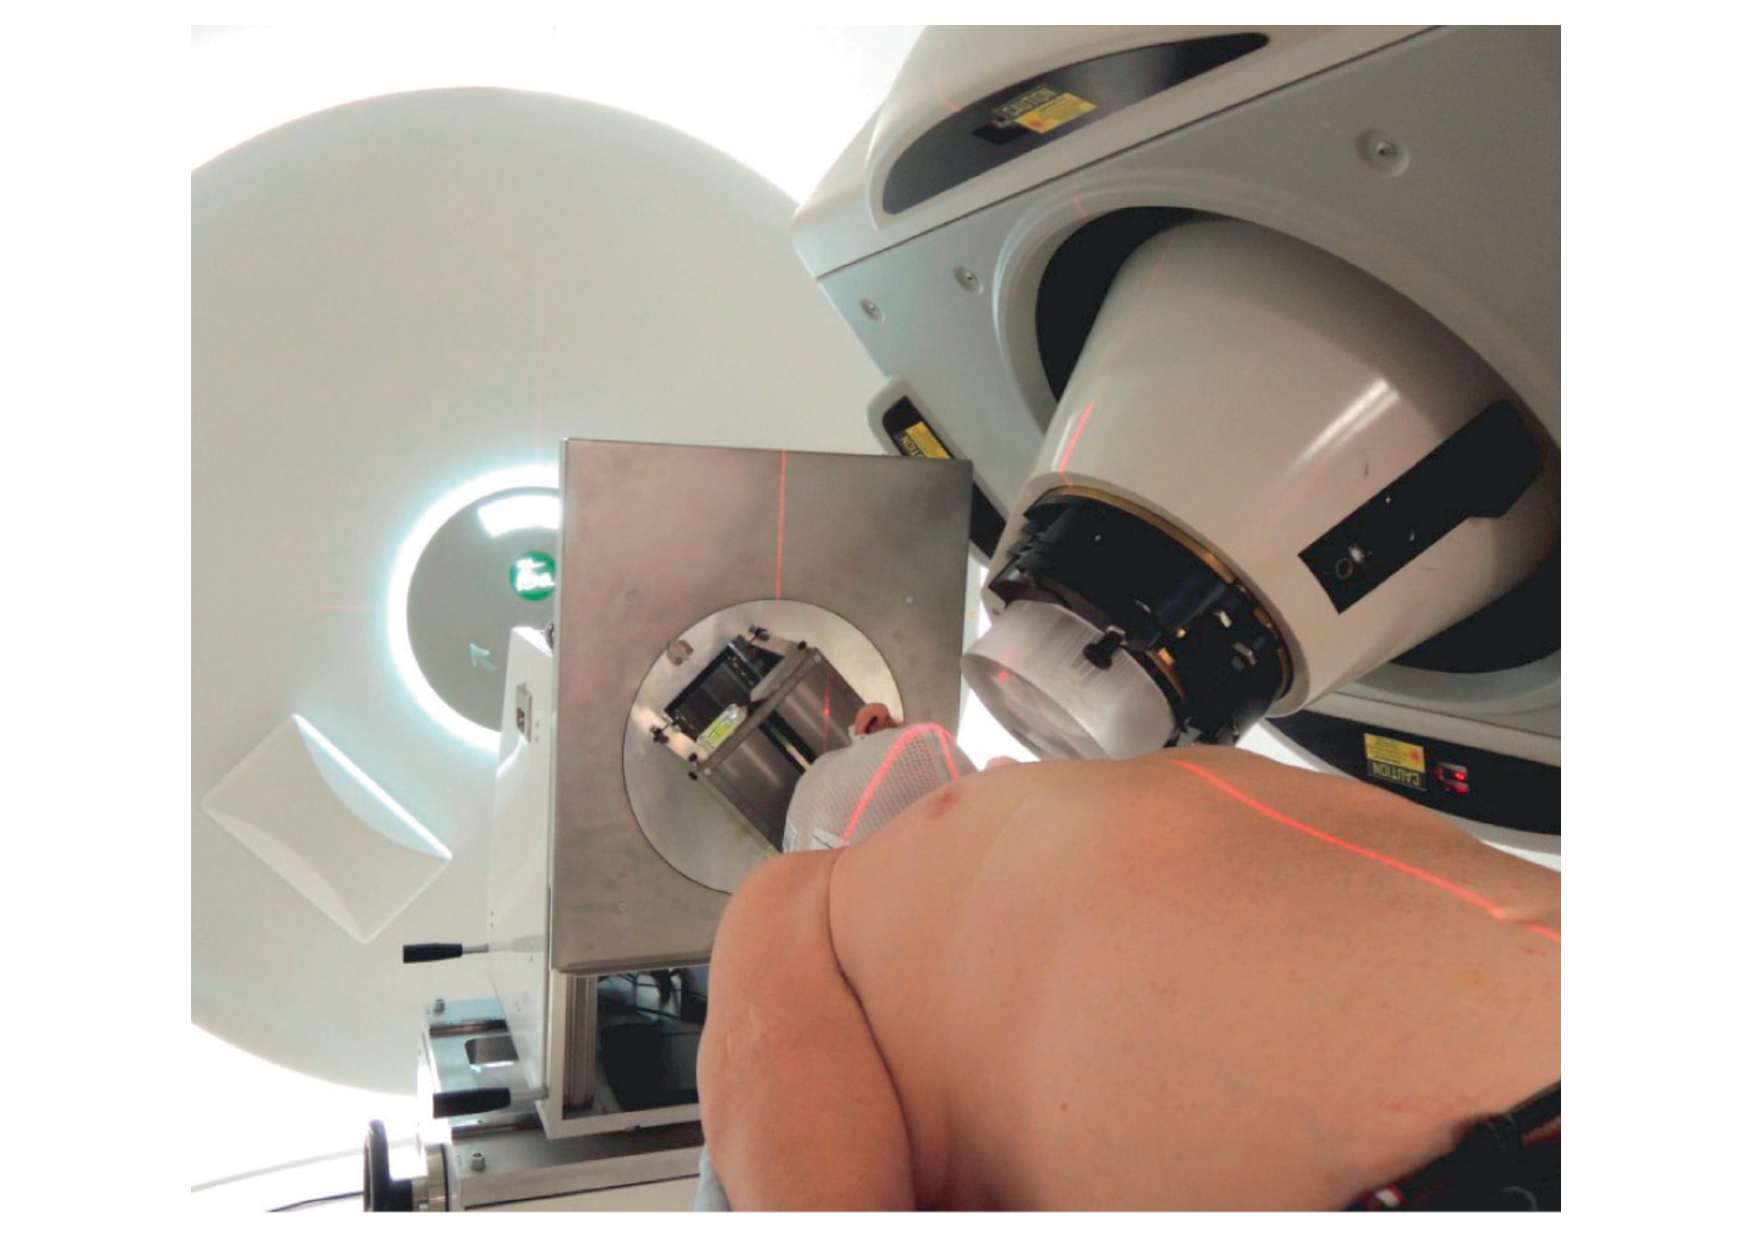
\includegraphics[width=1.2\linewidth]{03_GraphicFiles/chapter2_GammaCameras/KE_IBA_clinical.pdf}
\caption{Application of the knife-edge camera for the monitoring of the treatment of an head-and-neck tumor.}
\label{chap2::fig::KE_IBA_clinical}
\end{subfigure}
\begin{subfigure}[t]{.49\textwidth}
\hspace{-0.7cm}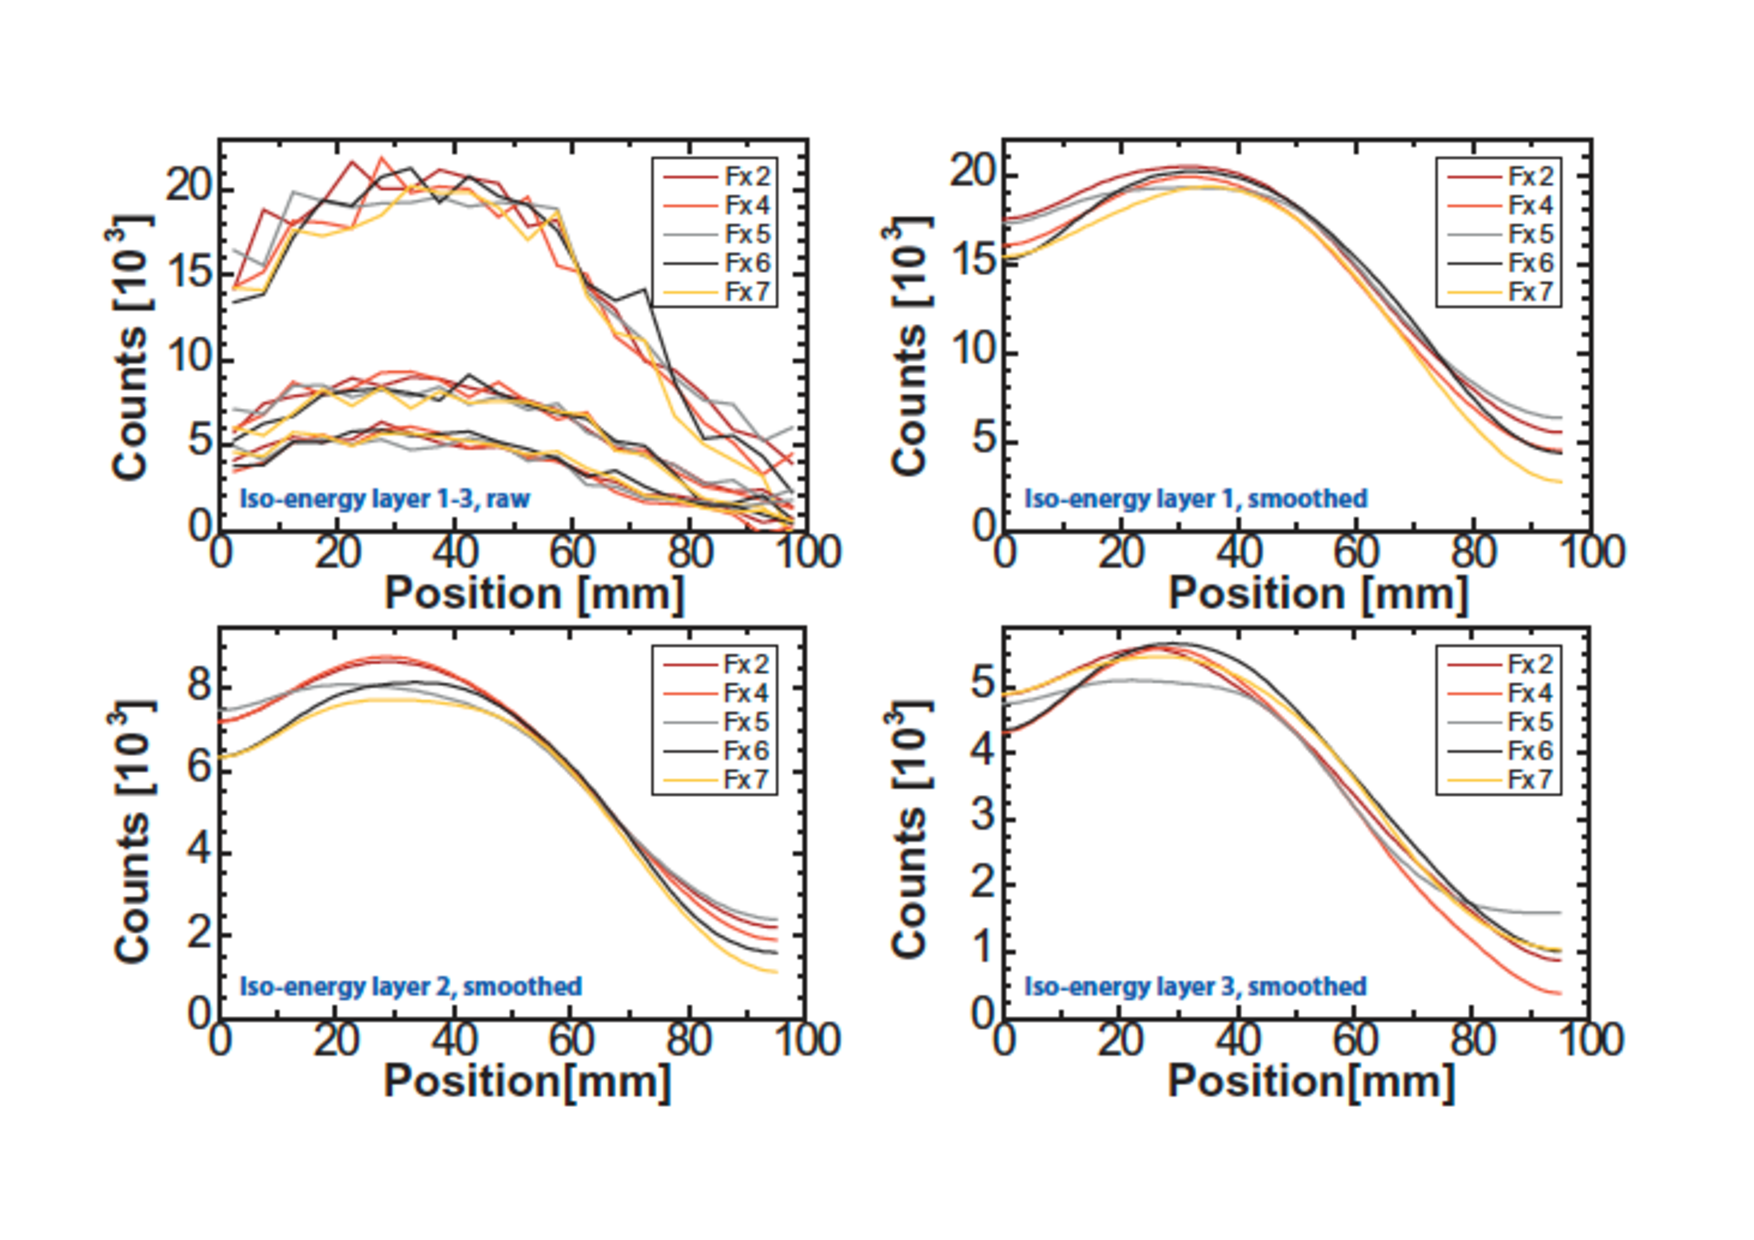
\includegraphics[width=1.2\linewidth]{03_GraphicFiles/chapter2_GammaCameras/KE_IBA_clinResults.pdf}
\caption{\gls{pg} net profiles collected during the first three iso-energy layers, corresponding to three different positions of the modulator wheel. In the first panel, the net profiles are shown. The other three panels show the Gaussian smoothed profiles of the three layers separated.}
\label{chap2::fig::KE_IBA_clinical_results}
\end{subfigure}
\caption{In~\cite{Richter2016}.}
\label{chap2::fig::KE_IBA_clinTest}
\end{figure}

A second \gls{iba} prototype has also been tested with \gls{pbs}, during 6 brain tumor treatment fraction over three weeks. Although some limitations have been identified, mainly related to the camera positioning, the possibility of spot-by-spot proton range verification has been demonstrated, with a precision of the shift retrieval depending on the number of protons in each spot. The capability of detecting range shifts below the range uncertainty margin applied in the treatment plan was also confirmed~\parencite{Xie2017}.

A two-dimensional collimated imaging solution has been designed and realized by Ready and colleagues~\parencite{Ready2016PHD, Ready2016}. It consists of a 4$\times$4 array of \gls{lso} crystals placed behind an arrangement of knife-edge slit collimators. Experimental tests have been performed by irradiating \gls{pmma} targets with a 50~MeV proton beam at currents up to 2nA, and \gls{pg} rays have been selected in the energy range 2-7~MeV. The two-dimensional \gls{pg} emission distributions have been reconstructed via \gls{mlem} algorithm and range shifts of approximately 3~mm could be detected for 10$^8$ delivered protons.   

\subsubsection{Electronic collimation: Compton cameras}\label{chap2::subsubsec::PGI_elecColl}

One of the main disadvantages of the previously described imaging system is the limited detection efficiency due to the presence of a physical collimator. In order to design imaging devices with higher statistics, the mechanical collimation has to be replaced by a so-called \enquote{electronic} collimation, which is based on Compton kinematics. In the \gls{pg} energy range the Compton effect is dominant, as shown in~\figurename~\ref{chap2::fig::relativePhotonInt}, thus can be exploited in combination with at least one more interaction to perform a sort of \enquote{photon tracking}. 
Originally designed for astrophysics applications, the potential of Compton cameras for medical imaging has been soon recognized~\parencite{Todd1974, Singh1983} and then directly translated to the ion beam therapy monitoring domain. Such a gamma detection system is generally composed of two sections: a scatterer and an absorber. The scatterer is dedicated to the gamma Compton-scattering, and should be designed to optimize the Compton scattering probability in the prompt gamma energy range, while reducing the so-called Doppler broadening effect due to electron binding and motion~\parencite{Ordonez1997} (see section~\ref{chap2::subsec::PhotonInteractions}); in most of the cases, this leads to the choice of a light material (low Z), segmented in several subsections. On the other hand, heavier materials may be used to improve photon detection efficiency. The absorber finally intends to capture the Compton scattered photons via photoelectric effect and is often composed of segmented high-Z scintillating materials. Slightly different Compton camera configurations can also achieve Compton electron tracking in the scattering detector, which results in additional information for the further reconstruction.
From the interactions points and the deposited energies in scatterer and absorber, the emission point of the incident photon can be constraint to the surface of a cone via Compton kinematics, as shown in \figurename~\ref{chap2::fig::CC_basics} for standard camera setups. Analytic or iterative algorithms use these cones to create the image of the prompt gamma emission distribution, with intrinsic three dimensional capability~\parencite{McKisson1994, Kuchment2016}. 
  
\begin{figure}
\centering
\begin{subfigure}[t]{.49\textwidth}
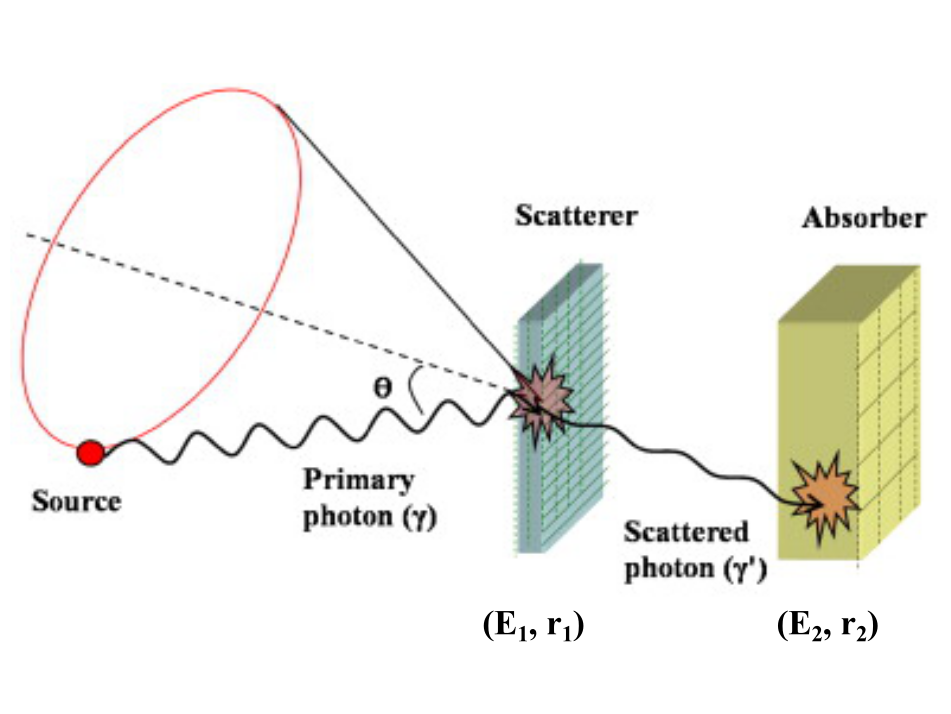
\includegraphics[width=1.0\linewidth]{03_GraphicFiles/chapter2_GammaCameras/ComptonCamera_principle.png}
\caption{Schematic view of the Compton camera detection principle for a standard camera setup.}
\label{chap2::fig::CC_detPrinciple}
\end{subfigure}
\begin{subfigure}[t]{.49\textwidth}
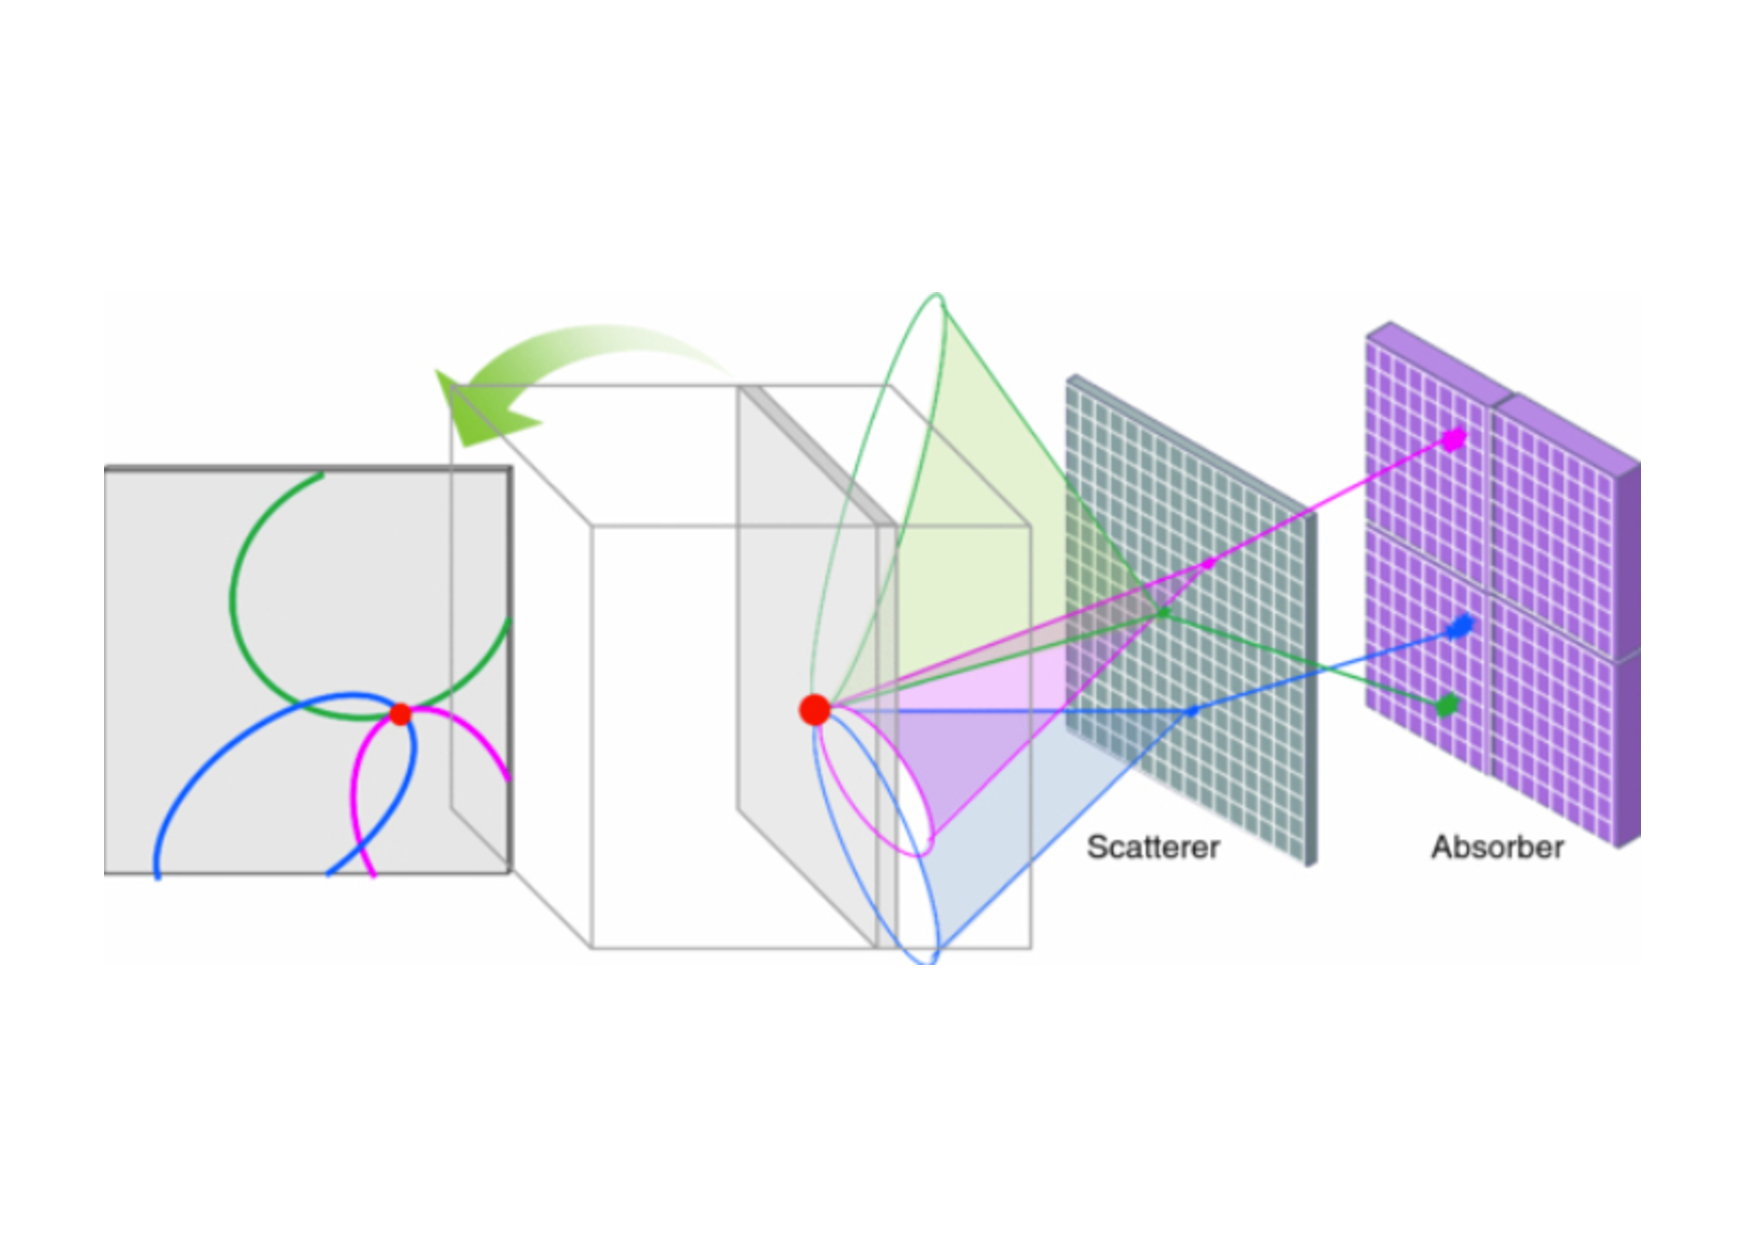
\includegraphics[width=1.0\linewidth]{03_GraphicFiles/chapter2_GammaCameras/Compton_cones.pdf}
\caption{Schematic showing a conventional Compton camera setup and reconstructed cones.}
\label{chap2::fig::CC_cones}
\end{subfigure}
\caption{Adapted from~\cite{Seo2010} (left) and in~\cite{Kim2013} (right).}
\label{chap2::fig::CC_basics}
\end{figure}

The Compton interaction position in the scatterer provides the apex of the cone, and the cone axis is given by the line connecting the interaction positions in scatterer and absorber. The cone aperture is then calculated via equation~\ref{chap2::eq::ComptonAperture}, where $E_1$ is the energy deposited in the scatterer, and $E_2$ is the energy deposited in the absorber. To be noticed that this relationship assumes that the initial photon energy ($E_0$) corresponds to $E_1 + E_2$; this means that full absorption of the photons is required for the application in \gls{pg} detection, since the energy of the incident photon is not known \textit{a priori}. 

\begin{equation}
\cos{\theta} = 1 - \frac{m_ec^2E_ 1}{E_2(E_1+E_2)} 
\label{chap2::eq::ComptonAperture}
\end{equation} 
with $m_{e}c^{2} = 511$~keV.

If at least two Compton interactions are collected in the scatterer layers, the full photon energy absorption is not necessary for the cone reconstruction, as explained in~\parencite{Kurfess2000}. The incident photon energy ($E_0$) can be calculated analytically as in equation~\ref{chap2::eq::ComptonTriple}, where $E_{1c}$ and $E_{2c}$ are the energy deposited in the two Compton scattering interactions and $\theta_{2c}$ is the Compton scattering angle related to the second interaction. 

\begin{equation}
E_0 = E_{1c} + \frac{1}{2}\bigg(E_{2c} + \sqrt{E_{2c}^2+\frac{4E_{2c}m_ec^2}{1-\cos\theta_{2c}}}\bigg) 
\label{chap2::eq::ComptonTriple}
\end{equation} 

However, the correct ordering of events is required, and limiting the data collection to multiple scattered events leads to an efficiency reduction of at least an order of magnitude~\parencite{Roellinghoff2011}.

Several research groups have developed or are developing Compton camera prototypes, following different strategies, concepts and employing various detector kinds, such as scintillators, semiconductors and gaseous detectors, as well as their combination. The application is not limited to the medical field; prototypes have been also developed for industrial monitoring, homeland security and nuclear inspections~\parencite{Martin1994, McKisson1994}. The field is in continuous progress, and in the following the state-of-the art of the prototypes already tested or under construction is presented.

Three layers of monolithic \gls{labr3} crystals \myMarginnote{Scintillators}(27.2$\times$26.8~mm$^2$ and 32$\times$36~mm$^2$ section and 5 and 10~mm thickness respectively) compose a Compton camera prototype developed in Valencia and called MACACO (see \figurename~\ref{chap2::fig::CC_MACACO}), successfully used to reconstruct point-like sources~\parencite{Llosa2016} and able to detect range shifts within 10~mm for 150~MeV proton beam impinging on a water target~\parencite{Solevi2016}. The final device followed preliminary prototypes based on a single \gls{labr3} coupled to \glspl{sipm}~\parencite{Llosa2012} and on the combination of \gls{labr3} and \gls{lyso} crystals~\parencite{Llosa2013}.

\begin{figure}
\centering
\begin{subfigure}[t]{.49\textwidth}
\hspace{-0.7cm}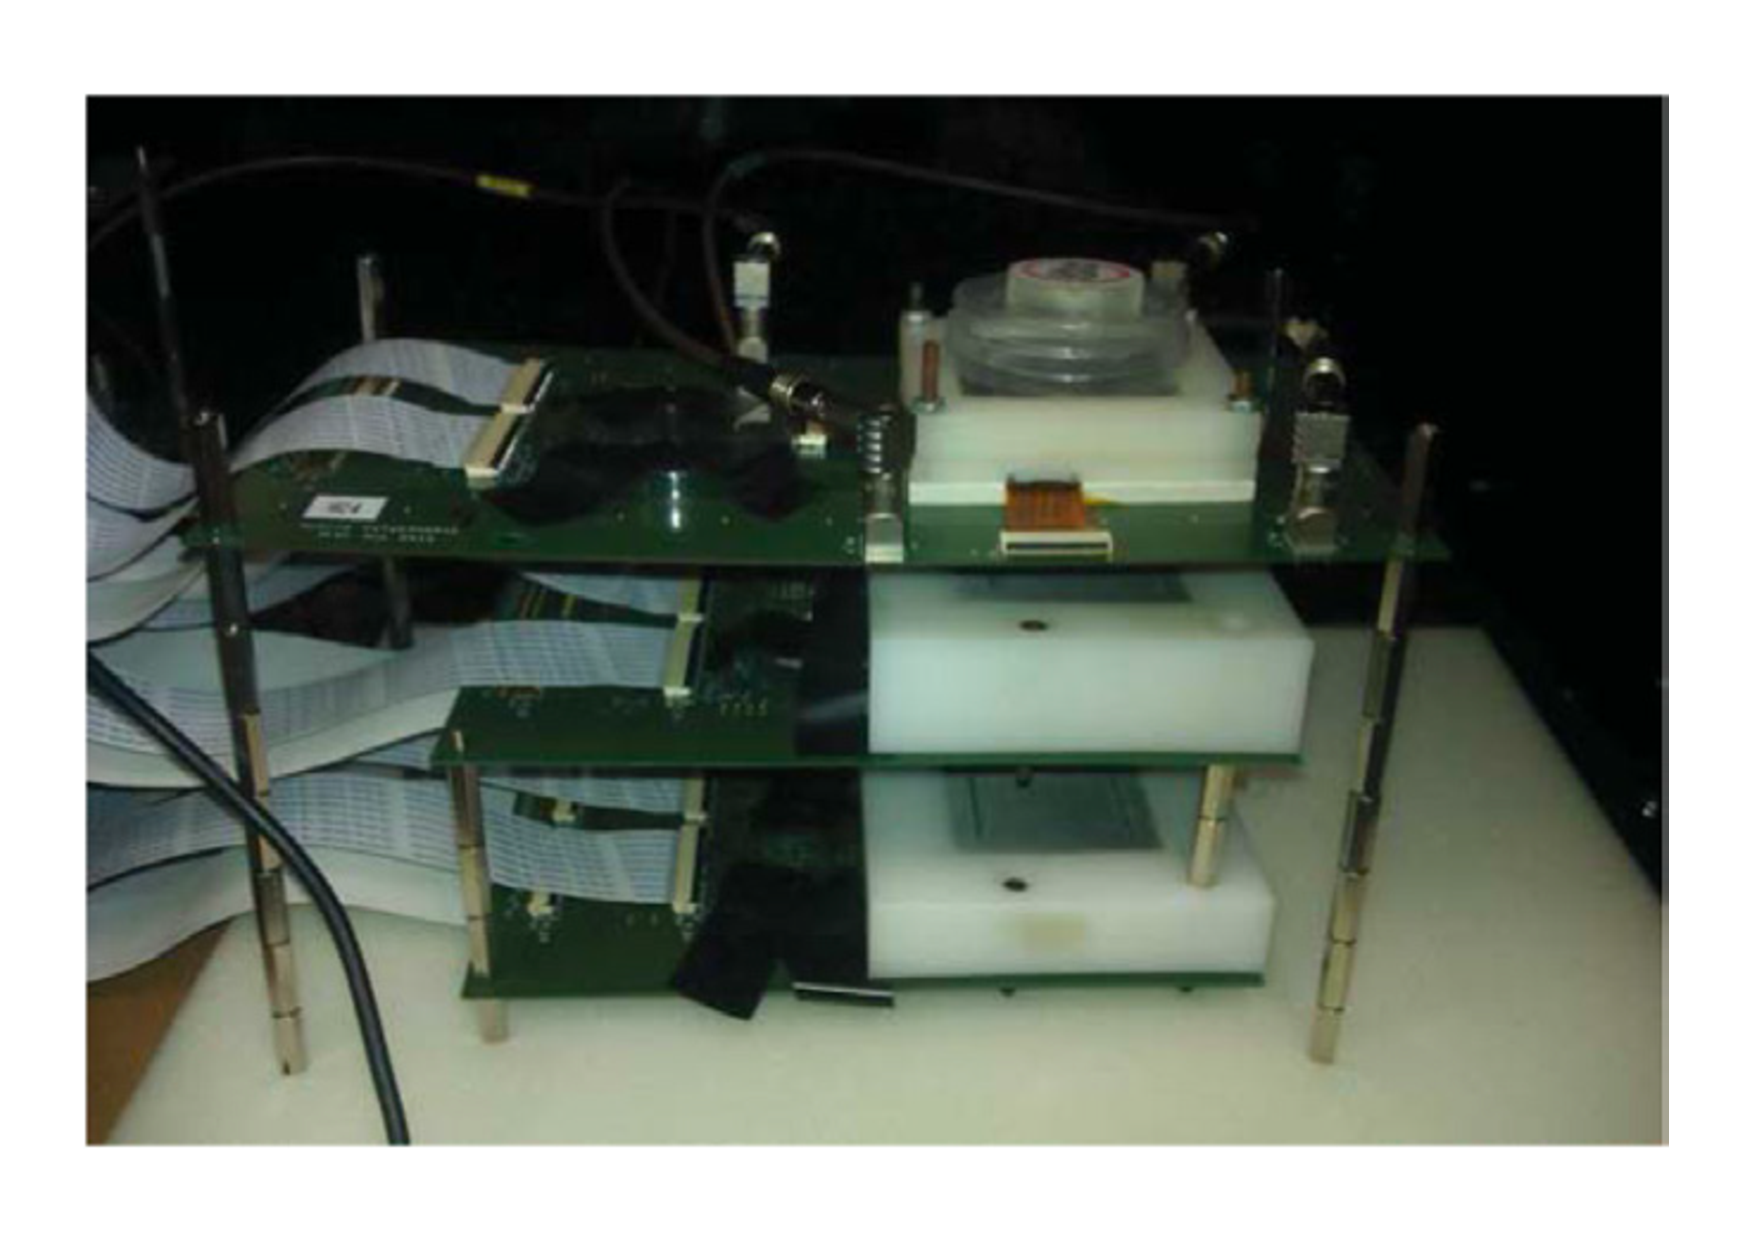
\includegraphics[width=1.2\linewidth]{03_GraphicFiles/chapter2_GammaCameras/MACACO.pdf}
\caption{Picture of the MACACO Compton prototype in a laboratory setup.}
\label{chap2::fig::CC_MACACO}
\end{subfigure}
\begin{subfigure}[t]{.49\textwidth}
\hspace{-0.7cm}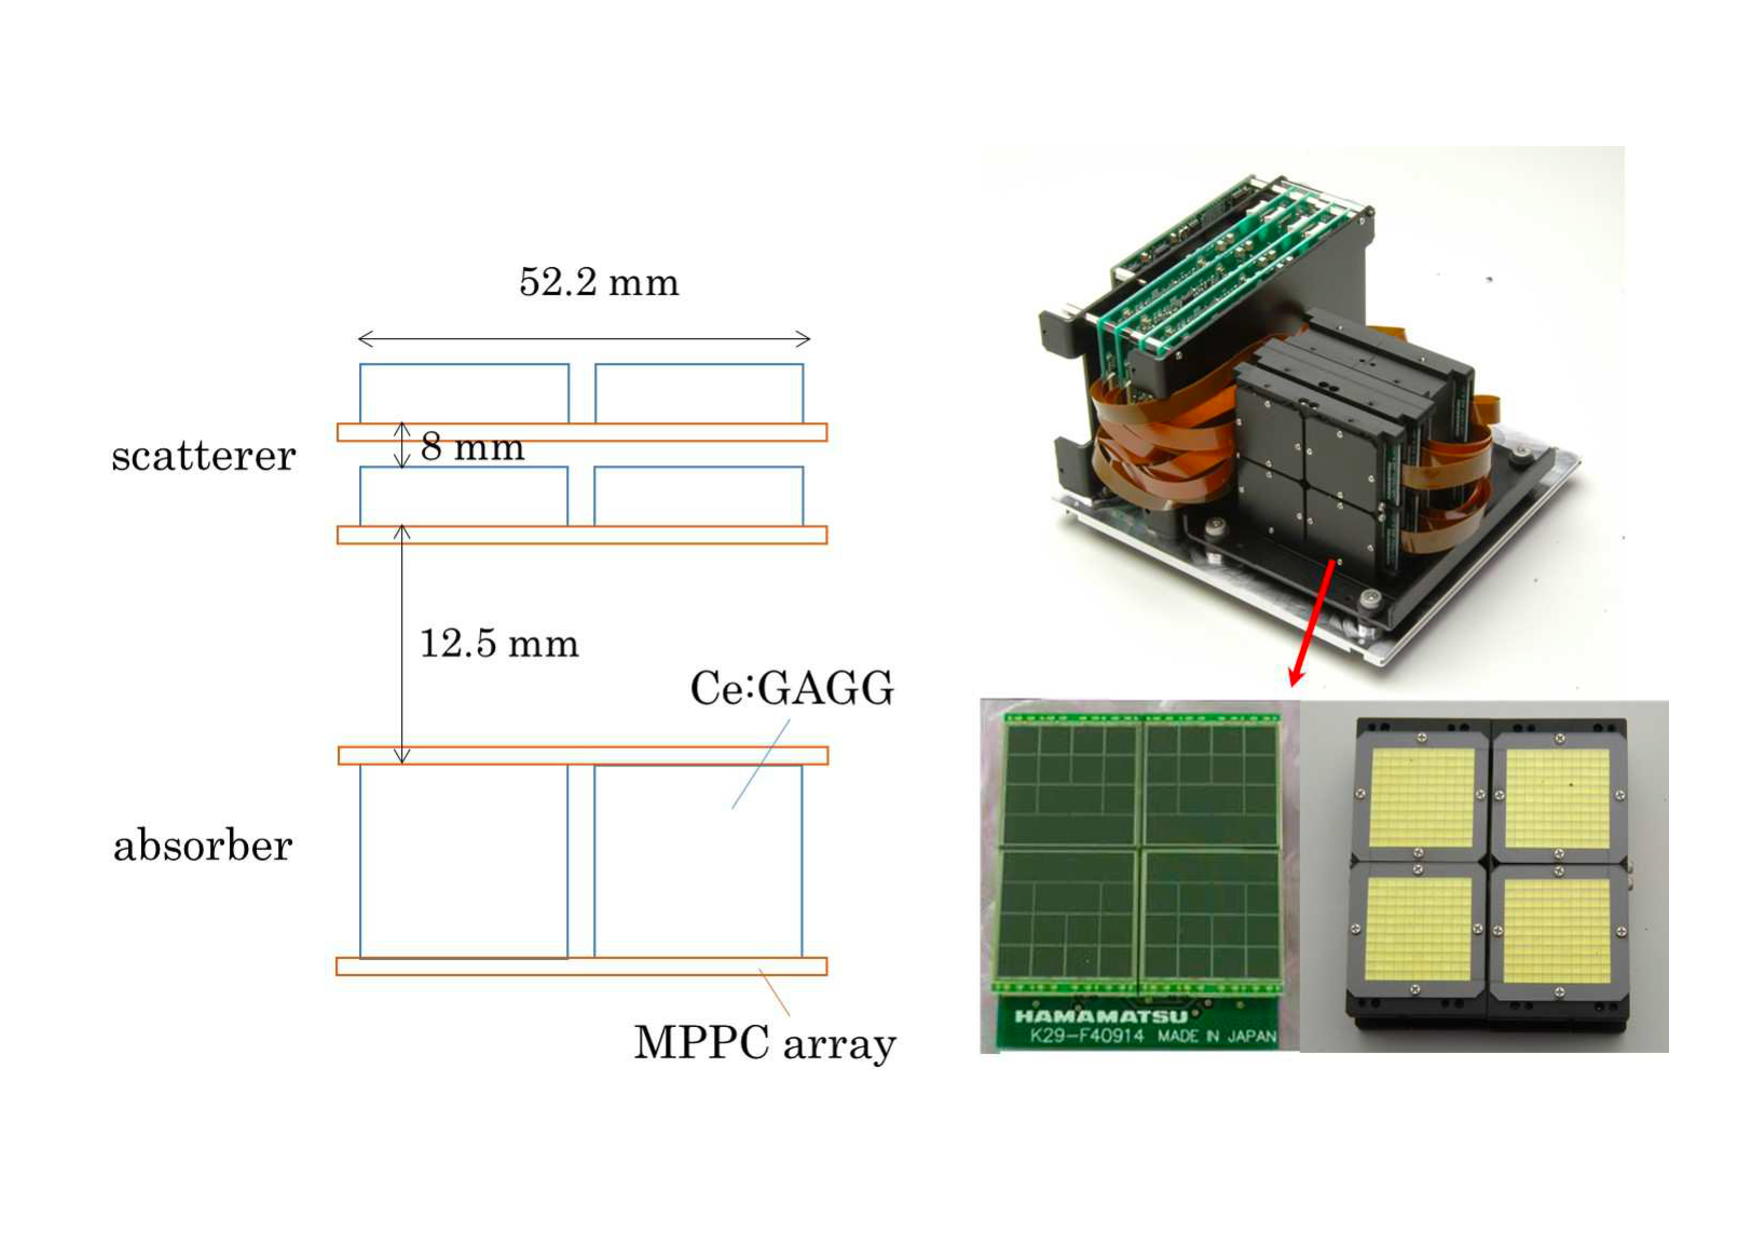
\includegraphics[width=1.2\linewidth]{03_GraphicFiles/chapter2_GammaCameras/HandheldCC.pdf}
\caption{Schematic representation and picture of an handheld Compton camera based on \gls{gaggce} scintillators.}
\label{chap2::fig::CC_handheld}
\end{subfigure}
\caption{In~\cite{Solevi2016} (left) and in~\cite{Kishimoto2015} (right).}
\label{chap2::fig::CC_scintillators}
\end{figure}

A handheld Compton camera prototype based on \gls{gaggce} scintillators has been developed~\parencite{Kishimoto2015}. The prototype is shown in \figurename~\ref{chap2::fig::CC_handheld}. Such a device was originally designed to measure radioactive isotopes such as $^{137}Cs$, that were released during and after the Fukushima nuclear disaster in 2011. The device showed a spatial resolution in the reconstruction of point-like source emissions below 7~mm~\parencite{Kishimoto2015}. Its application to particle range monitoring has been tested with 70~MeV protons on water, \gls{pmma} and Ca(OH)$_2$ targets: significant uncertainties in the determination of the Bragg peak position determined the planning of an improved performance version of the system~\parencite{Taya2016}.

With the aim of maximizing the ratio between \myMarginnote{Semiconductors and scintillators}Compton and photoelectric absorption probabilities in the scatterer and, at the same time, reducing the Doppler broadening effects, semiconductor detectors have been considered in several prototypes, coupled to high-Z scintillators for the absorber. The Compton camera developed by the \gls{clarys} collaboration, main object of this thesis, is based on this idea and employs 7 \glspl{dssd} for the scatterer stack, coupled to an array of \gls{bgo} blocks as absorber~\parencite{Krimmer2015, Fontana2018}. A beam tagging hodoscope based on scintillating fibers is also included in the development program~\parencite{Krimmer2014}. A complete description of the camera components and the present status of the development is given in chapter~\ref{chap::3}. The most recent results obtained in simulation studies concerning the application of such prototype to particle therapy range monitoring and nuclear medicine are presented in chapter~\ref{chap::4} and chapter~\ref{chap::5}, respectively. 
The 2~mm thick silicon planes chosen for the scatterer section have been optimized to maximize the probability of stopping the Compton recoil electron within the same layer where the photon Compton interaction took place. As mentioned, the tracking of the Compton recoil electron gives additional information for the event reconstruction stage; the direction of the incident photon can be confined from the full cone to an arc.~\parencite{Frandes2010}. The possible exploitation of this imaging advantage is explored in the prototype developed in Munich by Thirolf and colleagues. The design concept is similar to the one proposed by the \gls{clarys} collaboration: a monolithic cerium-doped  \gls{labr3} scintillator crystal, 50$\times$50$\times$30~mm$^3$, used as absorber, is coupled to six \gls{dssd} layers 50$\times$50$\times$0.5~mm$^3$. The reduced thickness allows for the tracking of the recoil electron, with an increased escape probability. The absorber scintillator is read out via a 256-fold segemented multianode \gls{pm}; an energy resolution of 3.8\%  \gls{fwhm} has been reported at 662~keV, with a timing resolution of 270~ps~\parencite{Thirolf2016}.  An algorithm based on the k-nearest neighbor method is implemented for the position reconstruction~\parencite{vanDam2011}, and its \gls{cap} version has been verified to provide the best results~\parencite{Aldawood2017}. The algorithm is based on pre-determined spatially dependent detector response, and has been recently further improved with artifact correction capabilities; the new \gls{cgdr} algorithm has been used to obtain a spatial resolution below 3~mm at 1.3~MeV~\parencite{Liprandi2017}. 
A further electron-tracking Compton prototype based on a \gls{soi} pixel detector and a \gls{gaggce} detector has been developed and is described in~\cite{Yoshihara2017}. It has been conceived for the localization of contamination nuclides inside the Fukushima Daiichi Nuclera Power Plant in Japan, and two dimensional imaging of a $^137$Cs source has been demonstrated. The application of such an imaging device in nuclear medicine has been suggested by the authors, and its implementation in the monitoring on therapeutic beam range is not excluded. 
Various Compton camera prototypes make use of \gls{czt} as alternative to silicon detectors. In~\cite{Kormoll2011} the design study of a Compton camera composed of a \gls{czt} detector as scatterer (20$\times$20$\times$5~mm$^3$, 16 strips per plane) and a streaked \gls{lso} crystal as absorber (52.7$\times$52.7$\times$20~mm$^3$) is presented. The scatterer section showed a time resolution of 2.8~ns \gls{fwhm}, while a 0.6~ns resolution was reported as a result of tests performed with bremsstrahlung photons (up to 13~MeV) at the ELBE electron accelerator in Germany~\parencite{HuesoGonzalez2014}. The same authors presented a direct comparison of \gls{lso} and \gls{bgo} detectors for the detection of photons in the \gls{pg} energy range~\parencite{HuesoGonzalez2015}; although less performing than \gls{lso}, \gls{bgo} is an interesting alternative given the absence of internal radioactivity which reduce the amount of fake events contributing to the background (random coincidences). Moreover, its much lower prize makes it suitable for commercial devices. 
In addition to the \gls{clarys} collaboration prototype which includes \gls{bgo} blocks for the absorber section, a Compton camera coupling three \gls{bgo} crystals (52.7$\times$52.7$\times$20~mm$^3$) and a \gls{czt}-based scatterer has been tested with 4.44~MeV photons~\parencite{Golnik2016}. The \gls{bgo} crystals have been calibrated in energy on a single pixel-basis, with a method presented in~\parencite{HuesoGonzalez2015}, and an energy resolution of 27\% \gls{fwhm} has been found. 
Such a method has been refined and extended for the characterization measurements published in~\parencite{Fontana2018} and described in chapter~\ref{chap::3} for the \gls{clarys} \gls{bgo} blocks. 
A different approach has been first studied in simulation by Kim and colleagues, referred to as \gls{gevi}~\parencite{Kim2012, Kim2012ERR}, and then translated into a prototype. The concept relies on the passive conversion of \gls{pg} rays to electrons, that are then tracked. The developed prototype consists of a 1~mm thick beryllium plate to convert the incident photons into electrons; the electron tracker is then composed of two \gls{dssd} layers, 50$\times$50~mm$^2$ surface, 150 and 300~\charmu m thick, respectively.The kinetic energy of the electrons is then collected by a plastic-scintillator calorimeter~\parencite{Lee2017}. A $^90$Sr source has been employed to test the electron detection performance, replacing the beryllium converter; a spatial resolution of 16~mm \gls{fwhm} for the reconstruction of the point-like source has been obtained. With the converter, photons from a $^60$Co source have been used, and the obtained spatial resolution was 35~mm \gls{fwhm}. The present prototype is equipped with an acquisition system with limited rate acceptance, and tests with 45~MeV protons impinging on a \gls{pmma} target showed a very low sensitivity of 4$\times$10$^{-8}$~\parencite{Lee2017}.   

\begin{figure}
\centering
\begin{subfigure}[t]{.49\textwidth}
\hspace{-0.7cm}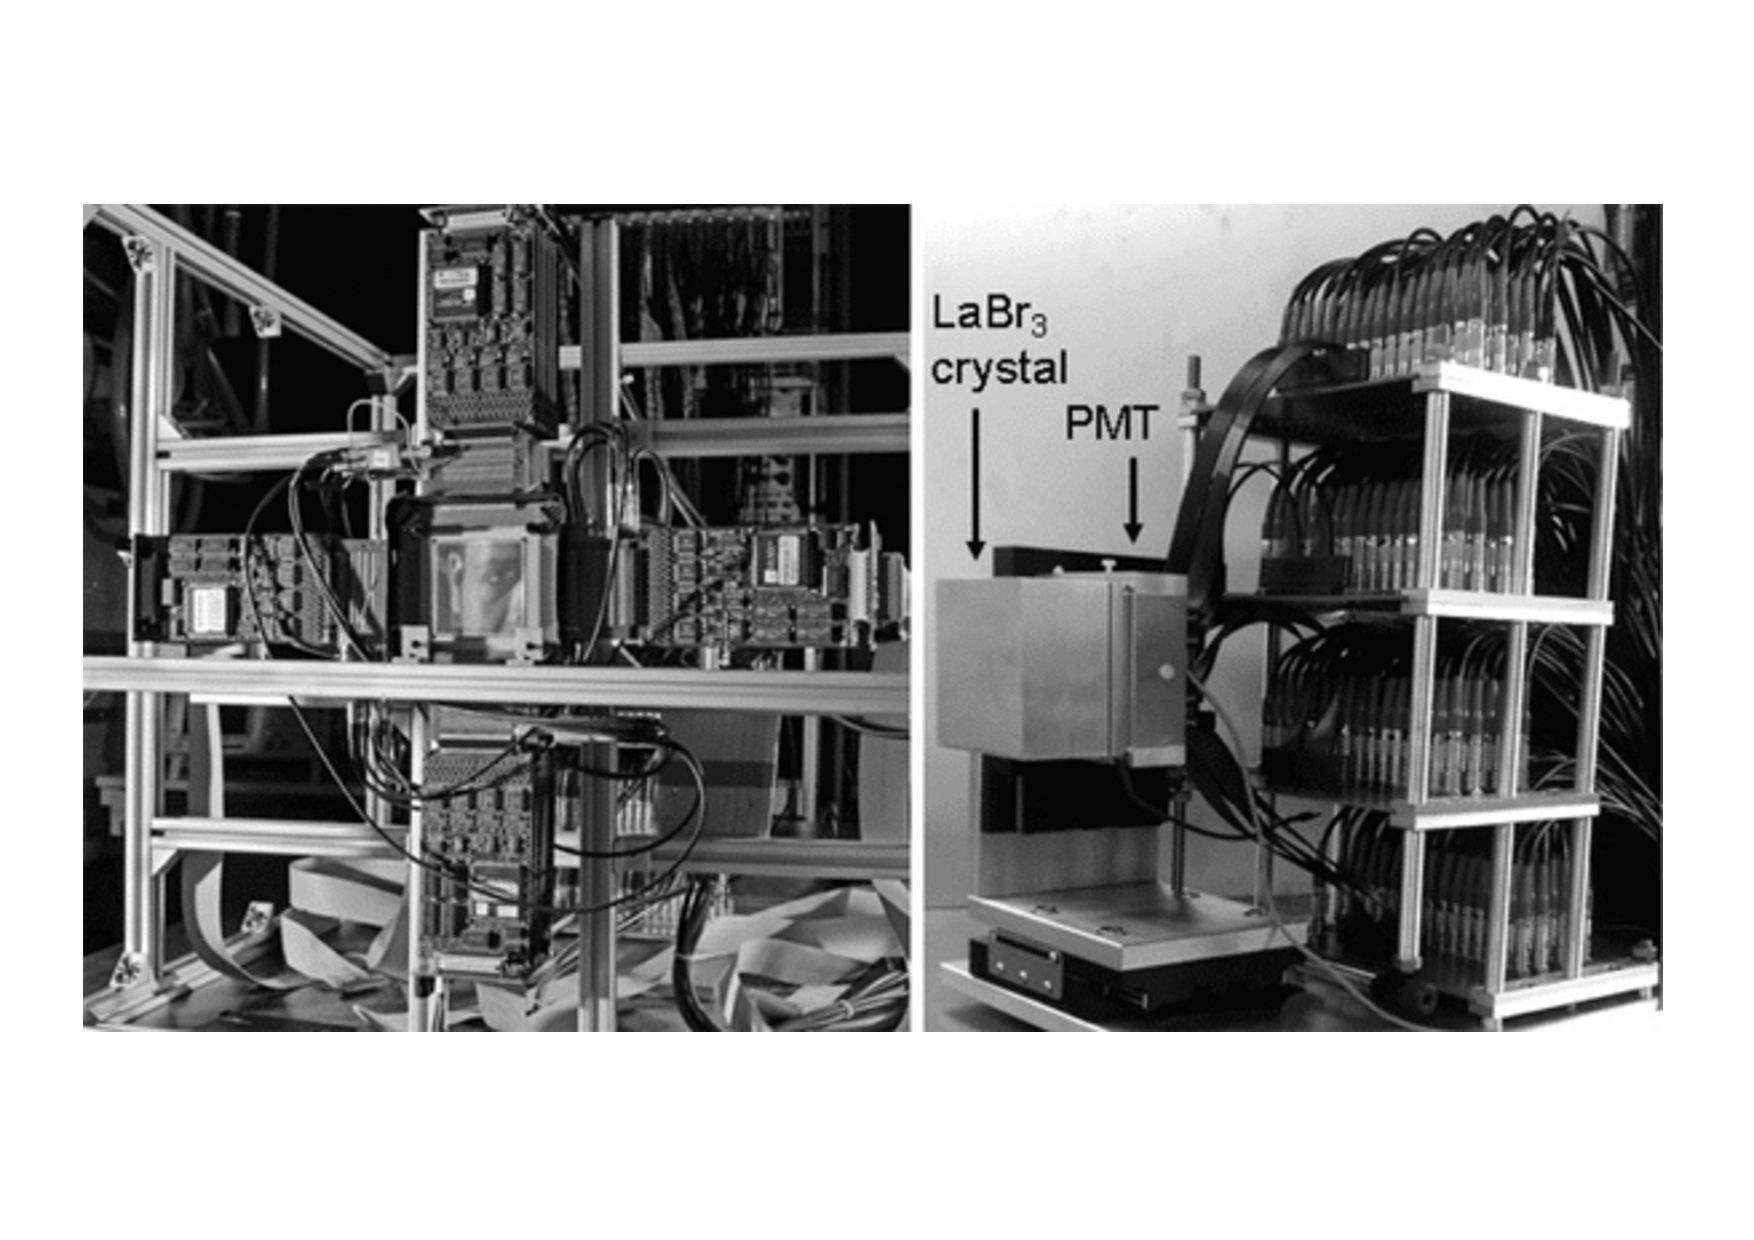
\includegraphics[width=1.2\linewidth]{03_GraphicFiles/chapter2_GammaCameras/CC_Munich.pdf}
\caption{Layout of the Munich electron tracking Compton camera.}
\label{chap2::fig::CC_Munich}
\end{subfigure}
\begin{subfigure}[t]{.49\textwidth}
\hspace{-0.7cm}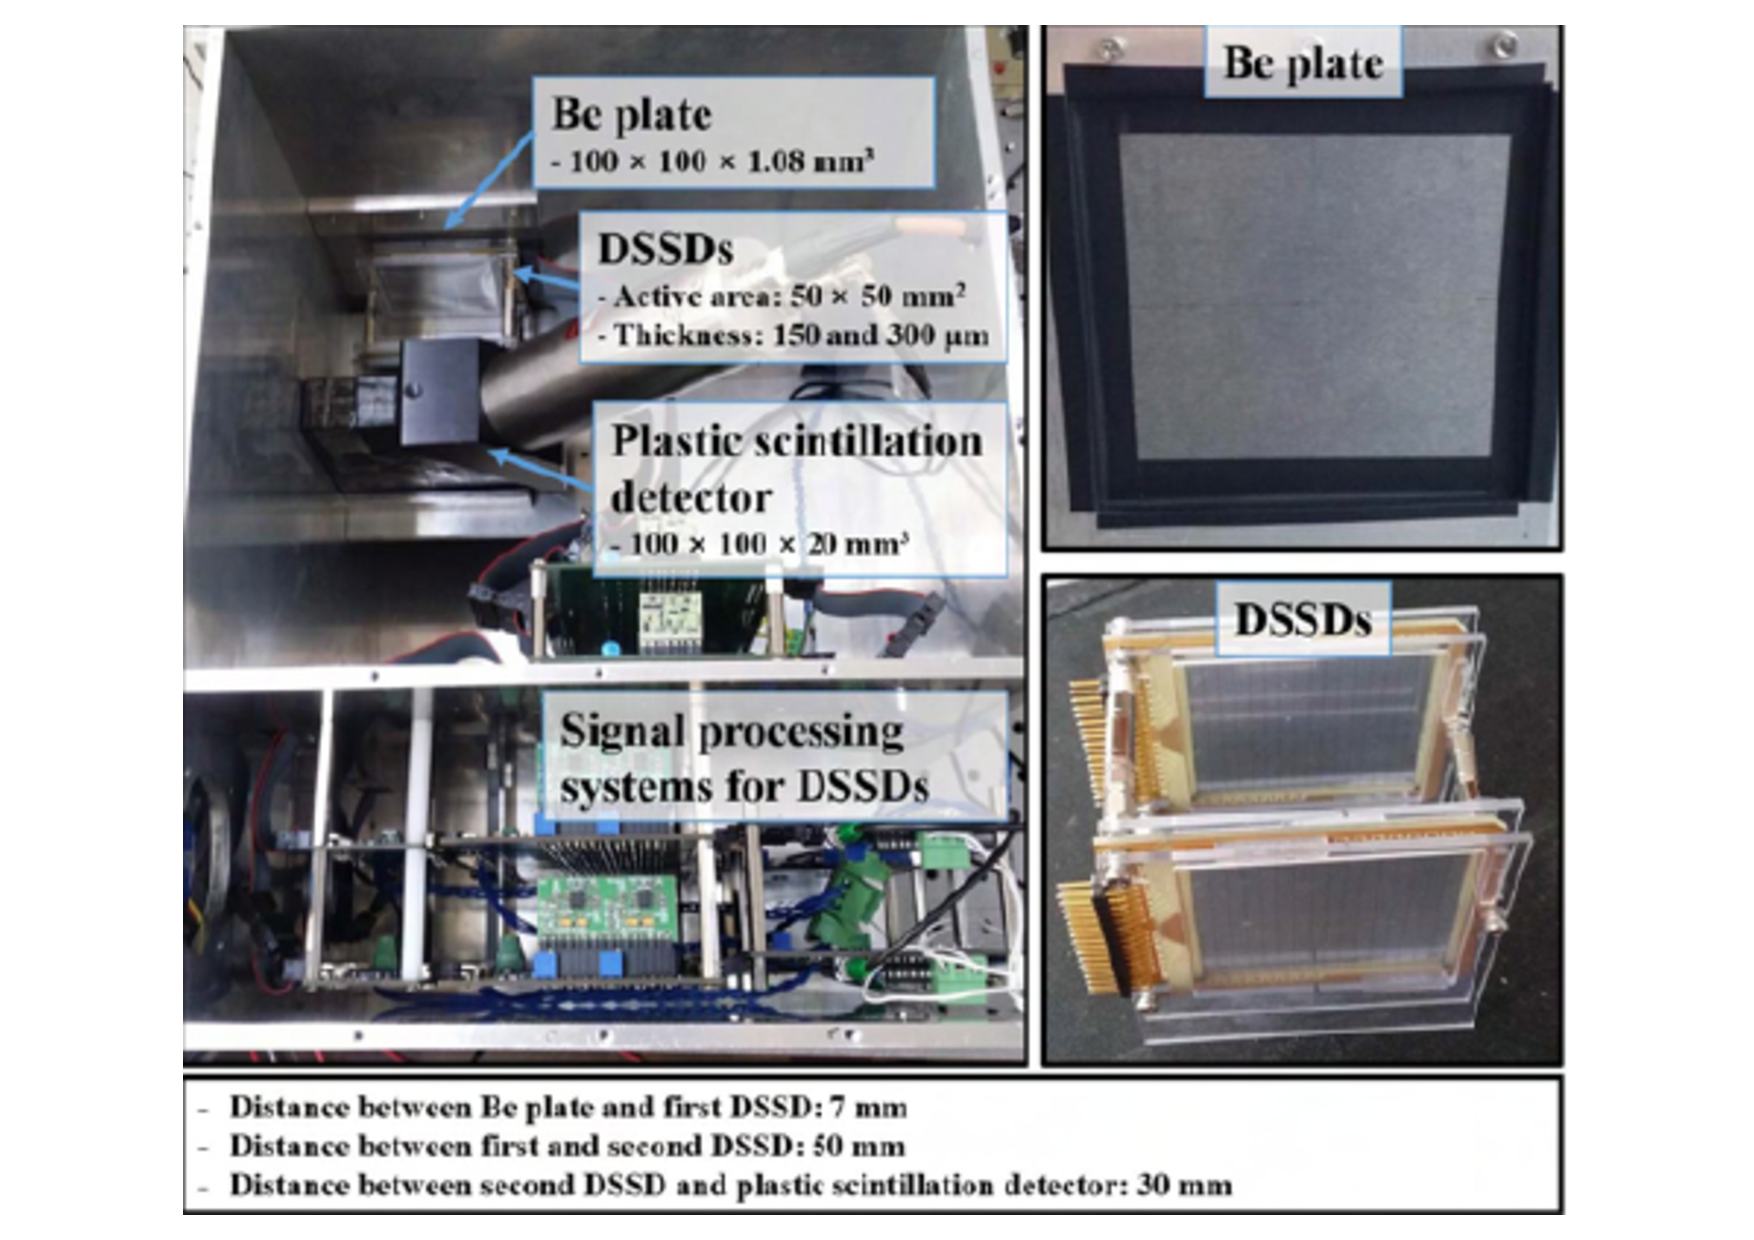
\includegraphics[width=1.2\linewidth]{03_GraphicFiles/chapter2_GammaCameras/CC_GEVI.pdf}
\caption{Components of the \gls{gevi} prototype.}
\label{chap2::fig::CC_GEVI}
\end{subfigure}
\caption{In~\cite{Thirolf2016} (left) and in~\cite{Lee2017} (right).}
\label{chap2::fig::CC_scintiSemicon}
\end{figure}

Compton camera completely based on semiconductor\myMarginnote{Semiconductors only} detectors have also been explored. Simulations studies have been published in~\parencite{Peterson2010} a presents the design optimization of a three-stage Compton camera based on germanium detectors. In addition, different materials have been investigated~\parencite{Robertson2011}, and the influence of Doppler broadening have been analyzed in details~\parencite{Mackin2013}. 
Following the simulation results, a prototype only based on \gls{czt} detectors have been constructed, named Polaris-J Compton Camera: it consists of four pixelated detectors with 20$\times$20~mm$^2$ surface for 10 and 15~mm thickness~\parencite{McCleskey2015}. The camera showed an absolute efficiency in detecting gammas from a $^60$Co source of 2.2$\times$10$^{-5}$ and 5.8$\times$10$^{-7}$ for double and triple scatter events, respectively. Clinical proton beams of 114 and 150~MeV on a water target have been used to test the feasibility of range verification, and 3~mm range shifts could be detected with one-dimensional profile analysis~\parencite{Polf2015}. The experimental setup is shown in figure~\ref{chap2::fig::CC_Polaris}.

\begin{figure}
\centering
\begin{subfigure}[t]{.49\textwidth}
\hspace{-0.7cm}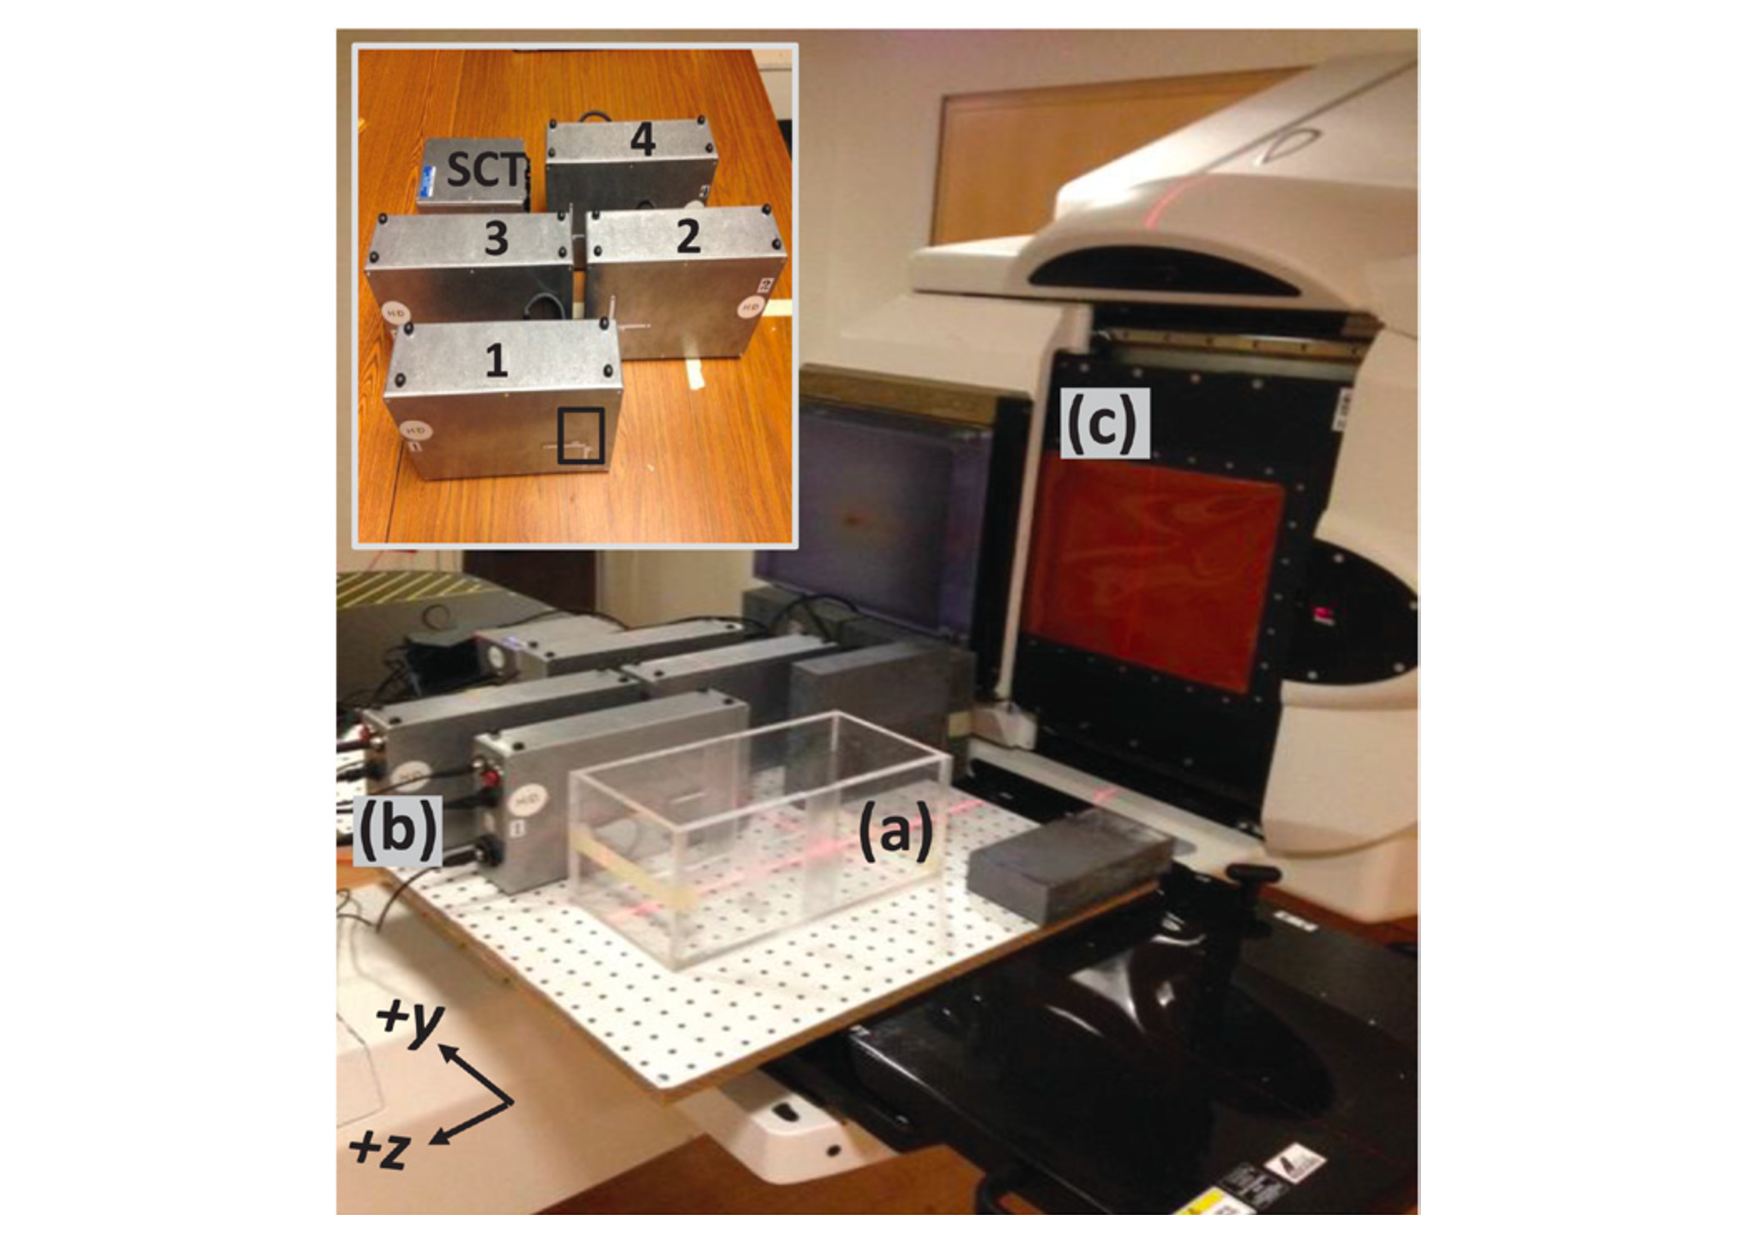
\includegraphics[width=1.2\linewidth]{03_GraphicFiles/chapter2_GammaCameras/CC_Polaris.pdf}
\caption{Experimental setup for the beam tests of the Polaris-J Compton camera (b) with a water target (a). The box in the top left side shows a close up view of the four \gls{czt} detector stages.}
\label{chap2::fig::CC_Polaris}
\end{subfigure}
\begin{subfigure}[t]{.49\textwidth}
\hspace{-0.7cm}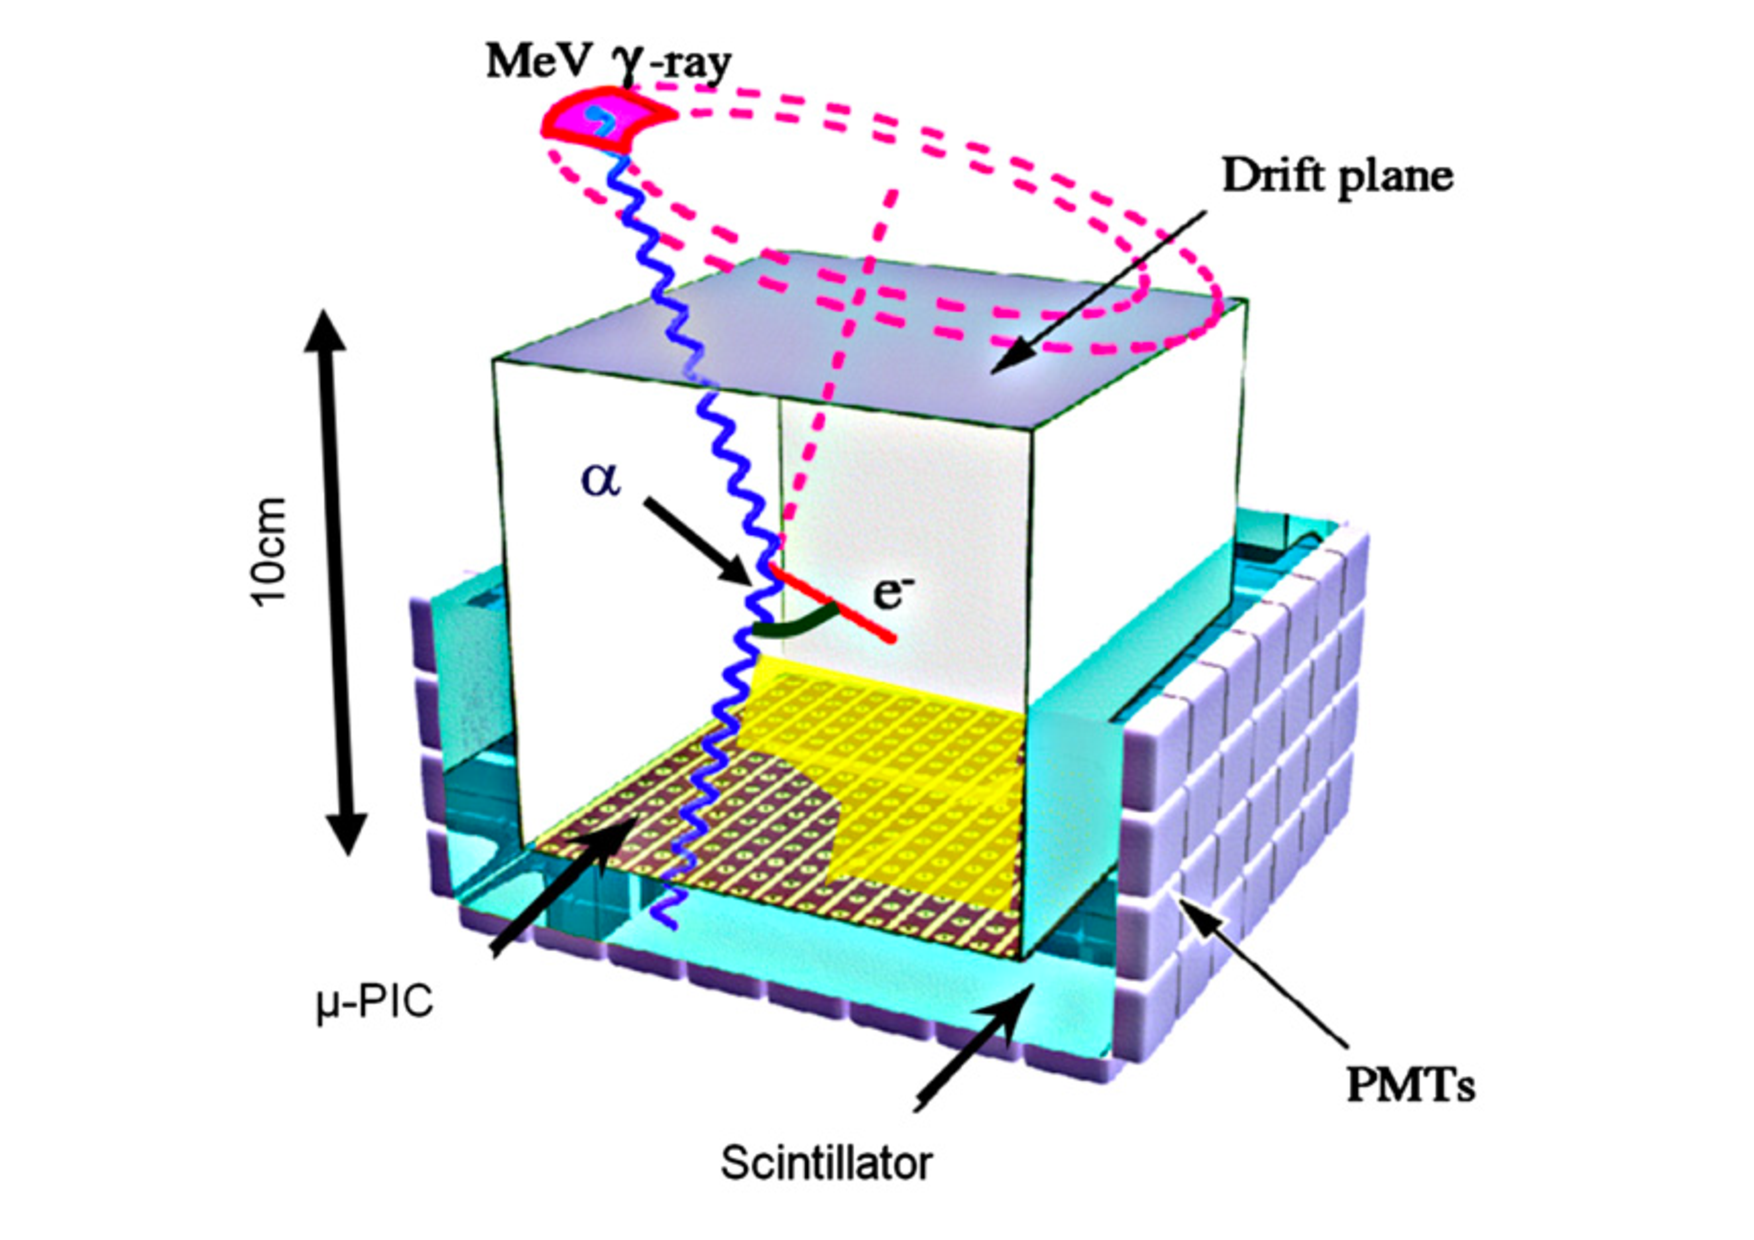
\includegraphics[width=1.2\linewidth]{03_GraphicFiles/chapter2_GammaCameras/CC_TPC.pdf}
\caption{Schematic view of the prototype and operation principle of the ETCC.}
\label{chap2::fig::CC_TPC}
\end{subfigure}
\caption{In~\cite{Polf2015} (left) and in~\cite{} (right).}
\label{chap2::fig::CC_SemiconGas}
\end{figure}

Gaseous detectors can also be applied to Compton imaging\myMarginnote{Gaseous detectors}. An electron tracking Compton camera (ETCC) has been proposed by Takada and colleagues, originally for astrophysics applications in baloon experiments~\parencite{Takada2011}. A gaseous \gls{tpc} (10$\times$10$\times$15~cm$^3$, filled with 1 atm of a mixture of Argon and C$_2$H$_6$) is devoted to the electron tracking, and coupled to scintillator detectors (cerium-doped \gls{gso} pixel scintillator array) read out by multi-anode \glspl{pm} to detect the scattered photons. A schematic view of the prototype is shown in \figurename~\ref{chap2::fig::CC_TPC}. Such a prototype has bee used for test measurements with 140~MeV proton beam stopped in a water target, with a reported efficiency of 3$\times$10$^{-6}$~\parencite{Kurosawa2012}. 

\section{Gamma detection in nuclear medicine}\label{chap2::sec::GammaNM}

The nuclear medicine diagnostics routine is mainly based on \gls{pet} and \gls{spect}. In the following sections, the basic principle of these two techniques are described. In addition to this, the theranostic approach coupling radiation therapy and diagnostic imaging with the use of custom developed agents is addressed. 

\subsection{Positron Emission Tomography}\label{chap2::subsec::PET_NM}

\gls{pet} systems rely on the detection of annihilation gamma rays that follow positron decay of the radioisotope injected in the patient and consequent positron annihilation. The gamma rays exiting the patient body are detected in coincidence by scintillating detectors surrounding the patient, and the distribution of positron emitters is retrieved \textit{in vivo}. 
\figurename~\ref{chap2::fig::NM_PET_princ} shows the principle at the basis of \gls{pet} imaging. 

\begin{figure}[!htbp]
\centering
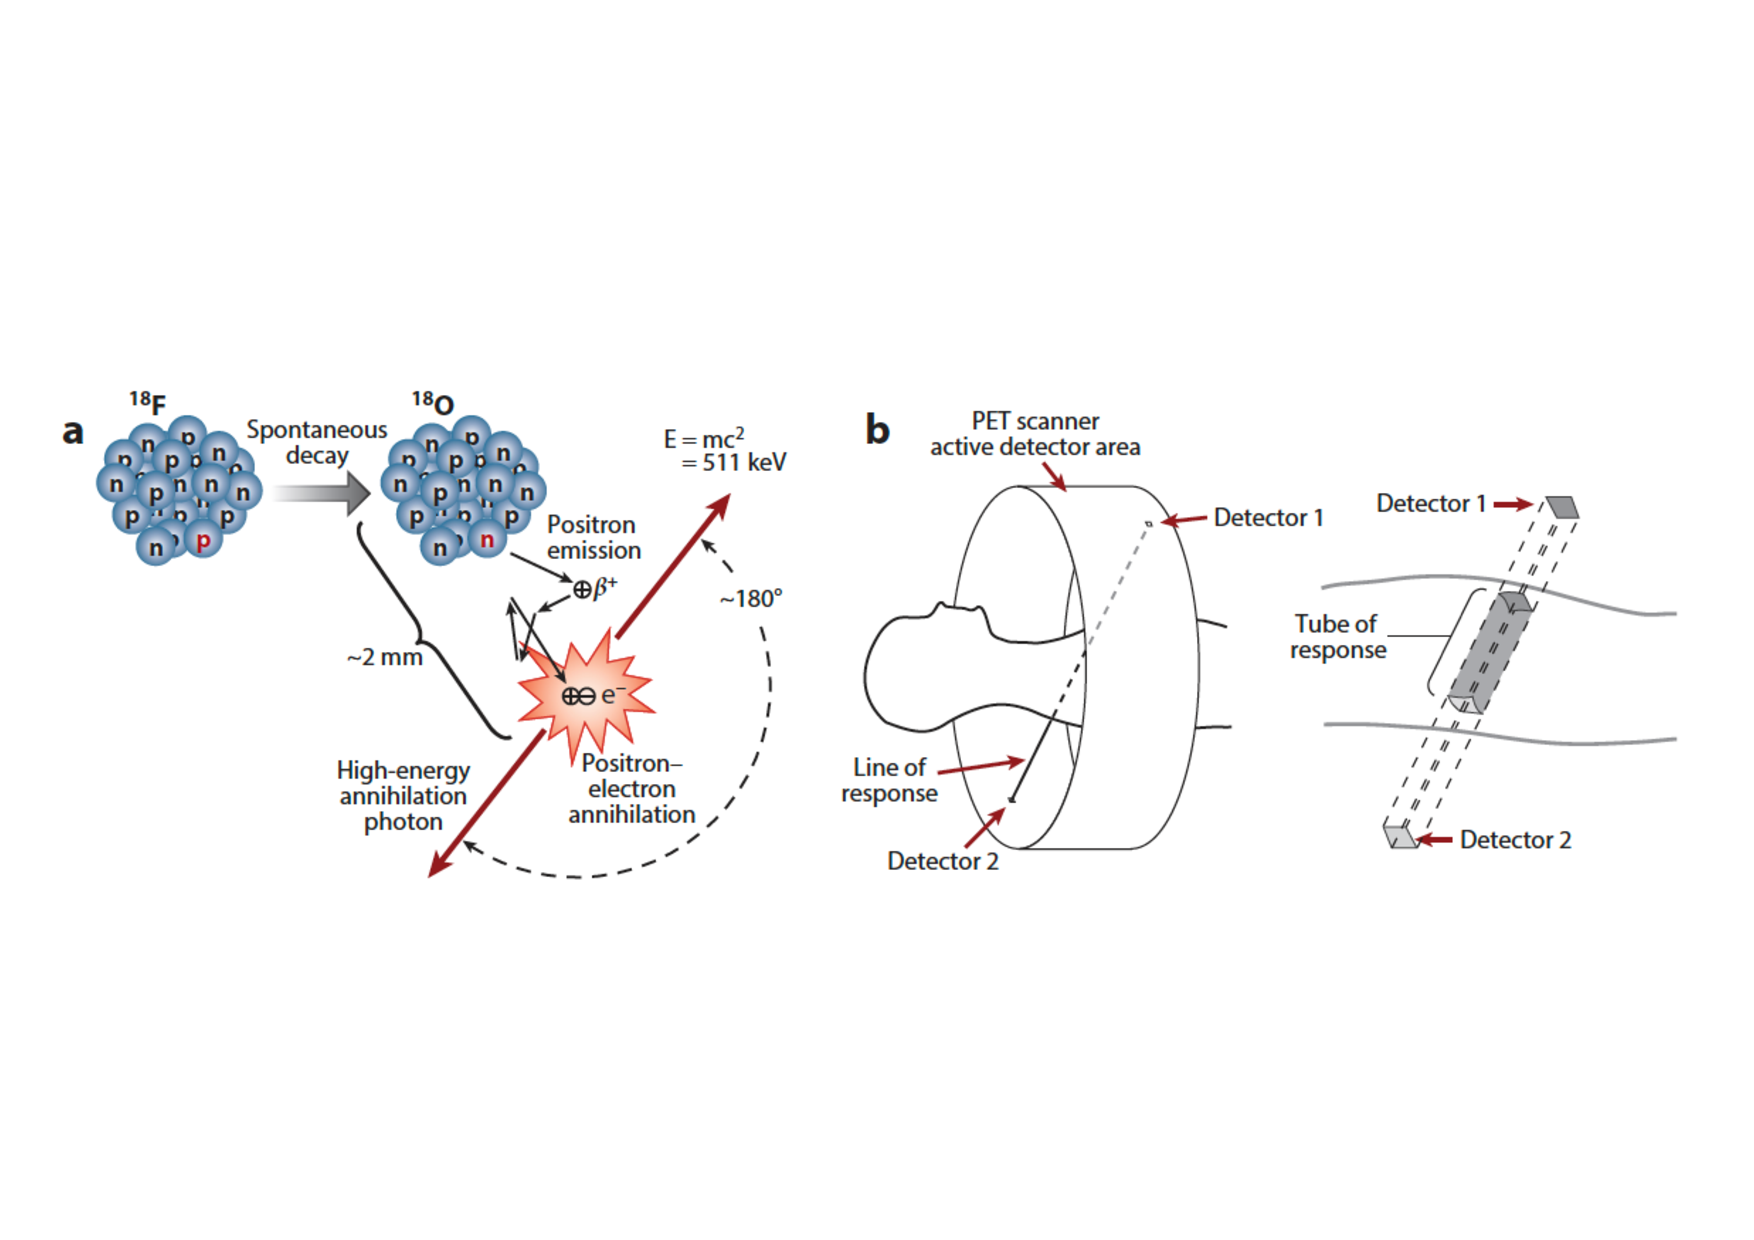
\includegraphics[width=0.8\textwidth, trim = {0 3cm 0 3cm}, clip]{03_GraphicFiles/chapter1_Introduction/NM_PET_principle.pdf}
\caption{The $\beta^{+}$ decay of $^{18}$F creates the stable isotope $^{18}$O and a positron, which travels short distance (1-2~mm) before interacting with an electron. The consequent annihilation produces two anticollinear 511~KeV photons (a). The two photons are detected by the \gls{pet} scanner in time coincidence, and the two points of interaction defines a line of response, then extended to a so-called \enquote{tube of response} which accounts for the detector's elements finite dimensions (b). In~\cite{Vaquero2015}.}
\label{chap2::fig::NM_PET_princ}
\end{figure}   
The two annihilation photons are typically detected with time coincidence windows ranging between 1 and 10~ns, depending on the specific features of the employed scanner. The spatial resolution of \gls{pet} imaging is intrinsically limited by the fundamental nature of positron annihilation, if we consider that after its creation, the positron can travel a few millimeters and follow a tortuous path through the tissue (mainly due to Coulomb scattering with electrons which can occur at large angles given the fact that the rest mass of positron is the same as the one of the electron) before reaching thermal energies and annihilating. In addition to the positron range, also the variation in the momentum of the positron leads to a limitation of the spatial resolution of \gls{pet} images. Indeed, such a variation results in an angular uncertainty in the direction of the two annihilation photons known as \enquote{noncolinearity}. Moreover, significant limitations are linked to the employed detector: the coincidence detector-pair resolution is normally specified as the \gls{fwhm} of the \gls{psf} obtained from the convolution of the two individual detector \glspl{psf}. For a detector composed of small discrete crystals, the interactions are generally assumed to take place at the center of individual crystals, and the resulting \gls{fwhm} of the coincident detector \gls{psf} is one-half the crystal size. A further factor affecting \gls{pet} imaging resolution is the parallax error, which results form the uncertainty of the \gls{doi} of the gamma rays in the crystal. Thus, unless the \gls{doi} within a crystal can be accurately determined (dedicated designs are needed), an incorrect \gls{lor} will be assigned to the interaction. A schematic representation of the parallax error is provided in \figurename~\ref{chap2::fig::PET_parallax}. The parallax error is all the more increased when the \gls{pet} ring diameter is reduced of the thickness of the crystals is increased, as the relative thickness of the detector increases. 

\begin{figure}[!htbp]
\begin{subfigure}[t]{.49\textwidth}
\centering
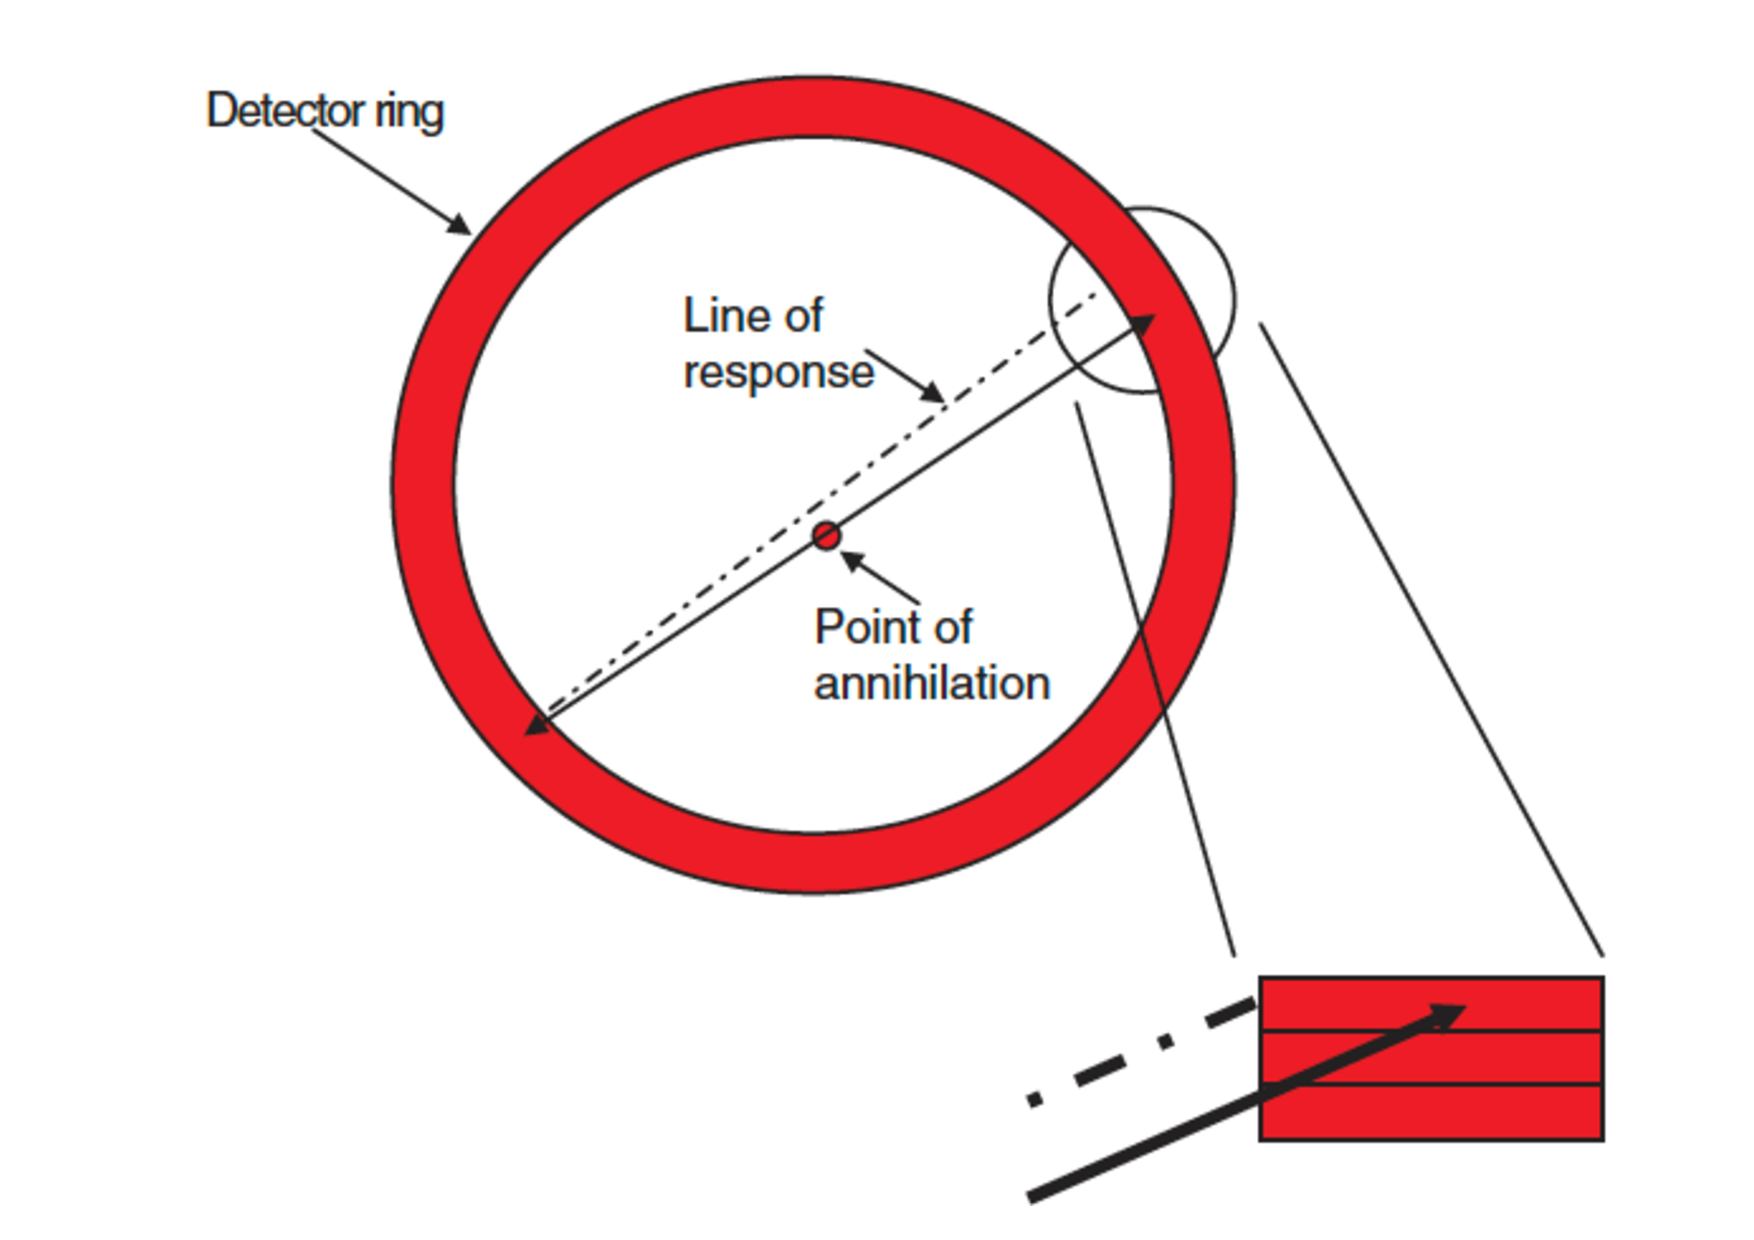
\includegraphics[width=0.7\linewidth]{03_GraphicFiles/chapter1_Introduction/PET_parallax.pdf}
\caption{Schematic view of the parallax error. The gamma ray (solid line) interacts in a crystal after penetrating one or more adjacent crystals in the detector ring. The detection electronics, if \gls{doi} information is not accessible, will incorrectly assign the \gls{lor} (dotted line) based on the front of the interaction crystal.}
\label{chap2::fig::PET_parallax}
\end{subfigure}
\begin{subfigure}[t]{.49\textwidth}
\centering
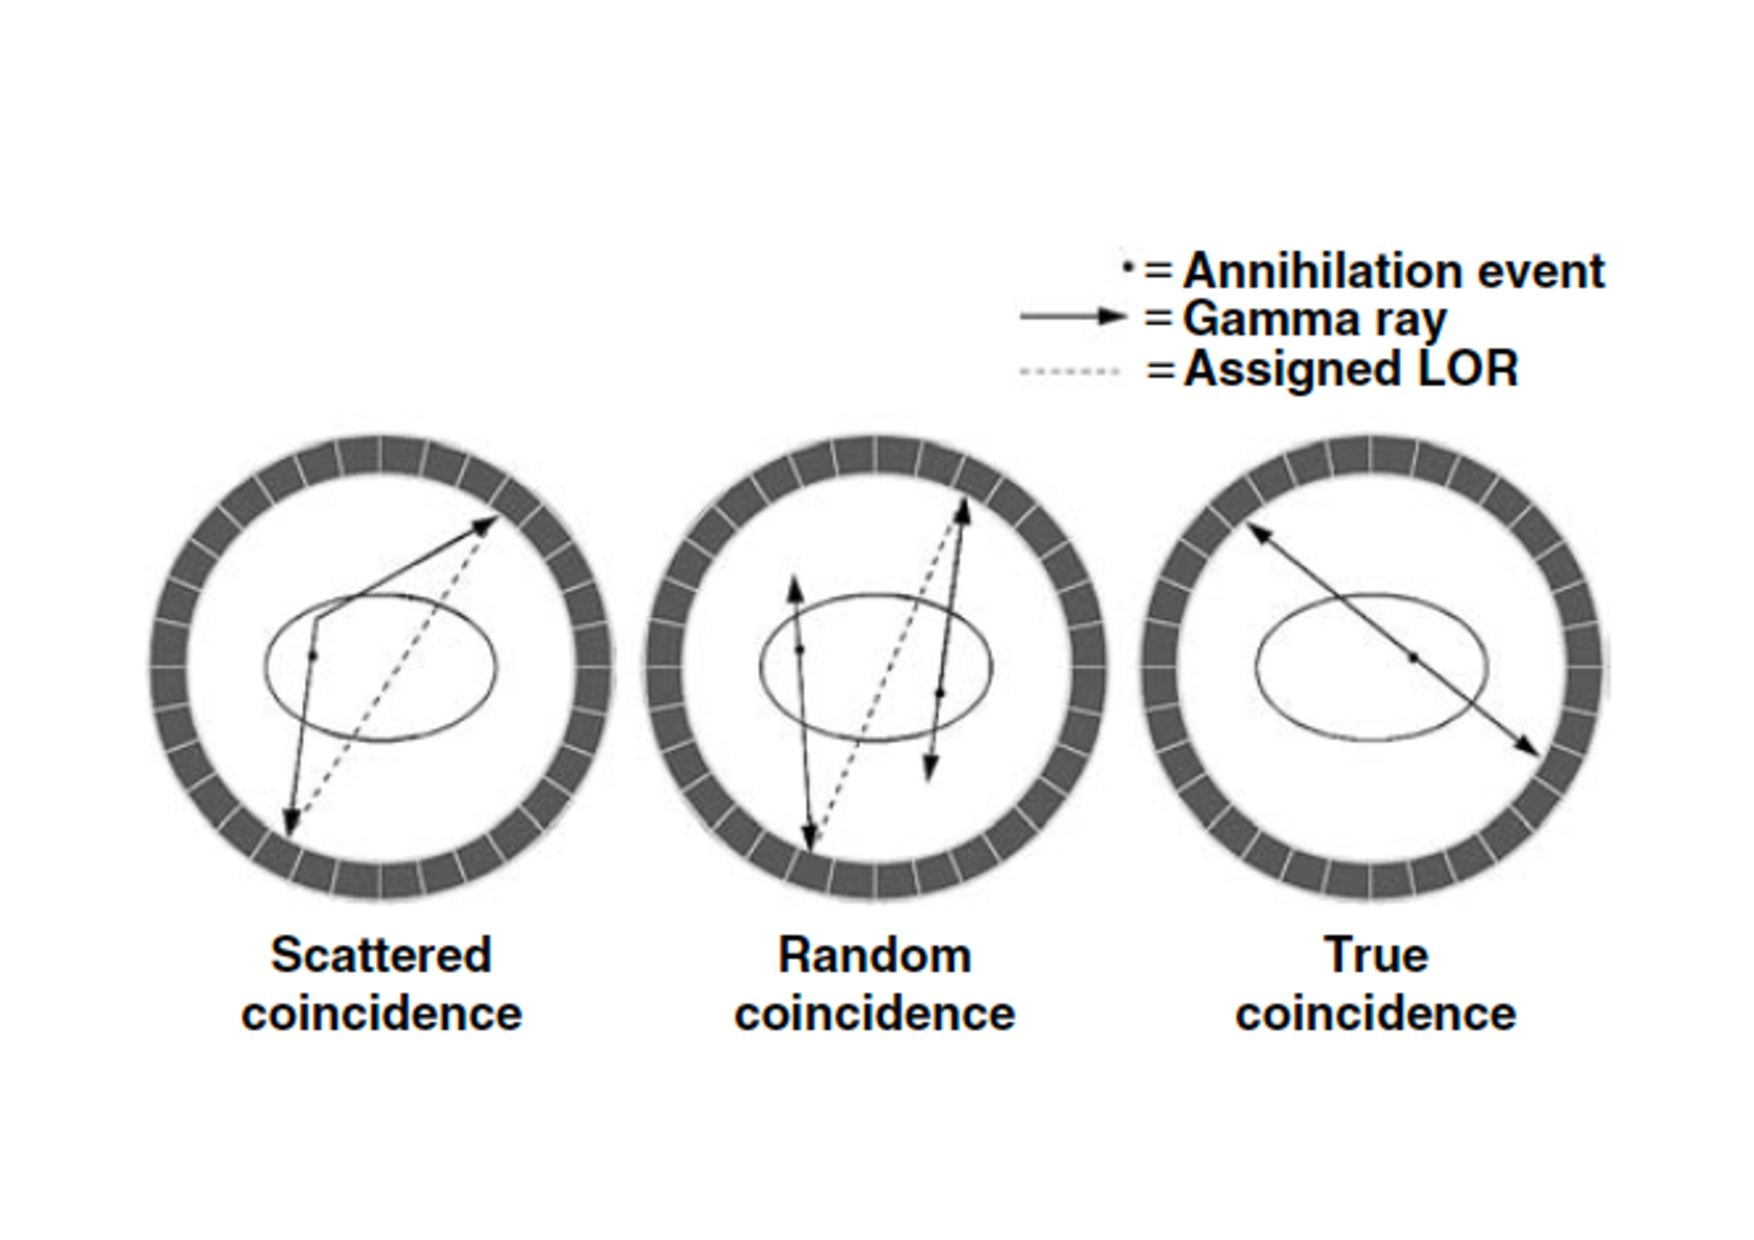
\includegraphics[width=0.98\linewidth]{03_GraphicFiles/chapter1_Introduction/PET_events.pdf}
\caption{The three types of coincidence events measured in a \gls{pet} scanner.}
\label{chap2::fig::PET_events}
\end{subfigure}
\caption{In~\cite{Lewellen2004}.}
\label{chap2::fig::PET_details}
\end{figure} 

\figurename~\ref{chap2::fig::PET_events} shows the three kinds of coincidence events that a standard \gls{pet} accepts: 
\begin{itemize}
\item true coincidences: gamma rays are detected from a single decay that have not scattered in the patient;
\item scattered events: one or both gamma rays scatter within the patient;
\item random coincidences: two separate decays result in the detection of only one gamma rays from each one and the two events are close enough in time to be in coincidence.
\end{itemize}
It is clear that increasing the number of true coincidences leads to less noise in the final image and allows one to reconstruct the collected data with high spatial resolution, and the effect of scattered coincidences can be corrected at the reconstruction stage, as well as the attenuation effect in the patient. The random coincidences are hardly treated, but their number can be reduced by decreasing the injected radiotracer activity.

The origin of the \gls{pet} imaging modality dates back to the beginning of the 50s, when a simple brain probe was used to localize brain tumors by detecting photon coincidences with 2 opposing \gls{naitl} detectors at the \gls{mgh}~\parencite{Sweet1951}. In the same year, a similar approach was published on \textit{Science} by a second reserach group~\parencite{Wrenn1951}. The development of reconstruction techniques for tomographic imaging started in the early 1960s~\parencite{Kuhl1963}, and in parallel to the first clinical trial for x-ray computed tomography the \gls{mgh} physics group developed the \gls{fbp} technique~\parencite{Chesler1971}. The first ring tomograph was built in 1973 by Robertson of \gls{bnl}, and it was composed of 32 detectors disposed in a circular array~\parencite{Robertson1972}. One year later, the PETT I (Positron Emission Transaxial Tomography) tomograph prototype was built at the Washington University by Michael E. Phelps: such a prototype was then upgraded until a human-size system, called PET III, which included extended reconstruction not limited to the transaxial plane. The system consisted of an hexagonal array with 48 \gls{naitl} detectors, and of a gantry allowing for a 60-degree rotation. With this system, the first human \gls{pet} images using the \gls{fbp} algorithm were produced~\parencite{Hoffmann1976}, marking the beginning of modern \gls{pet} development. Following the PET III development, the first commercial \gls{pet} scanner, named ECAT II (Emission Computed Axial Tomograph), was designed and put on the market; it was composed of 96 \gls{naitl} crystals, and it had a dedicated computer. The transition to commercial systems continued in the following years, and it boosted the establishment of worldwide \gls{pet} research programs. Another fundamental step in the development of the \gls{pet} technology was the discovery of \gls{bgo} scintillator. The first scanners were all based on \gls{naitl}, difficult to manufacture because of its hygroscopic nature, and with a low density, thus limited efficiency in detecting 511~keV gamma rays.  The luminescence features of \gls{bgo} were first studied by Weber at the University of California~\parencite{Weber1973}, and Nester and Huang characterized the \gls{bgo} scintillation properties in 1975~\parencite{Nestor1975}. These studies leaded to the first design and construction of a \gls{bgo}-based \gls{pet} scanner in 1978, and right after to the commercialization of the NeuroECAT, the first commercial machine to use \gls{bgo} as scintillating material. Hundreds of \gls{bgo}-based tomographs have been produced since the first introduction. 
The availability of commercial valuable \gls{pet} scanners was only one of the factor determining the spread of this imaging technique: in parallel, the development of optimized radiotracers was the second key point. Since the beginning of the \gls{pet} experience and until the second half of the 1970s, the images were obtained mainly using $^{11}$C-glucose, $^{15}$O-water and $^{13}$N-ammonia for blood flow, $^{15}$O-oxygen for oxygen utilization, and $^{18}$F fluoride for bone scans. In addition, successful molecular imaging probe was derived from the $^{14}$C-deoxyglucose. The synthesis of $^{18}$F-tagged deoxyglucose was discussed already at the beginning of the 1970s, and the Brookhaven group (Al Wolf and Joanna Fowler in particular), synthesized the first \gls{fdg}~\parencite{Ido1978}. Refined synthesis methods were developed in the following years, also thanks to the improvements of cyclotron accelerator technology, allowing for a routine basis tracer production. Nowadays, a number of companies provide small cyclotrons with various forms of automated chemistry for producing molecular imaging probes, and \gls{fdg} is still the most employed one for modern clinical \gls{pet} imaging.
During the 1980s, particular focus was dedicated to the detector side, with the development of the so-called \enquote{block detectors}: the new optical multiplexing scheme permitted to use many small scintillator pixels on a small number of \glspl{pm}, and so provided high granularity (and spatial resolution) with a limited number of read-out channels. Since 1985, the majority of \gls{pet} tomographs used some form of block detectors, which also allowed for a reduction in the scanner production cost. The introduction of this technology also increased the participation of the major imaging companies in the \gls{pet} experience: in 1986, Siemens began to distribute \gls{pet} scanners along with small cyclotrons for the production of radiotracers, and soon after also \gls{ge} entered the \gls{pet} market by purchasing the tomograph business from Scanditronix. \gls{pet} machines and imaging techniques were soon introduced in the clinical routine and approved by the main health-care systems. 
In the 1980s, research efforts have been also dedicated to the introduction of \gls{doi} capabilities in the \gls{pet} scanners to reduce parallax errors. A combination of \gls{naitl} and \gls{bgo} crystals has been used by Karp and colleagues~\parencite{Karp1987}, and the different decay time constants were used to retrieve \gls{doi} information. Various techniques have been explored in the following years to develop \gls{doi} detection capabilities, such as the introduction of multiple crystal layers in the perpendicular direction~\parencite{Liu2001} or the implementation of reflectors to create custom light-sharing patterns~\parencite{Murayama1998}. Although the research is still active on this topic, it should be considered that the effect of parallax error is small if compared with the overall resolution of the \gls{pet} scanner itself.
Further improvements came with the discovery and first grown of \gls{lso} crystals, in 1989. \gls{bgo} is very dense but has only 15\% of the light output of \gls{naitl} and relatively slow decay time (300~ns). \gls{lso} has a slightly greater density, slightly lower effective atomic number, and 5 times more light output than \gls{bgo}. Moreover, the decay time is 7.5 times faster than \gls{bgo}~\parencite{Melcher1992}. The high refinement cost initially discouraged the use of \gls{lso} for \gls{pet}, but it soon decreased thanks to the development of cost-effective techniques, so that the first \gls{lso}-\gls{pet} tomograph, microPET, was designed and fabricated in 1997~\parencite{Cherry1997}. It was designed for small animals, and commercially reproduced in 30 copies for academic programs and pharmaceutical companies. In February 1999, the first human-size \gls{lso} tomograph was delivered to the Max Planck Institute in Germany, while a combination of \gls{lso} and \gls{naitl} crystal was used for a \gls{pet}-\gls{spect} tomograph used in the Free Unviersity of Amsterdam since March 2000. 
In addition to the higher light output of \gls{lso} with respect to \gls{bgo}, leading to better spatial and energy resolution, another major advantage of this scintillator is the fast timing, which translates in lower detector dead time and in the capability to measure the time difference between the arrivals of the two annihilation photons. This \gls{tof} measurement provides positioning information which can localize the positron annihilation within a few centimeters along the line of response. A schematic view of the \gls{tof}-\gls{pet} principle is provided in \figurename~\ref{chap2::fig::NM_PET_TOF}. 

\begin{figure}[!htbp]
\centering
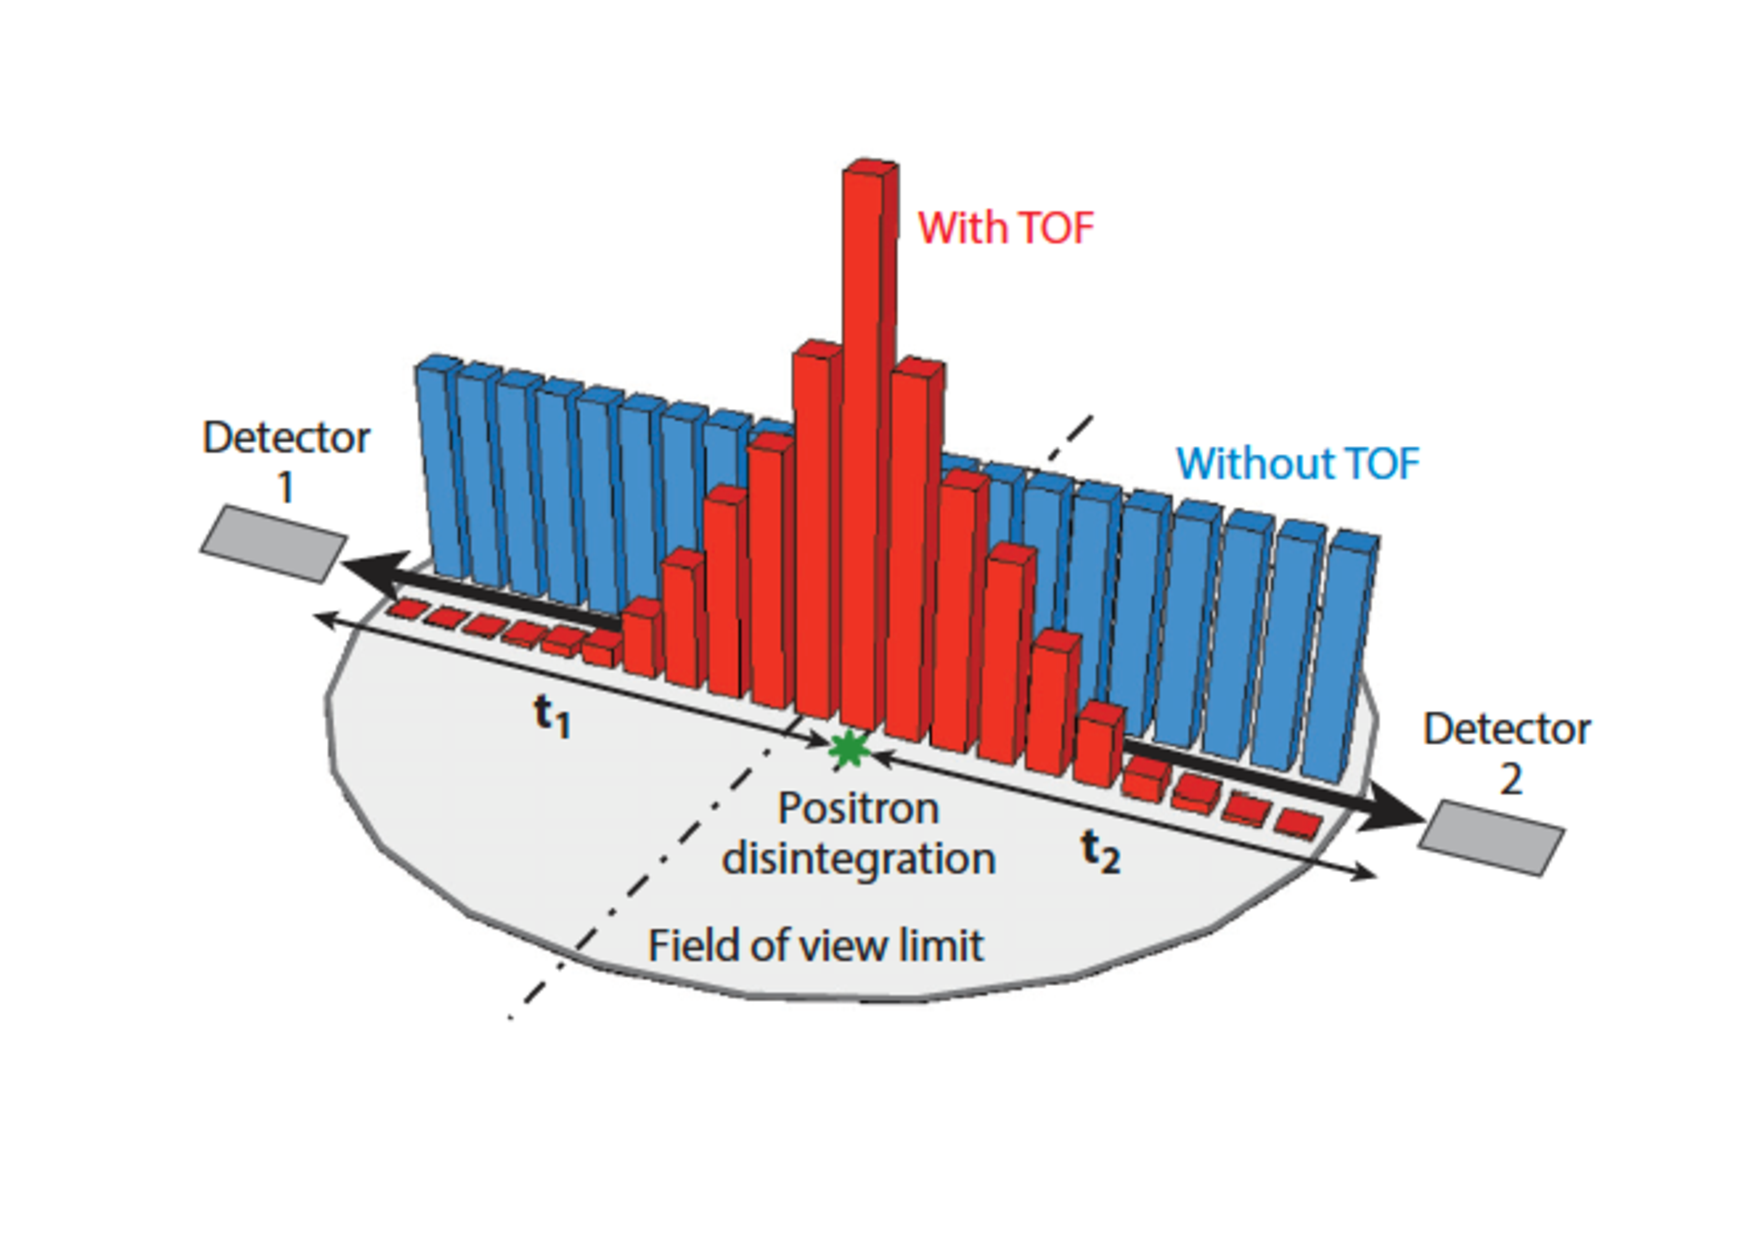
\includegraphics[width=0.8\textwidth]{03_GraphicFiles/chapter1_Introduction/PET_TOF.pdf}
\caption{Schematic view of the information provided by \gls{tof} measurement to the \gls{pet} detection. Without \gls{tof}, a flat probability is assigned to the reconstructed \gls{lor} (blue), while the measurement of the arrival time difference between the two coincident photons is translated into a distance from the \gls{lor} midpoint where the probability density function should centered (red). In~\cite{Vaquero2015}.}
\label{chap2::fig::NM_PET_TOF}
\end{figure}   

This possibility was explored already in the 1980s with fast scintillators~\parencite{Ter-Pogossian1982, Lewellen1988}, such as \gls{csf} and \gls{baf2}, which were anyway not adapted to clinical \gls{pet} application due to a low stopping power. On the other hand, the \gls{bgo} response was too slow to perform \gls{tof}. With the introduction of \gls{lso}, it was also recognized that its very good timing resolution (together with the one of the similar scintillator \gls{lyso}) could be utilized in the development of \gls{tof}-\gls{pet} systems~\parencite{Moses1999}, overcoming the limitation of the early designs of the 1980s. In 2005 Siemens presented the results from a prototype that achieved a timing resolution of 1.2~ns, and soon after the first \gls{tof}-\gls{pet} machine was launched by Philips (Philips Gemini TF)~\parencite{Karp2008}.  Based on \gls{lyso} crystal, it provided 585~ps system timing resolution. At present, all the main \gls{pet} vendors offer \gls{tof}-\gls{pet} solutions with hundreds of ps timing resolution. 
Beyond PET detector designs using conventional \glspl{pm}, the arrival of \glspl{sipm} has led to a great interest in utilizing these new photosensors to achieve improved timing resolution in \gls{tof}-\gls{pet} scanners. Philips recently introduced the Vereos system, which uses digital  \glspl{sipm} for signal readout from individual \gls{lyso} crystals; such a machine provides a system coincidence timing resolution of approximately 310 ps~\parencite{Miller2015}. In parallel \gls{ge} developed the SIGNA \gls{tof}-\gls{pet}/\gls{mri} system using a detector ring based on analog \glspl{sipm} inserted in the magnet bore, thereby
allowing simultaneous \gls{pet} and MR imaging. The reported system coincidence timing resolution of this system is 390–400~ps~\parencite{Levin2013}. Hence, while scanners with detectors using conventional \glspl{pm} are pushing closer to 400~ps timing resolution, new \gls{sipm} technology indicates that system resolution close to 300~ps is achievable with the lutetium based scintillators.
With the rapid improvements of both scintillator and photosensor technology shown by recent results, a \gls{tof} resolution below 100~ps seems achievable in the next future~\parencite{Surti2016, Lecoq2017}.
Recent studies also investigated cost-effective solutions to achieve performance comparable to present commercial systems. In particular, a whole-body \gls{pet} scanner based on plastic scintillators is being developed in Poland by the Jagiellonian University group. The J-PET is constructed with axially arranged strips of plastic scintillators, aiming to detect the annihilation photons via Compton interaction and read out on both sides by \glspl{pm}. The position of interaction in the scintillator is determined from the time difference of light signal arriving on each strip end. A \gls{tot} technique is used instead of the charge measurement of standard \gls{pet} systems in order to take advantage of the superior timing properties of plastic scintillators with respect to crystal detectors (\gls{lso} and \gls{bgo}). Preliminary studies showed that it is possible to achieve a coincidence time resolution of about 500~ps \gls{fwhm} with simple time measurements, coupled to a few millimeters spatial resolution~\parencite{Niedzwiecki2017}.

\subsection{Single Photon Emission Computed Tomography}\label{chap2::subsec::SPECT_NM}
In \gls{spect} tomographic images of the radionuclide distribution in the patient are generated from the emitted gamma photons detected as singles with collimated scintillators. Planar imaging reproduces a two-dimensional projection of the tracer distribution from a single view, while the tomographic image is obtained by the reconstruction of several slices collected from multiple camera positions. Both techniques are used in clinics: planar imaging is less demanding and only requires a single camera head, while multiple camera heads mounted on a rotating gantry are generally used for tomographic imaging, and image reconstruction is required.

Although many innovations have been made since the introduction of the first gamma camera in 1958 by Hal Anger~\parencite{Anger1958}, today's clinical detectors share many of the essential features of Anger's early designs, and are often called Anger cameras. A standard \gls{spect} gamma camera is composed of an aperture or collimator which mechanically selects photons traveling in specific directions, depending on the collimator configuration. The photons approaching the camera from directions different than those specified by the collimation system are passively absorbed. The gamma photons with the selected direction then encounter a scintillation detectors coupled to photosensors. The related electronics and data acquisition system are generally optimized to impose energy threshold in order to reject undesired photons, such the ones which underwent scattering in the collimator section. A schematic view of the main component of the \gls{spect} camera is given in \figurename~\ref{chap2::fig::SPECT_components}, while a simplified view of the collimation principle is sketched in \figurename~\ref{chap2::fig::SPECT_collimator}.   

 \begin{figure}[!htbp]
\begin{subfigure}[t]{.49\textwidth}
\centering
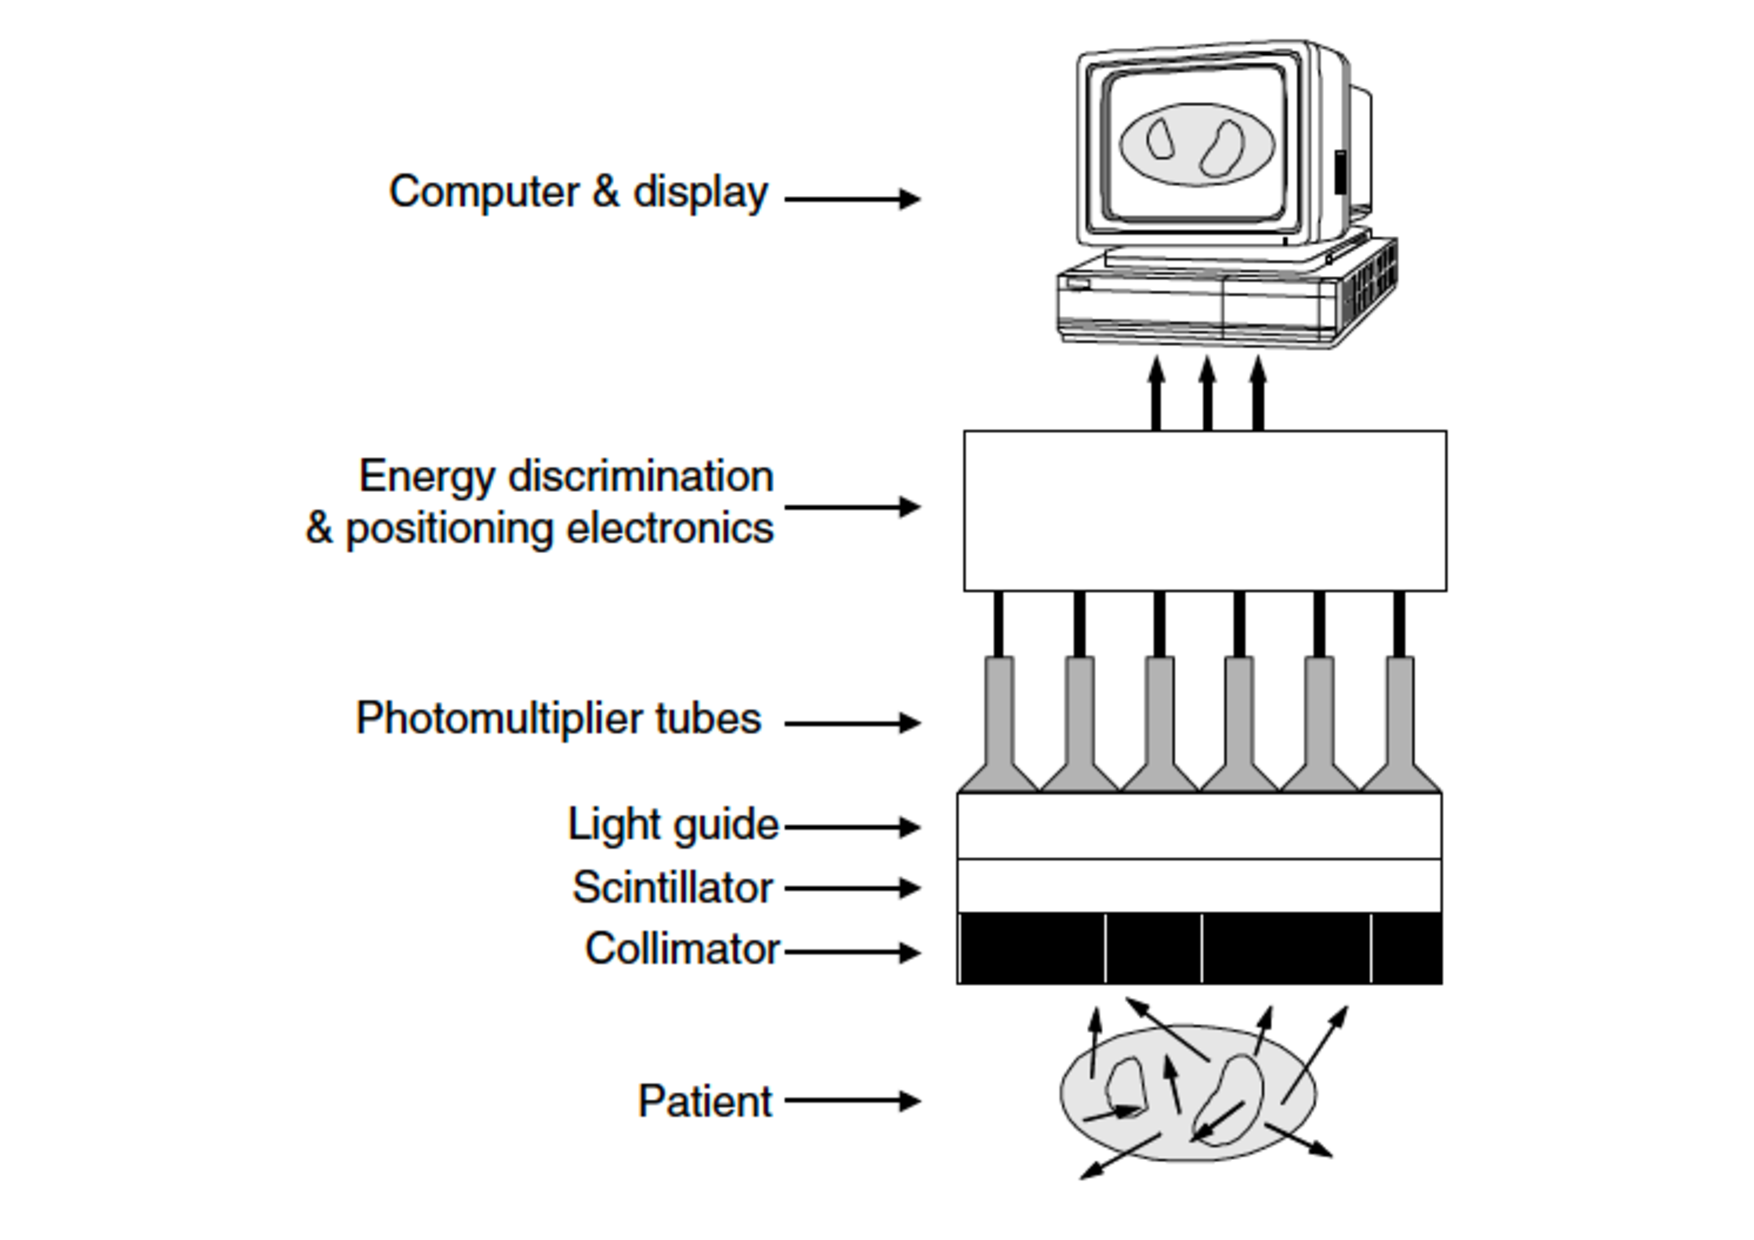
\includegraphics[width=0.98\linewidth]{03_GraphicFiles/chapter1_Introduction/SPECT_components.pdf}
\caption{Schematic view of the main components of a \gls{spect} gamma camera.}
\label{chap2::fig::SPECT_components}
\end{subfigure}
\begin{subfigure}[t]{.49\textwidth}
\centering
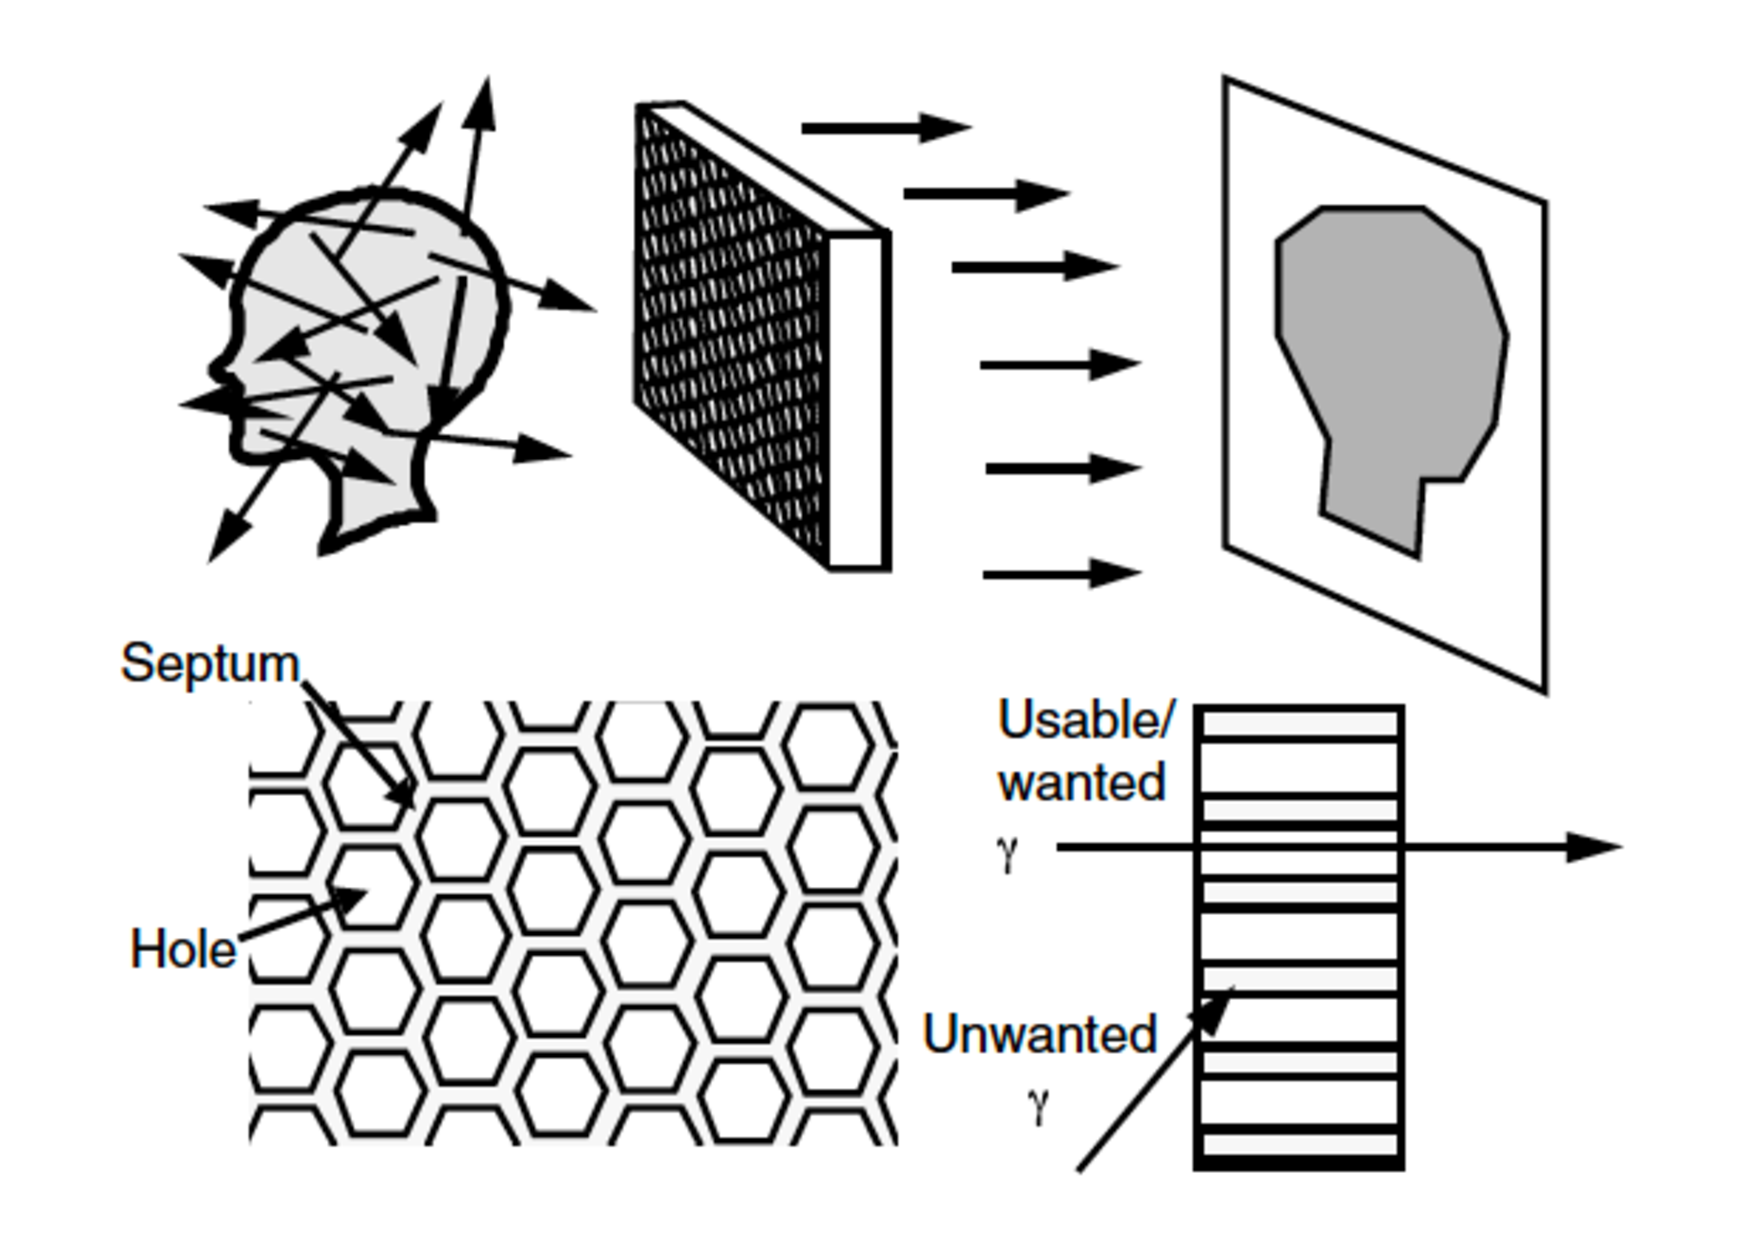
\includegraphics[width=0.98\linewidth]{03_GraphicFiles/chapter1_Introduction/SPECT_collimator.pdf}
\caption{Schematic representation of the collimation principle of \gls{spect} gamma cameras.}
\label{chap2::fig::SPECT_collimator}
\end{subfigure}
\caption{In~\cite{Zeng2004}.}
\label{chap2::fig::SPECT_details}
\end{figure} 

The most simple photon passive selection device is the pinhole aperture, but acceptable spatial resolution can be only obtained at the expense of the system sensitivity. Improved, but always limited overall sensitivity is provided by the introduction of collimators, composed of array of holes separated by septa.  Collimator septa are composed of highly absorbing material with high atomic number and high density. Alloys of lead, tungsten and gold are the most common materials used for this purpose. 
Various hole shapes (circular, square, triangular or hexagonal) are used in common collimators, but the hexagonal shape is the most diffused because it provides the best efficiency. In addition to parallel hole patterns, also converging and diverging collimators have been developed. Converging collimators magnify an image on a camera face and thus can yield finer resolution and/or higher sensitivity images than those resulting from used of parallel-hole collimators. Converging solutions are adapted to small-size objects with respect to the camera \gls{fov}, while the image of large object would result truncated (if part of the object is outside the \gls{fov} of the camera) or distorted (because the magnification is dependent on the distance from the collimator). 
The most spread parallel-hole collimators find routine use in clinics in four configurations: \gls{lehr}, \gls{legp}, \gls{megp}, and \gls{hegp}. Each designation is adapted to a defined gamma energy range, and thus to certain radioisotopes, and is also an indication of the trade-off between resolution and sensitivity which are affected by the septal material, the hole size and length, and the septal thickness. Collimator sensitivity is maximized by the thinnest possible septa, but thin septa can lead to septal penetration which is extremely detrimental to diagnostic performance. The aforementioned trade-off is then a crucial parameter to be considered when designing a \gls{spect} camera, and, together with the employed scintillator and photosensor features, completely determine the overall system performance~\parencite{Gunter2004}.

The origins of \gls{spect} imaging can be identified with the invention of the Anger scintillation camera in the late 1950s~\parencite{Anger1958, Anger1964}; previously, scans were performed by manually positioning a Geiger counter above the organ of interest, but with the Anger camera the entire organ could be scanned at one time. During the 1960s, both longitudinal and transaxial emission tomography were deeply studied. Crandall and Cassen developed a longitudinal tomographic scanner which used a highly focusing collimator placed on a large crystal-matrix detector~\parencite{Crandall1966}, and in 1969, Anger invented a sophisticated longitudinal tomograph that used a scanning scintillation camera~\parencite{Anger1969}. Transaxial tomographs were developed by Kuhl and colleagues between 1963 and 1976, and the final prototype used discrete scintillator arrays~\parencite{Kuhl1976}. Discrete scintillation detectors have been also used for other scanners in the late 1970s, but the first investigators to explore the possible implementation of an Anger camera for transaxial tomography were Paul Harper and colleagues at the University of Chicago. In the early stages, a rotatable chair was placed in fornt of a single head fixed Anger camera~\parencite{Muehllehner1971}. In 1976, Jaszczak and Keyes, independently developed a \gls{spect} system that used an Anger camera mounted on a rotating gantry~\parencite{Jaszczak1977, Keyes1977}. In the following years, the first whole-body \gls{spect} system was developed and clinically evaluated in 1978 at the Baylor College of Medicine~\parencite{Jaszczak1979}. During the late 1970s and the 1980s, both rotating-camera \gls{spect} systems and stationary detector configurations were proposed and developed in Europe and US~\parencite{Larsson1980, Rogers1988}, and the bases for modern machines were established. 
The modern cameras, as mentioned, rely on the described designs and have been adapted.in the past years, to new tracers provided by the pharmaceutical industry. \gls{spect} takes advantage of many years of experience and is now a well-established imaging modality in nuclear medicine. Thanks to its cost-effectiveness, such an imaging technique is widely employed in the clinical routine, and all the major medical imaging companies offer a \gls{spect} system, generally in dual-head configuration with rotating gantry.
At present, virtually all single-photon imaging\myMarginnote{Compton cameras for SPECT} in nuclear medicine relies on Anger-type cameras, relatively simple and cost-effective, but limited in sensitivity and energy acceptance given the presence of a mechanical photon selection system. Already in 1974 this limitation was addressed by Todd and Nightingale which proposed the application of Compton imaging methods to nuclear medicine~\parencite{Todd1974}. The Compton detection principle is described in section~\ref{chap2::subsubsec::PGI_elecColl}. To be noticed that for the application in nuclear medicine, the detector design is less constraint then in ion range monitoring, given the \textit{a priori} knowledge of the incident photon energy.
Starting from 1981, Singh and colleagues published a number of seminal papers that described analytical and experimental results for Compton camera composed of a pixelated germanium first detector and a standard Anger camera as second detector~\parencite{Singh1981, Singh1983, Singh1983b}. The investigation of such an imaging modality for the application in single photon detection for nuclear medicine continued in the following years. More recently, a prostate probe hs been proposed and built by Llosa and colleagues, based on Compton imaging exploited by a composition of silicon sensors (4$\times$1~cm with 256 pads) and \gls{naitl} scintillators (16$\times$16$\times$1.27~cm$^3$). The prototype has been tested with $^{57}$Co and $^{133}$Ba sources~\parencite{Llosa2006}, and a spatial resolution of 5~mm \gls{fwhm} for the imaging of a point-like$^{133}$Ba source has been reported~\parencite{Llosa2008}. After a first prototype essentially developed for hihg-energy astrophysics observations~\parencite{Takeda2007}, a Japanese group optimized a Compton device based on silicon and \gls{cdte} detectors fro high spatial resolution, and proposed its application in nuclear medicine~\parencite{Takeda2009}. The prototype, then optimized for biomedical application and described in~\cite{Takeda2012}, consists of a 2.56$\times$2.56-cm \gls{dssd}vand four layers of pixelated \gls{cdte} detectors.The thickness of each detector is 0.5~mm. The device has been tested with rats and the resulting spatial resolution in the three dimensions was 8$\times$8$\times$10~mm~\parencite{Suzuki2013}, similar to the one of clinical \gls{spect} systems, but poorer with respect to \gls{pet} machines~\parencite{Madsen2007}. However, improvements and spatial resolution similar or superior with respect to standard \gls{pet} are expected. The same conclusions have been presented by the authors concerning the device efficiency, which was very low during the animal experiments, but orders of magnitude higher in astrophysics observations with previous prototypes. Notwithstanding the highlighted limitations, the capability of three dimensional image reconstruction in clinical condition has been verified.
\gls{dssd} layers and \gls{naitl} crystals are also the basic components of a double-scattering Compton camera developed by a Korean research group. First studied in \gls{mc} simulations~\parencite{Seo2007}, the system is composed of two identical 50$\times$50$\times$1.5~mm$^3$ silicon layers and a \gls{naitl} scintillator crystal, 3 inches diameter $\times$ 3 inches height. Preliminary tests with a point-like $^{22}$Na source showed a spatial resolution of 9.0 and 4.8~mm for 511~kev and 1275~keV photons, respectively~\parencite{Seo2010}. The device has also been tested with gamma sources placed inside anthropomorphic phantoms: in particular, $^{22}$Na and $^{137}$Cs have been used, and a spatial resolution below 15~mm has been showed in both cases~\parencite{Seo2011}. The application of such a prototype to ion beam range verification has also be envisaged. 
The performance of a Compton camera based on pixelated germanium detectors have been evaluated and are presented in~\parencite{Alnaaimi2011}. Although the camera demonstrated the ability to image distributed sources, some limitations in acquisition and image processing time have been highlighted. 
The ETCC camera~\parencite{Kabuki2007} presented in section~\ref{chap2::subsubsec::PGI_elecColl} has been also tested for nuclear medicine applications with the imaging of nucleat medicine common reagents~\parencite{Kabuki2009}. The camera has also been used for phantom and small animal tests: in particular, the brain of mice has been imaged with \gls{fdg} tracer, and the comparison with conventional \gls{pet} data showed a good agreement. In addition, the camera also succeeded in th imaging of multiple tracers (\gls{fdg} and $^{131}$I isotope)~\parencite{Kabuki2010}.
The field is still today actively explored: in particular, the availability of new high-energy tracers could provide advantages in terms of dose and spatial accuracy, but high-energy photons are hardly collimated with mechanical passive system. The electronic collimation exploited by Compton cameras can be the solution for high-sensitivity and high-resolution \gls{spect} examinations. 
More details can be found in in chapter~\ref{chap::5} of this thesis, where the described topic has been addressed with simulation studies. The presented results have been recently published in~\parencite{Fontana2017_PMB} and~\parencite{Fontana2017_APPB}. 

\subsection{Theranostics}\label{chap2::subsec::Theranostics}

The theranostics approach in nuclear medicine couples diagnostic imaging and cancer therapy using the same molecule or at least very similar drugs, given in different dosages. For example, the combination of \gls{iod131} (gamma emitter) and \gls{lut177} (beta emitter), is used for both imaging and therapy. Furthermore, different isotopes of the same elements (for example \gls{iod123}, \gls{iod131} and the newer terbium isotopes - Tb) can also be used for theranostics given the multiple associated emission (beta and gamma, gamma rays at different energies, alpha and gamma)~\parencite{Gerard2002, Alzahrani2012, Muller2012}. During the treatment, theranostics can be applied in monitoring the therapy course and estimating the potential response and eventual toxicity. The safety of high cumulative doses of radioactive agents after multiple repeated cycles is, however, a cause of concern. Anyway, remarkable improvements have been obtained in targeted therapies, which have proven to be effective with favorable safety profiles~\parencite{Baum2012, Kwekkeboom2008, Strosberg2017}. The diagnostic part of theranostics can be performed with both \gls{pet} and \gls{spect} machines, depending on the employed radioisotope emissions. Most therapeutic radiopharmaceuticals are labeled with $\beta^{-}$-emitting isotopes, having a tissue penetration of only few millimeters and so adapted to spare the healthy tissues surrounding the tumor. The first theranostic radiopharmaceutical in nuclear medicine history was radioiodine, used for therapy and imaging in thyroid diseases~\parencite{Hertz2016}. iodine is taken up by the thyroid galnd for the production of hormones, vital for the development of the brain, normal growth and metabolic balance. In 19367, Hertz developed the idea of administrating radioactive iodine in patients with thyroid diseases, and few years of preclinical studies at the \gls{mit} (where the first cyclotron for medical use had been built) followed this first proposal. In 1941, the first patient was treated with radioiodine~\parencite{Hertz1942}. \gls{iod131} is to the date the gold standard for certain therapeutical indications, given its low cost and the advantageous combination of $\beta^{-}$ and gamma emission. The electron radiation targets the thyroid from the inside, while the organ can be visualized using a gamma camera. 

Since its first proposal, the use of theranostic agents has been consistently increasing: the combination of targeted cancer imaging and therapy is a considerable contribution to personalized medicine and may play an important role in the future with the implementation of new chemical agents and the continuous improvement of imaging systems~\parencite{Yordanova2017}. For the peculiar context of this thesis it is worth to notice that, as for diagnosis \gls{spect}, high-energy gamma emitters can be applied in theranostics, and Compton camera can be implemented for the imaging task. This point is further discussed in chapter~\ref{chap::5}. 

\section{Image reconstruction}\label{chap2::sec::Image_reconstruction}

Regardless of their specific application, imaging-related data sets have to be reconstructed in order to obtain the desired image. Nuclear medicine and \gls{pg} detection devices share the basic reconstruction approaches, and peculiar algorithms have been developed for each application. In particular, image reconstruction approaches can be classified in analytic and iterative methods. Analytic algorithms are generally founded on back-projections, with further steps of filtering and regularization that could be added to the reconstruction process in order to provide enhanced accuracy. In the particular case of nuclear medicine, tomographic reconstruction algorithms are used in \gls{pet} and \gls{spect} to obtain three-dimensional information. Improvements over the analytic approach are usually provided by the iterative one, able to profit from more realistic model of the system as well as to account for image noise components. This better performance comes at the expense to algorithm complexity and calculation time. Iterative methods start from a model of the final image, generally corresponding to a regular geometric surface/volume divided into a defined number of equivalent pixels/voxels. The system is modeled in order to connect the image to the collected data: each element of the model represents the probability that the emission of a given collected gamma ray is related to a specific pixel/voxel. In order to model the data, since the gamma detection is Poisson distributed, a Poisson approach is implemented to describe in statistical terms the relationship between the value of the measurements and the expected value of the measurements. Modified Poisson statistical models and Gaussian models are also used, given the fact that after physical data corrections (attenuation, scatter, randoms, etc.) the data sets could diverge from a Poisson distribution. Once this first definition steps are accomplished, a principle governing the process iterations must be defined to converge to the \enquote{best image}. The Maximum Likelihood approach is probably the most intensively studied and used, at present, in medical imaging, but alternative methods are available. Finally, an algorithm must be created to find the best image according to the defined models and iteration principle. The Expectation Maximization algorithm is the most diffused one, and can be adopted in several variations according to the specific application and objectives. 

In the following sections, the two algorithms used during this thesis work to reconstruct the \gls{clarys} Compton camera data are described in more details.

\subsection{Line-cone analytic reconstruction}\label{chap2::subsec::LineConeRec} 

The analytic reconstruction of Compton camera collected data gives, for each event, a cone surface on which the gamma emission point must lie. In the particular case of the Compton camera application in ion range monitoring, the \textit{a priori} knowledge of the beam direction can be included in the reconstruction point: the intersection of each reconstructed cone with the beam line results in two single points per event. The mono-dimensional distribution of the gamma emission points can be then reconstructed in the beam direction. This is the basic principle of the line-cone analytic reconstruction, which is used to reconstruct the Compton camera data; reconstructed profiles obtained with simulated data are shown in chapter~\ref{chap::4}.
Alternative analytic reconstruction methods are proposed in other studies~\parencite{Cree1994, Basko1998, Parra1999, Hirasawa2003, Maxim2009}. 

\subsection{Iterative reconstruction of Compton camera data}\label{chap2::subsec::IterRec} 

The iterative reconstruction approach allows to account for image background components and include the detector energy and spatial resolutions, and results in a three-dimensional image. Several algorithms have been proposed for the reconstruction of Compton events, based on the main points listed above~\parencite{Schone2010, Zoglauer2011, Gillam2011, Andreyev2011, Mackin2012, Huang2018, Taya2017, Schone2017}. The data related to the \gls{clarys} Compton camera have been reconstructed with a \gls{lm-mlem} algorithm, a version of the \gls{mlem} method based on the list of detected events. It has been developed by the \gls{creatis} group, which is actively working in this field in collaboration with the \gls{ipnl}~\parencite{Maxim2009, Lojacono2013, Hilaire2014}.
The first step is to define the volume which includes the origin of the prompt gamma ray detected. This volume is divided into equal voxels and the emission intensity is assumed homogeneous for each voxel $j$, with a Poisson distribution of parameter $\lambda_j$ (a vector of the emissions intensities of all the voxels). The algorithm is based on a system matrix $T$ composed of the coefficients $t_{ij}$ which represent the probability that a photon produced in the voxel $j$ is detected in coincidence by the Compton camera as an event $i$. The probability for a gamma detected in coincidence to be emitted from the voxel $j$ is denoted as $s_j$.
The \gls{lm-mlem}valgorithm starts with an initial value $\lambda^{(0)}_j$, which can be the simple back-projection reconstruction.
The iterations rely on the recurrence relation in equation~\ref{chap2::eq::equation_lambda_compton_NM}.

\begin{equation}
\lambda_j^{(l+1)} =  \frac{\lambda_j^{(l)} }{s_j} \sum\limits_{i=1}^{N_{\gamma}} t_{ij} \frac{1}{P_i^{(l)}},\quad \mathrm{with}\quad  P_i^{(l)}=\sum\limits_{k=1}^{N_{v}} t_{ij}\lambda_k^{(l)},
 \label{chap2::eq::equation_lambda_compton_NM}
\end{equation}
where $N_{\gamma}$ is the number of detected events and $N_v$ is the number of voxels in the image.

For each photon detected, the coefficients in column $i$ are calculated by taking into account the uncertainties on the angle between the source and the involved scatterer plane and the angle between the scatterer plane and the absorber involved module.
The matrix elements $t_{ij}$ are calculated as in equation~\ref{chap2::eq::equation_tij_compton_NM}.
\begin{equation}
 t_{ij} = K(\beta_i,E_{tot})\frac{|\mathrm{cos}(\theta_{{V_2V_1}}) |}{V_2V_1^2} \int\limits_{M\in v_j} \frac{|\mathrm{cos}(\theta_{V_1M})|}{V_1M^2} h_i(M)dv,
 \label{chap2::eq::equation_tij_compton_NM}
\end{equation}
where $\beta_i$ is the Compton scattering angle, $V_1$ the interaction position in the scatterer, $V_2$ the interaction position in the absorber, $h_i$ the spatial kernel which models the uncertainties on the Compton angle for each voxel $M$, $K(\beta_i,E_{tot})$ the differential cross section and $v_j$ the reconstructed volume.

In order to simplify and speed up the calculation of the $t_{ij}$ matrix, the voxels located far from the reconstructed cone are set to zero. The distance between the cone and the voxel is calculated by taking the voxel center as reference point. 
For each iteration, the matrix $T$ is stored and the reconstructed image can be produced.

The algorithm has been used to reconstruct the simulated data produced to test the \gls{clarys} Compton prototype for particle therapy monitoring and nuclear medicine, and the results are presented in chapter~\ref{chap::4} and chapter~\ref{chap::5}, respectively. 



\clearpage
%\printbibliography[heading=subbibintoc]
